\documentclass[acmsmall,nonacm]{acmart}
\settopmatter{printfolios=true,printccs=true,printacmref=false}

\usepackage[capitalise,noabbrev]{cleveref}
\usepackage[inline]{enumitem}
\usepackage{extarrows}
\usepackage{apxproof}
\usepackage{longtable}
\usepackage{adjustbox}
\usepackage{url}
\usepackage{multicol}
\usepackage{stmaryrd}
\usepackage{proof}
\usepackage{bbold}
\usepackage{subcaption}
\usepackage[utf8]{inputenc}
\usepackage{newunicodechar}
\usepackage{underoverlap}

\let\Bbbk\relax
\usepackage{amssymb}
\usepackage{newtxmath}

\usepackage{agda}
\AgdaNoSpaceAroundCode
\renewcommand{\AgdaCodeStyle}{\footnotesize}

\usepackage{tikz}
\usetikzlibrary{decorations.markings}
\usetikzlibrary{quotes,fit,positioning}
\usetikzlibrary{knots}
\tikzstyle{func}=[rectangle,draw,fill=black!20,minimum size=1.9em,text width=2.4em, text centered]
\usetikzlibrary{braids}
\tikzset{>=latex}
\usepackage{tikzit}
../paper/tikzit.sty
\usepackage{quiver}

\usepackage{macros}
\usepackage{hott}
\usepackage{syntax}

% \usepackage[
%   all=normal,
%   paragraphs,
%   floats,
%   wordspacing,
%   charwidths,
%   mathdisplays,
%   indent,
% ]{savetrees}

%% Some recommended packages.
%% \usepackage{booktabs}   %% For formal tables:
                        %% http://ctan.org/pkg/booktabs
%% \usepackage{subcaption} %% For complex figures with subfigures/subcaptions
                        %% http://ctan.org/pkg/subcaption
%% \usepackage{verbatim}
%% \usepackage{amsmath,amsbsy}
%% \usepackage{alltt}
%% \usepackage{fdsymbol}
%% \usepackage{amsthm,proof}
%% \usepackage{bbold,stmaryrd,bbm}
%% \usepackage{ucs}
%% \usepackage{wrapfig}
%% \usepackage[utf8x]{inputenc}
%% \usepackage{microtype}
%% \usepackage{agda}
%% \usepackage{mathtools}
%% \usepackage{amsthm,amsmath}
\usepackage[nocenter]{qtree}
%% \usepackage{listings}

\newtheorem{theorem}{Theorem}
\newtheorem{corollary}[theorem]{Corollary}
\newtheorem{lemma}[theorem]{Lemma}
\newtheorem{definition}[theorem]{Definition}
\newtheorem*{remark}{Remark}
\newtheoremrep{proprep}[theorem]{Proposition}

\newtheoremrep{theorem}{Theorem}[section]
\newtheoremrep{corollary}[theorem]{Corollary}
\newtheoremrep{proposition}[theorem]{Proposition}
\newtheoremrep{lemma}[theorem]{Lemma}
\newtheoremrep{definition}[theorem]{Definition}

\newunicodechar{⊸}{$\multimap$}
\newunicodechar{𝕍}{$\mathbb{V}$}
\newunicodechar{𝕃}{$\mathbb{L}$}
\newunicodechar{𝕄}{$\mathbb{M}$}
\newunicodechar{ℝ}{$\mathbb{R}$}
\newunicodechar{𝕌}{$\mathbb{U}$}
\newunicodechar{𝔹}{$\mathbb{B}$}
\newunicodechar{𝕐}{$\mathbb{Y}$}
\newunicodechar{𝔼}{$\mathbb{E}$}
\newunicodechar{𝔽}{$\mathbb{F}$}
\newunicodechar{𝕋}{$\mathbb{T}$}
\newunicodechar{𝕚}{$\mathbb{i}$}
\newunicodechar{𝟘}{$\mathbb{0}$}
\newunicodechar{𝟙}{$\mathbb{1}$}
\newunicodechar{𝟚}{$\mathbb{2}$}
\newunicodechar{𝟛}{$\mathbb{3}$}
\newunicodechar{𝟠}{$\mathbb{8}$}
\newunicodechar{⟷}{$\leftrightarrow$}
\newunicodechar{₀}{$_{0}$}
\newunicodechar{₁}{$_{1}$}
\newunicodechar{₂}{$_{2}$}
\newunicodechar{₃}{$_{3}$}
\newunicodechar{₄}{$_{4}$}
\newunicodechar{■}{$\blacksquare$}
\newunicodechar{⊡}{$\boxdot$}
\newunicodechar{⋆}{$\star$}
\newunicodechar{◎}{$\circledcirc$}
\newunicodechar{⊗}{$\otimes$}
\newunicodechar{⊕}{$\oplus$}
\newunicodechar{₊}{$_{+}$}
\newunicodechar{↔}{$\leftrightarrow$}
\newunicodechar{⇔}{$\Leftrightarrow$}
\newunicodechar{∀}{$\forall$}
\newunicodechar{ϕ}{$\phi$}
% agda --latex ../Examples/ExamplesL.lagda
\input{\detokenize{ExamplesL.tex}}

%%
%% \BibTeX command to typeset BibTeX logo in the docs
\AtBeginDocument{%
  \providecommand\BibTeX{{%
    \normalfont B\kern-0.5em{\scshape i\kern-0.25em b}\kern-0.8em\TeX}}}



%% Journal information
%% Supplied to authors by publisher for camera-ready submission;
%% use defaults for review submission.
\acmJournal{PACMPL}
\acmVolume{1}
\acmNumber{POPL} % CONF = POPL or ICFP or OOPSLA
\acmArticle{1}
\acmYear{2022}
\acmMonth{1}
\acmDOI{} % \acmDOI{10.1145/nnnnnnn.nnnnnnn}
\startPage{1}

%% Copyright information
%% Supplied to authors (based on authors' rights management selection;
%% see authors.acm.org) by publisher for camera-ready submission;
%% use 'none' for review submission.
%\setcopyright{none}
%\setcopyright{acmcopyright}
%\setcopyright{acmlicensed}
\setcopyright{rightsretained}
%\copyrightyear{2018}           %% If different from \acmYear

%% Bibliography style
\bibliographystyle{ACM-Reference-Format}
%% Citation style
%% Note: author/year citations are required for papers published as an
%% issue of PACMPL.
\citestyle{acmauthoryear}   %% For author/year citations

%%
%% end of the preamble, start of the body of the document source.
\begin{document}

%%
%% The "title" command has an optional parameter,
%% allowing the author to define a "short title" to be used in page headers.

\title{Symmetries in Reversible Programming}
\subtitle{From Symmetric Rig Groupoids to Reversible Programming Languages}

% Reversible Programming with Univalent Finite Types
% Curry-Lambek Correspondence between Reversible Circuits and Symmetric Rig Groupoids
% Reversible Curry-(Howard)-Lambek Correspondence

% Symmetries in Reversible Computing:
%   From Reversible Circuits to Symmetric Rig Groupoids and Back
%   Lambek Correspondence for Reversible Circuits and Symmetric Rig Groupoids
%   Symmetric Rig Groupoids for Reversible Circuits

% Symmetry in Reversible Computing (and its Lambek Correspondence)
% (The) Symmetry of Reversible Circuits
% (The) Symmetry of Reversible Programming
% The Symmetries of Reversible Computing
% Symmetry in Reversible Programming Languages
% Symmetry from a Reversible Perspective
% Symmetry in a Reversible Framework

% Computing with Univalent Subuniverses
% Programming with Computable Univalent Subuniverses
% Reversible Programming with Univalent Subuniverse
% The Computational Content of Univalent Subuniverses
% The Computational Content of Finite Type Isomorphisms
% Computational Content of Weak Rig Groupoids

% Univalent Curry-Howard-Lambek by Quantum Circuits NbE

%%
%% The "author" command and its associated commands are used to define
%% the authors and their affiliations.
%% Of note is the shared affiliation of the first two authors, and the
%% "authornote" and "authornotemark" commands
%% used to denote shared contribution to the research.
\author{Vikraman Choudhury}
\orcid{0000-0003-2030-8056}
\affiliation{
  \department{Department of Computer Science}
  \institution{Indiana University}
  \city{Bloomington}
  \postcode{47408}
  \country{USA}
}
\email{vikraman@indiana.edu}
\affiliation{
  \department{Department of Computer Science and Technology}
  \institution{University of Cambridge}
  \city{Cambridge}
  \postcode{CB3 0FD}
  \country{UK}
}
\email{vc378@cam.ac.uk}
\author{Jacek Karwowski}
\orcid{0000-0002-8361-2912}
\affiliation{
  \institution{University of Warsaw}
  \city{Warsaw}
  \postcode{00-927}
  \country{Poland}
}
\email{jac.karwowski@gmail.com}
\author{Amr Sabry}
\orcid{0000-0002-1025-7331}
\affiliation{
  \department{Department of Computer Science}
  \institution{Indiana University}
  \city{Bloomington}
  \postcode{47408}
  \country{USA}
}

%%
%% By default, the full list of authors will be used in the page
%% headers. Often, this list is too long, and will overlap
%% other information printed in the page headers. This command allows
%% the author to define a more concise list
%% of authors' names for this purpose.
% \renewcommand{\shortauthors}{Anonymous}

%%
%% The abstract is a short summary of the work to be presented in the
%% article.

% \begin{abstract}
%   The reversible model of computation is motivated by the physical nature of computational processes and proposes
%   information-preserving computation. The primitive building blocks in this paradigm are reversible boolean gates, which
%   can also be formalised as permutations of sets of bits, or combinators for type isomorphisms. We unify these
%   approaches by giving a sound and complete denotational semantics for a first-order reversible programming language
%   $\PiLang$ for reversible circuits and circuit equivalences.

%   We establish a correspondence between $\PiLang$ and the groupoid of finite sets and bijections. The result suggests a
%   Curry-Howard-Lambek correspondence between Reversible Logic, Reversible Programming Languages, and Symmetric Monoidal
%   Groupoids. Using the formalisation of our result, we show how to perform normalisation, verification, and synthesis of
%   reversible and quantum circuits.
% \end{abstract}

\begin{abstract}
  The $\PiLang$ family of reversible programming languages for boolean circuits is presented as a syntax of combinators
  witnessing type isomorphisms of algebraic datatypes. In this paper, we give a denotational semantics for this language,
  using the language of weak groupoids \`{a} la Homotopy Type Theory, and show how to derive an equational theory for it,
  presented by 2-combinators witnessing equivalences of reversible circuits.

  We establish a correspondence between the syntactic groupoid of the language and a formally presented univalent
  subuniverse of finite types. The correspondence relates 1-combinators to 1-paths, and 2-combinators to 2-paths in the
  universe, which is shown to be sound and complete for both levels, establishing full abstraction and adequacy. We extend
  the already established Curry-Howard correspondence for $\PiLang$ to a Curry-Howard-Lambek correspondence between
  Reversible Logic, Reversible Programming Languages, and Symmetric Rig Groupoids, by showing that the syntax of $\PiLang$
  is presented by the free symmetric rig groupoid, given by finite sets and permutations. Our proof uses techniques from
  the theory of group presentations and rewriting systems to solve the word problem for symmetric groups.

  Using the formalisation of our results, we show how to perform normalisation-by-evaluation, verification, and synthesis
  of reversible logic gates, motivated by examples from quantum computing.
\end{abstract}

% Using soundness and completeness, we show how to perform Normalisation by Evaluation (NbE) for boolean reversible
% circuits, motivated by a few examples of reversible logic gates used in Quantum Computing. We also show how to
% synthesise normal forms for reversible circuits starting from the extensional view of permutations of bits.

% proposed by~\cite{jamesInformationEffects2012}, settling a conjecture by~\citet{caretteComputingSemiringsWeak2016}.

% Reversible computing is an alternative model of computation motivated by the physical nature of computational
% processes, where computations are required to preserve information. Reversibility is encoded using reversible logic
% gates, or reversible boolean functions, which can be formalised as reversible programming languages of isomorphisms
% between finite types, or as permutations of finite sets.

% Several reversible programming languages have been
% proposed which permit hardware-independent, low-level and high-level descriptions of reversible circuits.

% Reversible boolean circuits are formalised both as isomorphisms between finite types and as permutations between
% finite sets. The first perspective is the basis of two-level reversible programming languages where programs in the
% level-1 denote type isomorphisms and programs in level-2 denote equivalences of level-1 programs. The second
% perspective rests on group theory and its categorification using symmetric rig categories. It is folklore that these
% two perspectives match but a full proof of this statement requires a non-trivial construction to establish that the
% algebraic presentation of \emph{free symmetric rig groupoid} (the syntax of the two level programming language) is
% equivalent to the \emph{weak symmetric rig of finite sets and bijections} (the categorification of the symmetric
% groups on finite sets).

% Our main result is this proof of equivalence thus establishing a sound and complete Curry-Lambek correspondence between the programming
% language and the categorical semantics. The proof, formalised in Agda, induces automatic processes for the
% synthesis of reversible circuits from permutations, for the verification of reversible circuits, and for normalising reversible circuits using
% normalisation-by-evaluation.


% we extract procedures for performing verification, synthesis and Normalisation
% by Evaluation (NbE) for boolean reversible circuits, motivated by a examples of reversible logic gates used in Quantum
% Computing. Working in a HoTT, we provide a syntactic presentation of a \emph{univalent subuniverse of finite types},
% and explain how the properties of the theory correspond to our programming-language results.

% Using the sound and complete denotational semantics, we show how to perform Normalisation by Evaluation (NbE) for
% reversible boolean circuits, motivated by examples of reversible logic gates used in Quantum Computing. We also show
% how to decide equivalences of two reversible boolean circuits, and synthesise normal forms for reversible circuits
% starting from the extensional view of permutations of bits.

% The reversible model of computation motivated by the physical nature of computational processes, proposes reversible
% boolean circuits and reversible logic gates to perform computation. Several reversible programming languages have been
% proposed which permit hardware-independent, low-level and high-level descriptions of reversible circuits.

% The $\PiLang$ family of reversible languages were proposed by~\citet{jamesInformationEffects2012} as a first-order
% programming language for describing reversible circuits, using type isomorphisms of finite types.

% Reversible boolean functions can also be realised as permutations of finite sets of bits, and can be studied using
% permutation groups, and their horizontal categorification, groupoids. It was conjectured
% in~\cite{caretteComputingSemiringsWeak2016} that these two perspectives are the same.

% In this paper, we resolve this question by establishing a correspondence between $\PiLang$ and the groupoid of finite
% sets and bijections, establishing that the syntactic category of $\PiLang$ is equivalent to the free symmetric rig
% groupoid on one generator. This result suggests a Curry-Howard-Lambek correspondence between $\PiLang$ and symmetric
% monoidal groupoids.

% Using the sound and complete denotational semantics, we show how to perform Normalisation by Evaluation (NbE) for
% reversible boolean circuits, motivated by examples of reversible logic gates used in Quantum Computing. We also show
% how to decide equivalences of two reversible boolean circuits, and synthesise normal forms for reversible circuits
% starting from the extensional view of permutations of bits.

% --------

% Reversible paradigm, motivated by the physical nature of computational processes, argues for the advantages of doing
% computation in an information-preserving way. The primitive building blocks of such can be thought of in several ways:
% as reversible boolean gates, as permutations on a finite set, and as type isomorphisms. We propose an approach that
% unifies and relates all of those perspectives. By constructing an algebraic semantics for a reversible language with
% type isomorphisms and (optimizations?), we relate Reversible Logic, Reversible Programming Languages and Symmetric
% Monoidal Categories, in a way reminiscent of the Curry-Howard-Lambek correspondence between Intuitionistic Logic,
% Simply Typed Lambda Calculus and Cartesian Closed Categories.

% The result is formalised in the Homotopy Type Theory setting, in the Agda proof assistant. Using soundness and
% completeness on both program and program-optimization levels, we extract procedures for performing verification, synthesis and
% Normalisation by Evaluation (NbE) for boolean reversible circuits, motivated by a examples of reversible logic gates
% used in Quantum Computing. Working in a HoTT, we provide a syntactic presentation of a \emph{univalent subuniverse of
% finite types}, and explain how the properties of the theory correspond to our programming-language results.

% ----------

% Reversible computing is an alternative model of computation motivated by the physical nature of computational
% processes, where computations are required to preserve information. Several reversible programming languages have been
% proposed which permit hardware-independent, low-level and high-level descriptions of reversible circuits.

% The $\PiLang$ family of reversible programming languages were proposed by~\citet{jamesInformationEffects2012} in which
% all computations are logically reversible. Formally, it is presented as a language of 1-combinators witnessing type
% isomorphisms, and an equational theory given by 2-combinators witnessing 1-combinator optimisations.

% In this paper, we present a denotational semantics for this language, using the language of groupoids \`{a} la
% Homotopy Type Theory (HoTT). We establish a correspondence between the syntactic groupoid of the language and a
% formally presented univalent subuniverse of finite types. The correspondence relates 1-combinators to 1-paths, and
% 2-combinators to 2-paths in the universe, which is shown to be sound and complete for both levels. The result suggests
% a Curry-Howard-Lambek/Lawvere correspondence between Reversible Logic, Reversible Programming Languages, and Symmetric
% Monoidal Groupoids, similar to the well-known correspondence of Intuitionistic Logic, Simply Typed Lambda Calculus,
% and Cartesian Closed Categories.

% Using soundness and completeness, we show how to perform Normalisation by Evaluation (NbE) for boolean reversible
% circuits, motivated by a few examples of reversible logic gates used in Quantum Computing. We also show how to
% synthesise normal forms for reversible circuits starting from the extensional view of permutations of bits.

%%
%% The code below is generated by the tool at http://dl.acm.org/ccs.cfm.
%% Please copy and paste the code instead of the example below.
%%
\begin{CCSXML}
  <ccs2012>
  <concept>
  <concept_id>10003752.10003790.10011740</concept_id>
  <concept_desc>Theory of computation~Type theory</concept_desc>
  <concept_significance>500</concept_significance>
  </concept>
  <concept>
  <concept_id>10003752.10010124.10010131.10010137</concept_id>
  <concept_desc>Theory of computation~Categorical semantics</concept_desc>
  <concept_significance>500</concept_significance>
  </concept>
  <concept>
  <concept_id>10003752.10010124.10010131.10010133</concept_id>
  <concept_desc>Theory of computation~Denotational semantics</concept_desc>
  <concept_significance>500</concept_significance>
  </concept>
  <concept>
  <concept_id>10011007.10011006.10011008.10011009.10011012</concept_id>
  <concept_desc>Software and its engineering~Functional languages</concept_desc>
  <concept_significance>500</concept_significance>
  </concept>
  <concept>
  <concept_id>10011007.10011006.10011039.10011040</concept_id>
  <concept_desc>Software and its engineering~Syntax</concept_desc>
  <concept_significance>500</concept_significance>
  </concept>
  <concept>
  <concept_id>10011007.10011006.10011039.10011311</concept_id>
  <concept_desc>Software and its engineering~Semantics</concept_desc>
  <concept_significance>500</concept_significance>
  </concept>
  </ccs2012>
\end{CCSXML}

\ccsdesc[500]{Theory of computation~Type theory}
\ccsdesc[500]{Theory of computation~Categorical semantics}
\ccsdesc[500]{Theory of computation~Denotational semantics}
\ccsdesc[500]{Software and its engineering~Functional languages}
\ccsdesc[500]{Software and its engineering~Syntax}
\ccsdesc[500]{Software and its engineering~Semantics}

%%
%% Keywords. The author(s) should pick words that accurately describe
%% the work being presented. Separate the keywords with commas.
\keywords{reversible computing, reversible programming languages, homotopy type theory, denotational semantics,
  categorical semantics,
  computational group theory}

%%
%% This command processes the author and affiliation and title
%% information and builds the first part of the formatted document.
\maketitle

%%%%%%%%%%%%%%%%%%%%%%%%%%%%%%%%%%%%%%%%%%%%%%%%%%%%%%

\renewcommand{\appendixsectionformat}[2]{
  {Supplementary material for Section~#1}
}

\section{Introduction}~\label{sec:introduction}

\paragraph*{Synthesis of Reversible Core of Quantum Circuits.} Most current quantum algorithms start with generating superpositions, evolving them using a unitary transformation, and then projecting them with a measurement operator. The middle stage is essentially a reversible classical computation (executed in a quantum-parallel fashion). We illustrate that middle stage in detail by synthesizing a reversible circuit implementing boolean disjunction ($\vee$). Following~\citet{Toffoli:1980}, the first step is to write a specification for the desired reversible function:
\[
\mathit{reversibleOr}(h,b_1,b_2) ~=~ (h \,\underline{\vee}\, (b_1 \vee b_2), ~b_1, ~b_2)
\]
where $\underline{\vee}$ is the exclusive-or operation. From the definition of $\underline{\vee}$ it is evident that setting $h=0$, we can compute the desired disjunction by observing the first component of the result. The $\mathit{reversibleOr}$ function has the following truth table (in binary on the left and in a more convenient decimal notation on the right):

\begin{center}\begin{tabular}{|ccc|ccc|@{\qquad\qquad}|c|c|}
0 & 0 & 0 &     0 & 0 & 0     & 0 & 0 \\
0 & 0 & 1 &     1 & 0 & 1     & 1 & 5 \\
0 & 1 & 0 &     1 & 1 & 0    & 2 & 6 \\
0 & 1 & 1 &     1 & 1 & 1    & 3 & 7 \\
1 & 0 & 0 &     1 & 0 & 0    & 4 & 4 \\
1 & 0 & 1 &     0 & 0 & 1    & 5 & 1 \\
1 & 1 & 0 &     0 & 1 & 0    & 6 & 2 \\
1 & 1 & 1 &     0 & 1 & 1    & 7 & 3
\end{tabular}\end{center}

\noindent where it is evident that it is a bijective function, i.e., reversible.

The above embedding of an irreversible function into a reversible function with additional inputs and outputs is completely general and is the starting point for specifications of quantum circuits. The challenge is to synthesize a program / circuit from this specification. Of course, writing this program in a conventional (irreversible) language defeats the purpose. The challenge is to construct the desired program / circuit exclusively using reversible primitives, e.g., the standard set of universal reversible gates used in frameworks like Qiskit which consists of the computational gates \textsf{not} (boolean negation, called \verb|x|), \textsf{cnot} (conditional negation of the second input if the first is true; called \verb|cx|), and \textsf{toffoli} (conditional negation of the third input if both the first two inputs are true; called \verb|ccx|) gates, and the ability re-arrange the layout of wires. For concreteness, here is a possible implementation of the desired function in Qiskit:

\begin{center}
  \begin{minipage}[c]{0.4\linewidth}
\begin{verbatim}
reversibleOr.qasm:

  // setup
  ccx q[1], q[2], q[0];
  cx  q[1], q[0];
  cx  q[2], q[0];
  // measure

% ./qasm -t reversibleOr.qasm
+-------+-------+
| 0 0 0 | 0 0 0 |
| 0 0 1 | 1 0 1 |
| 0 1 0 | 1 1 0 |
| 0 1 1 | 1 1 1 |
| 1 0 0 | 1 0 0 |
| 1 0 1 | 0 0 1 |
| 1 1 0 | 0 1 0 |
| 1 1 1 | 0 1 1 |
+-------+-------+
  \end{verbatim}
  \end{minipage}
  \qquad
  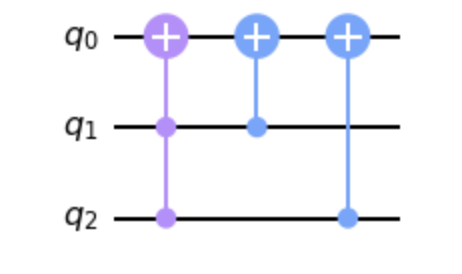
\includegraphics[scale=0.7]{reversibleOr.png}
\end{center}

\noindent This implementation was manually produced using a standard synthesis algorithm for reversible
circuits~\cite{10.1145/775832.775915}. To gain some intuition, we trace the evaluation of the circuit for input
\verb|011|. In this context, the most significant bit is at index 0. Thus the first \verb|ccx| gate negates \verb|q[0]|
since both \verb|q[1]| and \verb|q[2]| are true producing \verb|111|; the following \verb|cx| gate produces \verb|011|; finally the last \verb|cx| produces the result \verb|111|.

There is wealth of manual and algorithmic approaches for such synthesis problems each optimizing along  different dimensions~\cite{XXX}. Here is the circuit produced using an approach that analyzes the recursive structure of the circuit (and would generalize to computing the disjunction of more than two inputs):

\begin{center}
  \begin{minipage}[c]{0.4\linewidth}
\begin{verbatim}
reversibleOr2.qasm:

  // setup
  cx  q[1], q[0];
  x   q[1];
  ccx q[1], q[2], q[0];
  x   q[1];
  // measure
  \end{verbatim}
  \end{minipage}
  \qquad
  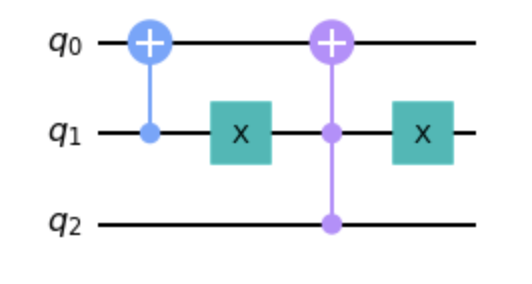
\includegraphics[scale=0.7]{reversibleOr2.png}
\end{center}

\noindent The evaluation of this circuit prints the same truth table as above confirming their equivalence. Tracing the
evaluation on the same input value \verb|011| goes through the stages \verb|111|, \verb|101|, \verb|101|, and finally \verb|111|.

The situation for Shor's algorithm is just as described above but with a more involved function of the form $f(r) = a^{r} \mod N$ for fixed $a$ and $N$. The specification of the circuit is relatively straightforward to calculate. Here it is for $a=11$ and $N=15$:
\[\begin{array}{rcll}
g(r,h) &=& \left\{ \begin{array}{ll}
                     (r,h+1) & \mbox{when~$r$~even~and~$h$~even} \\
                     (r,h-1) & \mbox{when~$r$~even~and~$h$~odd} \\
                     (r,11-h) & \mbox{when~$r$~odd~and~$4 > h \geq 0$~or~$12 > h \geq 8$} \\
                     (r,19-h) & \mbox{when~$r$~odd~and~$8 > h \geq 4$~or~$16 > h \geq 12$}
                                \end{array}\right.
\end{array}\]

\noindent However, as explained in standard accounts of the algorithm (e.g., the Qiskit implementation), producing an efficient
modular exponentiation circuit from this specification  is not straightforward and is actually the bottleneck in Shor’s algorithm. Typical
derivations of the circuit start from elementary gates, build a circuit for reversible disjunction and conjunction of
booleans, a circuit for a half-adder, a circuit for computing the carry, progressing to a circuit for modular addition,
which is used to build a circuit for modular multiplication, and then finally a circuit for modular exponentiation
taking care at each step to avoid the exponential blowup (e.g., by implementing exponentiation by squaring instead of repeated
multiplication)~\cite{shorefficient}.

\paragraph*{Our Technical Results.} The main result of the paper is a proof, formalized in the HoTT-Agda library, that
the category of finite sets and bijections is the free rig groupoid; its structure is illustrated diagrammatically below:

\[\begin{tikzcd}
    \PiLang && \PiPlusLang && \PiHatLang && \UFin
    \arrow["\evalt", from=1-1, to=1-3]
    \arrow["\evalp", curve={height=-24pt}, from=1-3, to=1-5]
    \arrow["\evalh", curve={height=-24pt}, from=1-5, to=1-7]
    \arrow["\quotep", curve={height=-24pt}, from=1-5, to=1-3]
    \arrow["\quoteh", curve={height=-24pt}, from=1-7, to=1-5]
  \end{tikzcd}\]

\noindent The nodes $\PiLang$, $\PiPlusLang$, and $\PiHatLang$ in the diagram each represent a syntactic weak 2-category
(groupoid actually as all morphisms are isomorphisms) where the 0-cells represent types, the 1-cells represent
reversible circuits, and the 2-cells represent circuit equivalences. In $\PiLang$, the circuits represent arbitrary
permutations among finite sets with products and coproducts; in $\PiPlusLang$, the circuits represent arbitrary
permutations among finite sets with only coproducts; and in $\PiHatLang$, the permutations are expressed using adjacent
transpositions.

The syntactic groupoid $\PiPlusLang$ is the free rig groupoid; $\UFin$ is the groupoid of finite sets and bijections
represented as the \emph{univalent subuniverse of all finite types}. The $\evalp/\quotep$ and $\evalh/\quoteh$ arrows
establish a \emph{symmetric monoidal biequivalence} between these two groupoids. To get a taste of the involved
complexity of this result, consider the obvious fact that, semantically, i.e., in $\UFin$, there is only one bijection
from the empty set to itself. However, in the free groupoid, there are an infinite number of isomorphisms from the empty
type to itself that go through arbitrary complex subtypes, e.g., letting $\isoone$ be the type constructor for type
isomorphisms we can have a sequence of syntactic equivalences
$\zerot \isoone \zerot \times A \isoone \zerot \times (A + \zerot) \isoone (\zerot \times A) + (\zerot \times \zerot)
\isoone (\zerot \times \zerot) + (\zerot \times A) \isoone \zerot + (\zerot \times A) \isoone \zerot + \zerot \isoone
\zerot$, and all such isomorphisms must be identified using appropriate coherence laws. The technical device to achieve
this normalization is as follows. First, we observe that 1-paths in $\UFin$ are permutations on finite sets with a fixed
cardinality $n$, given by $\Aut[\Fin[n]]$, which produce the permutation group on $\Fin[n]$, or the symmetric group
$\Sn$. By giving a presentation of $\Sn$ using generators and relations, we build a rewriting system using the Coxeter
relations~\cite{XXX} on the set of words $\List[\Fin[n]]$, and show that it is (locally) confluent and strongly
normalizing. We then establish that the symmetric group $\Sn$ is the set-quotient of $\List[\Fin[n]]$ by the Coxeter
relations, and show that it produces a group presentation, as a quotient of the free group. Using this strongly
normalizing rewriting system, we establish that normal forms for words in $\Sn$ are Lehmer
codes~\cite{lehmerTeachingCombinatorialTricks1960}, which are a convenient and compact representation of
permutations. Finally, we show that there is an equivalence between Lehmer codes and permutations $\Aut[\Fin[n]]$ given
by the Lehmer encode-decode algorithm.

Below we reduce $\mathsf{swap} : 2 + 2 \leftrightarrow 2 + 2$ to a sequence of adjacent swaps. This is an example of
a translation from $\PiPlusLang$ to $\PiHatLang$.

\begin{align*}
  \begin{tikzpicture}[scale=0.4,every node/.style={scale=0.4}]
    \begin{knot}[clip width=3]
      \filldraw (0,4) circle (2pt) node[above] {0};
      \filldraw (1,4) circle (2pt) node[above] {1};
      \filldraw (2,4) circle (2pt) node[above] {2};
      \filldraw (3,4) circle (2pt) node[above] {3};
      \filldraw (0,0) circle (2pt) node[below] {2};
      \filldraw (1,0) circle (2pt) node[below] {3};
      \filldraw (2,0) circle (2pt) node[below] {0};
      \filldraw (3,0) circle (2pt) node[below] {1};
      \strand (0,4) .. controls (0.5,1.5) and (1.5,2.5) .. (2,0);
      \strand (1,4) .. controls (1.5,1.5) and (2.5,2.5) .. (3,0);
      \strand (2,4) .. controls (1.5,1.5) and (1.5,2.5) .. (0,0);
      \strand (3,4) .. controls (2.5,1.5) and (2.5,2.5) .. (1,0);
    \end{knot}
  \end{tikzpicture}
\quad=\quad
  \begin{tikzpicture}[scale=0.4,every node/.style={scale=0.4}]
    \begin{knot}[clip width=3]
      \filldraw (0,4) circle (2pt) node[above] {0};
      \filldraw (1,4) circle (2pt) node[above] {1};
      \filldraw (2,4) circle (2pt) node[above] {2};
      \filldraw (3,4) circle (2pt) node[above] {3};
      \filldraw (0,0) circle (2pt) node[below] {0};
      \filldraw (1,0) circle (2pt) node[below] {2};
      \filldraw (2,0) circle (2pt) node[below] {1};
      \filldraw (3,0) circle (2pt) node[below] {3};
      \strand (0,4) to (0,0);
      \strand (1,4) .. controls (0.5,2) and (2.5,2) .. (2,0);
      \strand (2,4) .. controls (2.5,2) and (0.5,2) .. (1,0);
      \strand (3,4) to (3,0);
    \end{knot}
  \end{tikzpicture}
  &&
    \begin{tikzpicture}[scale=0.4,every node/.style={scale=0.4}]
      \begin{knot}[clip width=3]
        \filldraw (0,4) circle (2pt) node[above] {0};
        \filldraw (1,4) circle (2pt) node[above] {2};
        \filldraw (2,4) circle (2pt) node[above] {1};
        \filldraw (3,4) circle (2pt) node[above] {3};
        \filldraw (0,0) circle (2pt) node[below] {2};
        \filldraw (1,0) circle (2pt) node[below] {0};
        \filldraw (2,0) circle (2pt) node[below] {1};
        \filldraw (3,0) circle (2pt) node[below] {3};
        \strand (0,4) .. controls (-0.5,2) and (1.5,2) .. (1,0);
        \strand (1,4) .. controls (1.5,2) and (-0.5,2) .. (0,0);
        \strand (2,4) to (2,0);
        \strand (3,4) to (3,0);
      \end{knot}
    \end{tikzpicture}
  &&
  \begin{tikzpicture}[scale=0.4,every node/.style={scale=0.4}]
    \begin{knot}[clip width=3]
      \filldraw (0,4) circle (2pt) node[above] {2};
      \filldraw (1,4) circle (2pt) node[above] {0};
      \filldraw (2,4) circle (2pt) node[above] {1};
      \filldraw (3,4) circle (2pt) node[above] {3};
      \filldraw (0,0) circle (2pt) node[below] {2};
      \filldraw (1,0) circle (2pt) node[below] {0};
      \filldraw (2,0) circle (2pt) node[below] {3};
      \filldraw (3,0) circle (2pt) node[below] {1};
      \strand (0,4) to (0,0);
      \strand (1,4) to (1,0);
      \strand (2,4) .. controls (1.5,2) and (3.5,2) .. (3,0);
      \strand (3,4) .. controls (3.5,2) and (1.5,2) .. (2,0);
    \end{knot}
  \end{tikzpicture}
  &&
    \begin{tikzpicture}[scale=0.4,every node/.style={scale=0.4}]
      \begin{knot}[clip width=3]
        \filldraw (0,4) circle (2pt) node[above] {2};
        \filldraw (1,4) circle (2pt) node[above] {0};
        \filldraw (2,4) circle (2pt) node[above] {3};
        \filldraw (3,4) circle (2pt) node[above] {1};
        \filldraw (0,0) circle (2pt) node[below] {2};
        \filldraw (1,0) circle (2pt) node[below] {3};
        \filldraw (2,0) circle (2pt) node[below] {0};
        \filldraw (3,0) circle (2pt) node[below] {1};
        \strand (0,4) to (0,0);
        \strand (1,4) .. controls (0.5,2) and (2.5,2) .. (2,0);
        \strand (2,4) .. controls (2.5,2) and (0.5,2) .. (1,0);
        \strand (3,4) to (3,0);
      \end{knot}
    \end{tikzpicture}
\end{align*}

\note{Show codes; normalize; explain the dense paragraph above using that example}


The technical result implies several immediate applications to reversible circuits: (i) a reversible circuit expressed
in $\PiPlusLang$ can be automatically generated from a permutation in $\UFin$ \emph{and the generation comes equipped
  with a proof of correctness establishing its equivalence between the circuit and the original permutation}; (ii)
circuits in $\PiLang$ or $\PiPlusLang$ can be reduced to a circuit normal form using a normalization by evaluation
process that evaluates them to a permutation in $\UFin$ and quotes it back; (iii) equivalence of circuits in either
$\PiLang$ or $\PiPlusLang$ can be decided by reducing them to normal forms; (i) a circuit can be verified against a
given permutation by evaluating it; and (v) the induced circuit equivalences in $\PiLang$ and $\PiPlusLang$ form a sound
and complete calculus for reasoning about and optimizing circuits. (See Sec.~\ref{sec:informal} for more details.)

  \note{perhaps a note about the result being folklore; assumed in many places; but no proof; and certainly none
    formalized in a proof assistant. In some sense, what we have done is to take MacLane's coherence theorem and
    formalized it in HoTT, and given presentations for it using Pi's syntax. Also relevant is that the equivalence
    result hides implicit isomorphisms that have computational relevance. For example, transporting properties across
    equivalences of finite types can be done via executing permutations, something which has a clear computational cost
    and which itself depends on the choice of representations of the permutations.}

% \begin{itemize}[leftmargin=*]
%   \item We take the $\PiLang$ family of reversible languages~\cite{jamesInformationEffects2012} and show how to encode
%         various boolean reversible circuits in the language. The circuits are implemented using 1-combinators in the
%         language, and circuit optimisations are realized as 2-combinators between these reversible programs.
%   \item We show how to encode reversible circuits on a fixed number of bits as permutations of finite sets with the
%         appropriate cardinality. We observe that reversible programs can be translated to bijective functions between
%         finite sets and equality of reversible programs can be witnessed as extensional equality of these bijective
%         functions.
%   \item We review a few basics of Homotopy Type Theory~\cite{univalentfoundationsprogramHomotopyTypeTheory2013}, and
%         exhibit some results that we use in our technical development. We define the notion of a universe \`{a} la
%         Tarski internally in HoTT, which is given by a type for codes $U$ and a decoding function to a univalent
%         universe $\El : U \to \UU$. We say that this universe is univalent, if the decoding fibration is univalent, that
%         is, the decoding function $\El$ reflects the path space of the underlying univalent universe. We exhibit some
%         examples of univalent subuniverses, in particular, we define the subuniverse of finite types, $\UFin$, which
%         classifies all finite types, and show that it is univalent. Using this, we establish a characterization of the
%         path space of the universe of finite types.
%   \item We observe that 1-paths in $\UFin$ are permutations on finite sets with a fixed cardinality $n$, given by
%         $\Aut[\Fin[n]]$, which produces the permutation group on $\Fin[n]$, or the symmetric group $\Sn$. We then
%         proceed to give a presentation of $\Sn$ using generators and relations, by defining the Coxeter relations. We
%         build a rewriting system using the Coxeter relations on the set of words $\List[\Fin[n]]$, and show that it is
%         (locally) confluent and strongly normalising. We define the the symmetric group $\Sn$ to be the set-quotient of
%         $\List[\Fin[n]]$ by the Coxeter relations, and show that it produces a group presentation, as a quotient of the
%         free group. Using our strongly normalising rewriting system, we establish that normal forms for words in $\Sn$
%         are Lehmer codes~\cite{lehmerTeachingCombinatorialTricks1960}, which are a convenient and compact representation
%         of permutations for permutations. Finally, we show that there is an equivalence between Lehmer codes and
%         permutations $\Aut[\Fin[n]]$ given by the Lehmer encode-decode algorithm.
%   \item Finally, we show how to interpret the language $\PiLang$ into our groupoid $\UFin$, in stages. First we define a
%         subset of the language $\PiPlusLang$ which only includes the additive monoidal structure. We translate $\PiLang$
%         programs to $\PiPlusLang$ by defining multiplication as repeated addition. Then, we further define a normalized
%         form for for this language called $\PiHatLang$, which has normalized 1-combinators and 2-combinators
%         corresponding to adjacent transpositions. We show that $\PiPlusLang$ can be translated to $\PiHatLang$ and back,
%         using adjacent transpositions to generate arbitrary swaps. Then, we show how to interpret this language
%         $\PiHatLang$ into $\UFin$ -- the 1-combinators are translated into permutations via words in $\Sn$, and
%         2-combinators are interpreted as 2-paths in $\UFin$. We further show how to quote back a permutation in $\UFin$
%         into a 1-combinator using the normal form for words in $\Sn$.
%   \item We give some applications of this translation by showing how to normalise a circuit written in $\PiLang$ to a
%         normal form in $\PiPlusLang$ and $\PiHatLang$, which uses fewer gates.~\todo{Here, or earlier?}
% \end{itemize}

% Our results are formalized in the proof assistant Agda using the HoTT-Agda library.

\begin{center}
  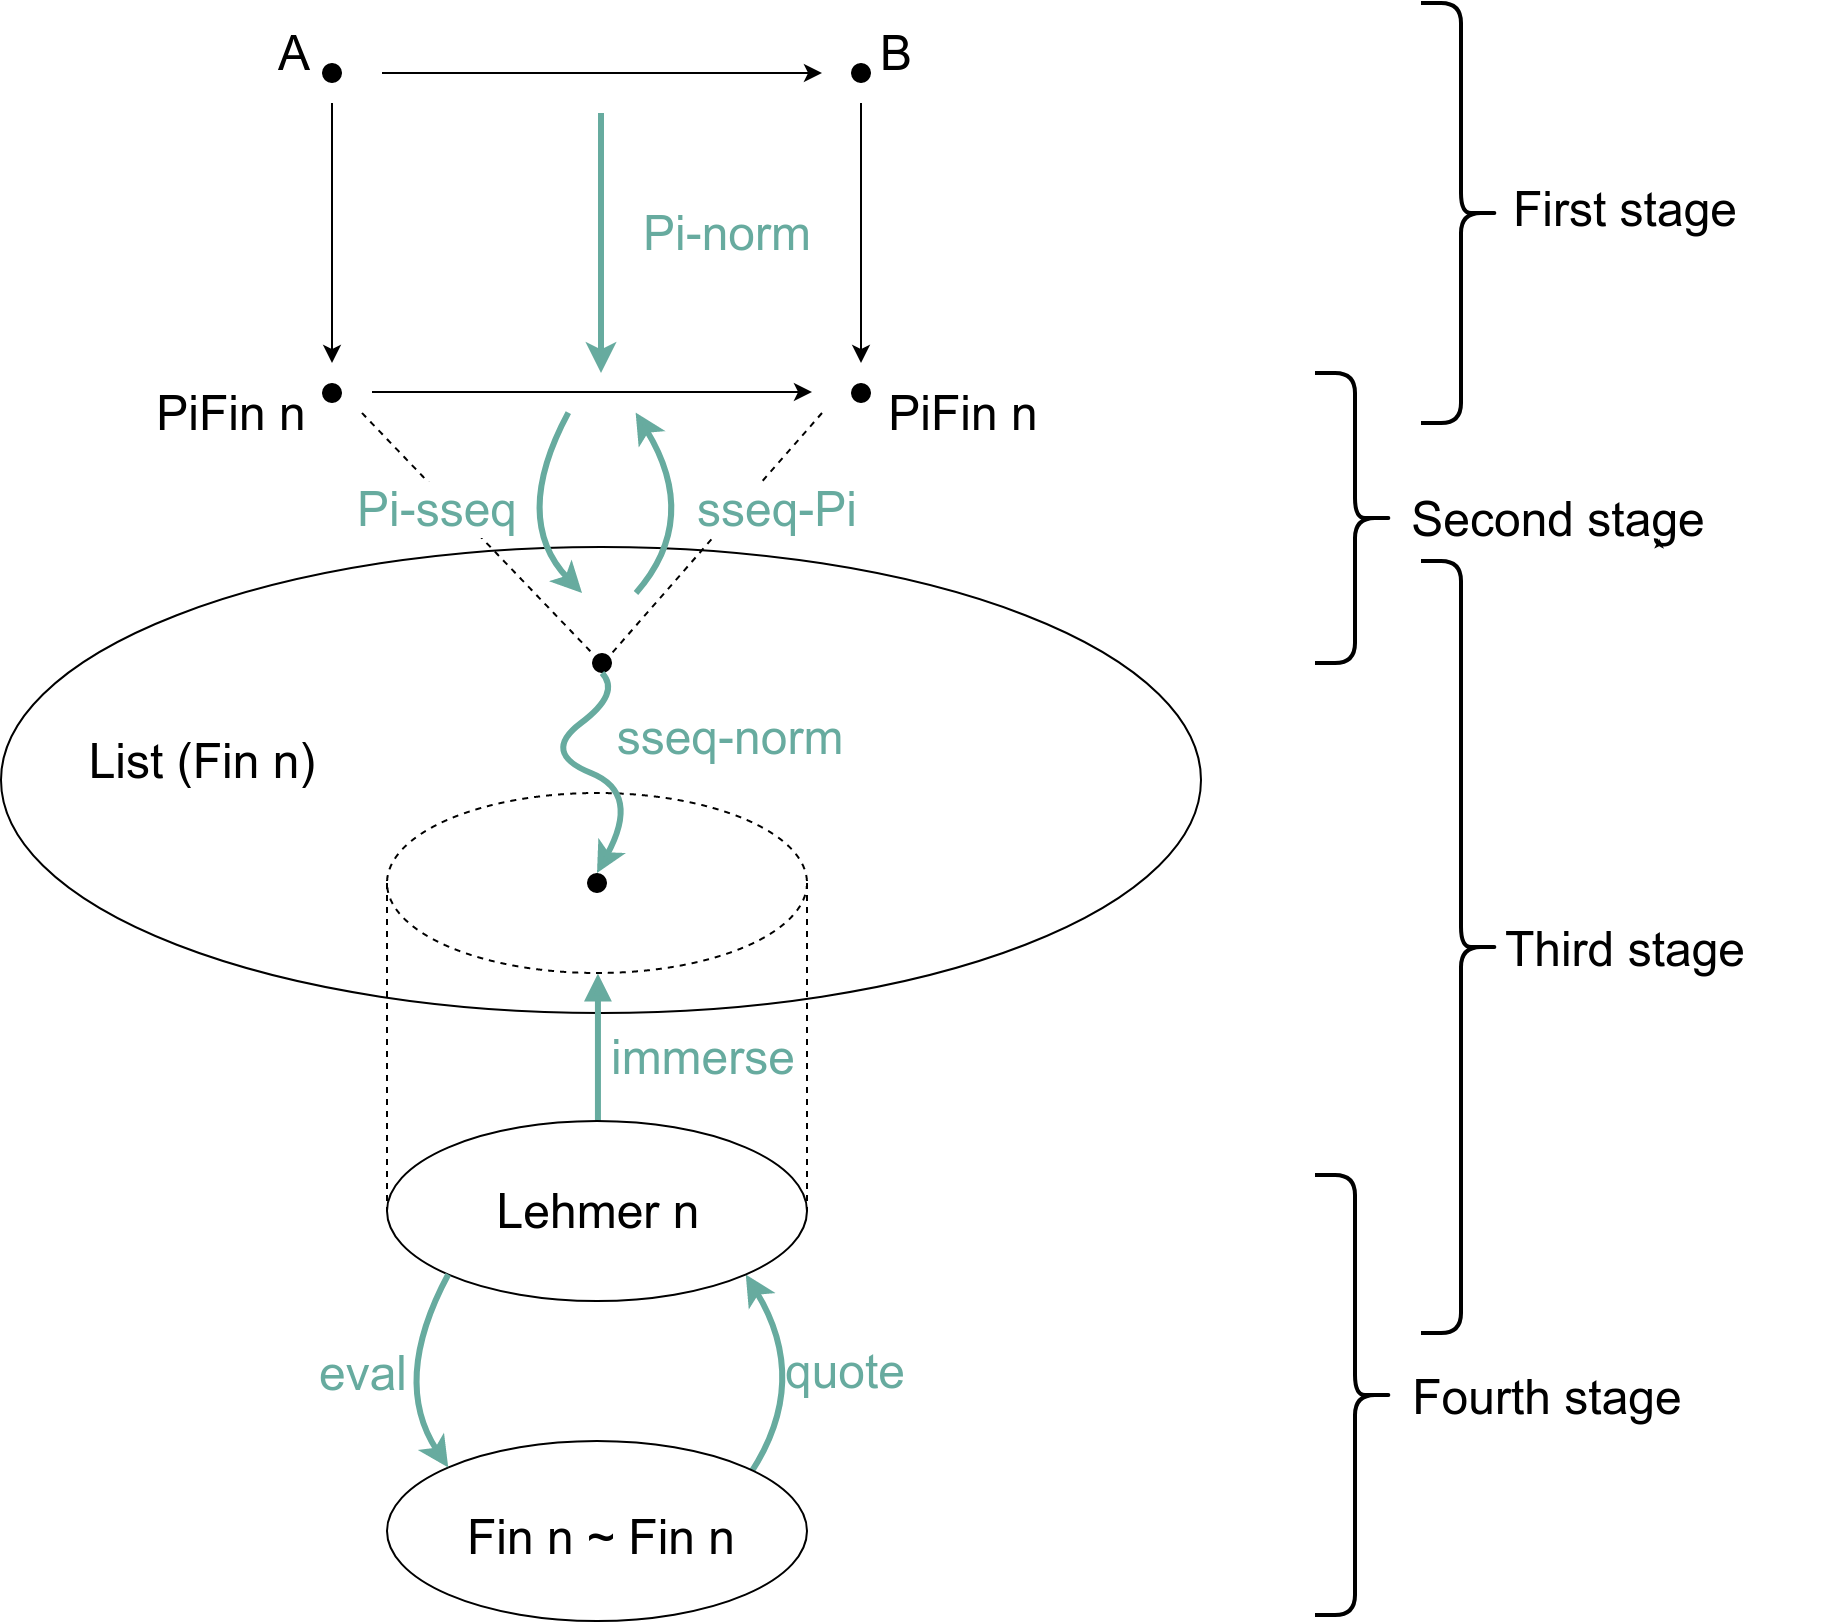
\includegraphics[scale=0.3]{outline.png}
\end{center}

\note{Redo this figure or delete ??}

\note{Spiel about reversible computing and logical reversibility ??}

\note{Spiel about using groupoids for denotational semantics ??}

\note{Could we include a short paragraph about entropy and bits and logical reversibility ??}

\note{Novel interpretation of the univalence axiom, operational and denotational semantics and adequacy.}

-------


% * STLC(first) is the type theory for CCC
%   HoTT is type theory for weak infty groupoids(first)
%   Correspondence between TT and categories are fruitful:
%   answer hard questions about syntax without worrying about presentation
%   normalization of lcal with strong sums: if you have specific syntax; no obvious induction on syntax
%   Lawvere thesis


% * Rig groupoids are interesting! WHY????
%   Add monoidal structure to weak groupoids. Easy. Lists
%   How symmetry is going to act on higher dimension
%   Higher-dim all symmetric; topology higher things abelian groups

% * What is the corresponding type theory ?
%   We give it for the free symmetric groupoid; for other groupoids build on it and add more




%%% Local Variables:
%%% mode: latex
%%% TeX-master: "main"
%%% fill-column: 120
%%% End:
                                                            % 2 pages
\section{Reversible Circuits in Qiskit}
\label{sec:qiskit}
\label{sec:examples}

Classical reversible boolean circuits are at the core of most quantum algorithms and hence are supported by popular
platforms for quantum computing such as IBM Qiskit~\cite{aleksandrowiczQiskitOpensourceFramework2019}. Specifically, the
Qiskit framework provides the following universal set of gates for reversible computing: \textsf{not} (boolean negation,
called \verb|x|), \textsf{cnot} (conditional negation of the second input if the first is true; called \verb|cx|), and
\textsf{toffoli} (conditional negation of the third input if both the first two inputs are true; called \verb|ccx|)
gates. Additionally, Qiskit allows implicit re-shuffling of bits by allowing each operation to specify the indices of
its input bits.

For concreteness, we demonstrate two different circuits that implement the
following reversible function specification
$\mathit{reversibleOr}(h,b_1,b_2) ~=~ (h \,\underline{\vee}\, (b_1 \vee b_2),
~b_1, ~b_2)$ where~$\vee$ is disjunction and~$\underline{\vee}$ is exclusive-disjunction. The circuits are presented in both the textual interface
\verb|qasm| and the graphical interface:

\medskip
\begin{tabular}{c@{\qquad}c}
\begin{minipage}[t]{0.42\linewidth}
  \begin{verbatim}
  ccx q[1], q[2], q[0];
  cx  q[1], q[0];
  cx  q[2], q[0];
  \end{verbatim}
  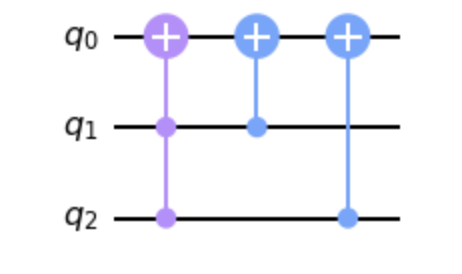
\includegraphics[scale=0.7]{reversibleOr.png}
  \end{minipage}
&
\begin{minipage}[t]{0.43\linewidth}
  \begin{verbatim}
  cx  q[1], q[0];
  x   q[1];
  ccx q[1], q[2], q[0];
  x   q[1];
  \end{verbatim}
  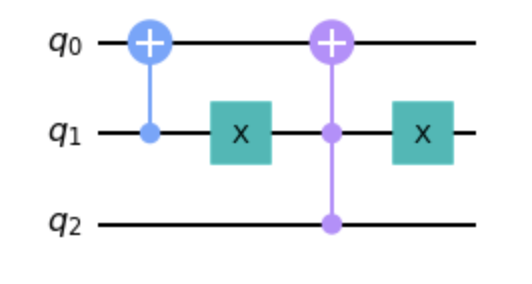
\includegraphics[scale=0.6]{reversibleOr2.png}
  \end{minipage}
\end{tabular}

\medskip

There is a wealth of manual and algorithmic approaches for producing circuits
such as the two above~\cite{maslov:2003:rls:1087512,1201583}. The circuit on the
left was manually produced using a standard synthesis algorithm for reversible
circuits~\cite{10.1145/775832.775915}. The circuit on the right was produced
using an approach that analyzes the recursive structure of
$\mathit{reversibleOr}$ (and would generalise to computing the disjunction of
more than two inputs):

From the specification of the circuit, we expect input \verb|011| to be mapped
to \verb|111|. To gain some intuition, we trace the evaluation of each circuit for
input \verb|011|. In this context, the most significant bit is at index 0. In
the first circuit, the \verb|ccx| gate negates \verb|q[0]| since both \verb|q[1]| and
\verb|q[2]| are true producing \verb|111|; the following \verb|cx| gate produces
\verb|011|; finally the last \verb|cx| produces the result \verb|111|. For the
second circuit, the trace of the execution on the same input value \verb|011| goes through the stages \verb|111|, \verb|101|, \verb|101|, and finally \verb|111|.

Although rather trivial, the examples above illustrate the general idea. A more
interesting example would be the classical core of Shor's algorithm which
requires a circuit implementing modular exponentiation $f(r) = a^{r} \mod N$ for
fixed $a$ and $N$. Using Toffoli's construction~\citeyearpar{Toffoli:1980}, a
reversible specification of this function is $f^R(r,h) = (r, f(r)
~\underline{\vee}~ h)$ where the exclusive disjunction~$\underline{\vee}$ is
applied bitwise. When $h=0$ the second component of the result of $f^R$ is the
result of the original modular exponentiation $f$.
%%
%% the specification of the circuit is relatively straightforward to
%% calculate. Here it is for $a=11$ and $N=15$:
%% \[\begin{array}{rcll}
%% g(r,h) &=& \left\{ \begin{array}{ll}
%%                      (r,h+1) & \mbox{when~$r$~even~and~$h$~even} \\
%%                      (r,h-1) & \mbox{when~$r$~even~and~$h$~odd} \\
%%                      (r,11-h) & \mbox{when~$r$~odd~and~$4 > h \geq 0$~or~$12 > h \geq 8$} \\
%%                      (r,19-h) & \mbox{when~$r$~odd~and~$8 > h \geq 4$~or~$16 > h \geq 12$}
%%                                 \end{array}\right.
%% \end{array}\]
%%
However, as explained in standard accounts of the algorithm (e.g., the
Qiskit implementation), producing an efficient modular exponentiation circuit
from this specification is not straightforward and is actually the bottleneck in
Shor’s algorithm. Typical derivations of the circuit start from elementary
gates, build a circuit for reversible disjunction (like the two circuits above),
reversible conjunction, a circuit for a half-adder, a circuit for computing the
carry, progressing to a circuit for modular addition, which is used to build a
circuit for modular multiplication, and then finally a circuit for modular
exponentiation taking care at each step to avoid the exponential blowup (e.g.,
by implementing exponentiation by squaring instead of repeated
multiplication)~\cite{shorefficient}.

% To make the connection to reversible computing explicit, we use the Agda
% formalisation of our technical result to extract various computational
% procedures to synthesise, normalise, optimise, and verify reversible
% circuits. In this introduction,

% From the definition of $\underline{\vee}$ it is evident that setting $h=0$, we can compute the desired disjunction by observing the first component of the result. The $\mathit{reversibleOr}$ function has the following truth table (in binary on the left and in a more convenient decimal notation on the right):

% \begin{center}\begin{tabular}{|ccc|ccc|@{\qquad\qquad}|c|c|}
% 0 & 0 & 0 &     0 & 0 & 0     & 0 & 0 \\
% 0 & 0 & 1 &     1 & 0 & 1     & 1 & 5 \\
% 0 & 1 & 0 &     1 & 1 & 0    & 2 & 6 \\
% 0 & 1 & 1 &     1 & 1 & 1    & 3 & 7 \\
% 1 & 0 & 0 &     1 & 0 & 0    & 4 & 4 \\
% 1 & 0 & 1 &     0 & 0 & 1    & 5 & 1 \\
% 1 & 1 & 0 &     0 & 1 & 0    & 6 & 2 \\
% 1 & 1 & 1 &     0 & 1 & 1    & 7 & 3
% \end{tabular}\end{center}

% \noindent where it is evident that it is a bijective function, i.e., reversible.

% As a simple example for that middle stage, we synthesise a reversible circuit
% implementing boolean disjunction ($\vee$). Following~\citet{Toffoli:1980}, the
% first step is to write a specification for the desired reversible function:

% The above embedding of an irreversible function into a reversible function with
% additional inputs and outputs is completely general and is the starting point
% for specifications of quantum circuits. The challenge is to synthesise a program
% / circuit from this specification. Of course, writing this program in a
% conventional (irreversible) language defeats the purpose. The challenge is to
% construct the desired program / circuit exclusively using reversible primitives,
% e.g.,

% the standard set of universal reversible gates used in frameworks like
% Qiskit which consists of the computational gates \textsf{not} (boolean negation,
% called \verb|x|), \textsf{cnot} (conditional negation of the second input if the
% first is true; called \verb|cx|), and \textsf{toffoli} (conditional negation of
% the third input if both the first two inputs are true; called \verb|ccx|) gates,
% and the ability re-arrange the layout of wires.
 % sec 1.5                                          % 2 pages
\begin{figure}[t]
  {\scalebox{\scalef}{$%
        %%\noindent\begin{minipage}{.7\linewidth}
        \begin{array}{rrcll}
          \idc :     & A                     & \isoone & A                            & : \idc      \\
          \\
          \identlp : & \zerot + A            & \isoone & A                            & : \identrp  \\
          \swapp :   & A + B                 & \isoone & B + A                        & : \swapp    \\
          \assoclp : & A + (B + C)           & \isoone & (A + B) + C                  & : \assocrp  \\ [1.5ex]
          \identlt : & \onet \times A        & \isoone & A                            & : \identrt  \\
          \swapt :   & A \times B            & \isoone & B \times A                   & : \swapt    \\
          \assoclt : & A \times (B \times C) & \isoone & (A \times B) \times C        & : \assocrt  \\ [1.5ex]
          \absorbr : & ~ \zerot \times A     & \isoone & \zerot ~                     & : \factorzl \\
          \dist :    & ~ (A + B) \times C    & \isoone & (A \times C) + (B \times C)~ & : \factor
        \end{array}$}}

  \medskip

  {\scalebox{\scalef}{%
      \Rule{}
      {\jdg{}{}{c_1 : A \isoone B} \quad \vdash c_2 : B \isoone C}
      {\jdg{}{}{c_1 \fatsemi c_2 : A \isoone C}}
      {}

      \Rule{}
      {\jdg{}{}{c_1 : A \isoone B} \quad \vdash c_2 : C \isoone D}
      {\jdg{}{}{c_1 \oplus c_2 : A + C \isoone B + D}}
      {}

      \Rule{}
      {\jdg{}{}{c_1 : A \isoone B} \quad \vdash c_2 : C \isoone D}
      {\jdg{}{}{c_1 \otimes c_2 : A \times C \isoone B \times D}}
      {}
    }}
  \caption{$\Pi$-terms, combinators, and their types.}
  \label{fig:pi-terms}
\end{figure}

\section{A Reversible Programming Language}
%% ~3 pages
\label{sec:pi}
\label{sec:reversibleone}
\label{sec:reversibletwo}
\label{langeqeq}
\label{sec:informal}

The circuit model of reversible computation discussed in the previous section is a useful abstraction close to the hardware
platform. However, since its main data abstraction is a \emph{sequence of wires}, it only provides an ``assembly-level''
programming abstraction (e.g., \verb|qasm|). As motivated by \citet{LAFONT2003257}, a mathematical model based on
permutations of finite sets provides a richer algebraic structure which we review in this section.

%%%%%%%%%%%%%%%%%
\subsection{The $\Pi$ Family of Languages}
\label{sec:langRev-examples}
\label{examples}

In a reversible boolean circuit, the number of input bits matches the number of output bits. Circuits can be composed
sequentially, vertically, or horizontally, respectively preserving the number of bits, adding up the number of bits or
multiplying them. So, to program with reversible circuits, all we need to do is make sure that each primitive operation
preserves the number of bits, which is just a natural number. Natural numbers are the free commutative semiring (or,
commutative rig) on one generator, with $(0,+)$ for addition, and $(1,\times)$ for multiplication, so the commutative
semirig identities can be used to design a logic for reversible programming. This inspired the syntax for various
first-order reversible logics and reversible programming
languages~\cite*{sparksSuperstructuralReversibleLogic2014,jamesInformationEffects2012}.

Natural number identities have no computational content. To obtain a computational interpretation of the commutative rig
structure, the logic needs to be equipped with values and types, and a notion of operational semantics and contextual
equivalence~\cite{jamesInformationEffects2012}. This is a programming language which embodies the computational content
of isomorphisms of finite types, or permutations. On the semantic side, we need to consider the groupoidification of a
commutative rig, that is, a symmetric rig groupoid. A sound semantics for $\PiLang$ in weak rig groupoids was
established in~\cite{caretteComputingSemiringsWeak2016}, and conjectured to be complete.

% In programming parlance, as shown in~\cref{fig:pi-terms}, each primitive algebraic identity of commutative rigs becomes
% a reversible combinator in the programming language and the algebraic closure operators become composition operators in
% the programming language. Once equipped with a notion of values and types, we get the following syntactic presentation
% of a programming language for permutations~\cite{James:2012:IE:2103656.2103667,Carette2016}:

% A specialised language for programming with permutations on finite sets can be built using ideas going back to Kelly,
% Laplaza, and Mac Lane~\cite{laplaza72,kelly74,KELLY197197} that the commutative semiring (also known as the commutative
% rig) of natural numbers exactly characterizes permutations on finite sets. In programming parlance, as shown in
% Fig.~\ref{fig:pi-terms}, each primitive algebraic identity of commutative rigs becomes a constant in the programming
% language and the algebraic closure operators become composition operators in the programming language. Once equipped
% with a notion of values and types, we get the following syntactic presentation of a programming language for
% permutations~\cite{James:2012:IE:2103656.2103667,Carette2016}:

% The practice of programming languages is replete with \emph{ad hoc} instances of reversible computations: database
% transactions, mechanisms for data provenance, checkpoints, stack and exception traces, logs, backups, rollback
% recoveries, version control systems, reverse engineering, software transactional memories, continuations, backtracking
% search, and multiple-level undo features in commercial applications. In the early nineties,
% \citet{Baker:1992:LLL,Baker:1992:NFT} argued for a systematic, first-class, treatment of reversibility. But intensive
% research in full-fledged reversible models of computations and reversible programming languages was only sparked by the
% discovery of deep connections between physics and
% computation~\cite{Landauer:1961,PhysRevA.32.3266,Toffoli:1980,bennett1985fundamental,Frank:1999:REC:930275, Hey:1999:FCE:304763,fredkin1982conservative}, and by the
% potential for efficient quantum computation~\cite{springerlink:10.1007/BF02650179}.

% The early developments of reversible programming languages started
% with a conventional programming language, e.g., an extended
% $\lambda$-calculus, and either:
% \begin{enumerate}
%   \item extended the language with a history
%         mechanism~\cite{vanTonder:2004,Kluge:1999:SEMCD,lorenz,danos2004reversible}, or
%   \item imposed constraints on the control flow constructs to make them
%         reversible~\cite{Yokoyama:2007:RPL:1244381.1244404}.
% \end{enumerate}
% More foundational approaches recognize that reversible programming languages require a fresh approach and should be
% designed from first principles without the detour via conventional irreversible
% languages~\cite{Yokoyama:2008:PRP,Mu:2004:ILRC,abramsky2005structural,DiPierro:2006:RCL:1166042.1166047,
%   rc2011, James:2012:IE:2103656.2103667, Carette2016}.

\medskip

{\scalebox{\scalef}{$%
      \begin{array}{lrcl}
        \textit{Value types}   & A,B,C,D & ::= & \zerot \alt \onet \alt A+B \alt A\times B        \\
        \textit{Values}        & v,w,x,y & ::= & \Acon{tt} \alt \inlv{v} \alt \inrv{v} \alt (v,w) \\
        \textit{Program types} &         &     & A \isoone B                                      \\
        \textit{Programs}      & c       & ::= & (\textrm{See Fig.~\ref{fig:pi-terms}})
      \end{array}$}}

\medskip\noindent The language of types is built from the empty type ($\zerot$), the unit type
($\onet$) containing just one value~$\Acon{tt}$, the sum type ($+$) containing values of the form $\inlv{v}$ and
$\inrv{v}$, and the product type ($\times$) containing pairs of values $(v_1,v_2)$.
%
% A natural candidate for a semantic foundation for reversible programming languages is the notion of type
% isomorphism. Indeed, the type isomorphisms among finite types are sound and complete for all permutations on finite
% types~\cite{Fiore:2004,fiore-remarks} and hence they are \emph{complete} for expressing reversible combinational
% circuits~\cite{fredkin1982conservative, James:2012:IE:2103656.2103667,Toffoli:1980} and the extension with recursive
% types and trace operators~\cite{Hasegawa:1997:RCS:645893.671607} is a Turing-complete reversible
% language~\cite{James:2012:IE:2103656.2103667,rc2011}.

To see how this language expresses reversible circuits, we present a few examples. First it is possible to directly
mimic the \verb|qasm|-perspective by defining types that describe sequences of booleans. We use the type
$\mathbb{2} = \onet + \onet$ to represent booleans with $\inlv{\Acon{tt}}$ representing \textsf{true} and
$\inrv{\Acon{tt}}$ representing $\textsf{false}$. Boolean negation (the \verb|x|-gate) is straightforward to define using
the primitive combinator $\swapp$. We can represent $n$-bit words using an n-ary product of boolean values, thus the
type $\mathbb{2} \times (\mathbb{2} \times \mathbb{2})$ (abbreviated $\mathbb{B}~3$) corresponds to a collection of
wires that can transmit three bits.
%
% For example, we can express a 3-bit word reversal operation as follows:
% $\Afun{reverse} : \mathbb{B}~3 \iso \mathbb{B}~3$
% $\Afun{reverse} = \swapt \fatsemi (\swapt  \otimes  \idc)~ \fatsemi \assocrt$
% \noindent The manual trace of $\Afun{reverse}$ below confirms that it indeed reverses the three bits:
% \[\begin{array}{rlr}
%                          & (v_1, (v_2, v_3)) \\
%     \swapt               & ((v_2, v_3), v_1) \\
%     \swapt \otimes  \idc & ((v_3, v_2), v_1) \\
%     \assocrt             & (v_3, (v_2, v_1)) \\
%   \end{array}\]
%subcode source isomorphisms.tex:979
%
To express the \verb|cx| and \verb|ccx| gates, we need to encode a notion of conditional expression. Such conditionals
turn out to be expressible using the distributivity and factoring identities of rigs as shown below:

\medskip

\cif{}

\noindent The input value of type $\mathbb{2} \times A$ is processed by the distribute operator \ensuremath{\dist},
which converts it into a value of type $(\onet \times A) + (\onet \times A)$. In the left branch, which corresponds to
the case when the boolean is \textsf{true}, the combinator~\ensuremath{c_1} is applied to the value of
type~\ensuremath{A}. The right branch which corresponds to the boolean being \textsf{false} passes the value of type $A$
through the combinator \ensuremath{c_2}.  The inverse of \ensuremath{\dist}, namely \ensuremath{\factor} is applied to
get the final result. Using this conditional operator, \verb|cx| is defined as $\Afun{cif}~\verb|x|~\idc$ and
\verb|ccx| is defined as $\Afun{cif}~\verb|cx|~\idc$. With these conventions, the first circuit in the introduction
is transcribed as follows:

\medskip

\adder{}

\noindent where we clearly see the sequences of the three operations \verb|ccx|, \verb|cx|, and \verb|cx| but, instead
of using the indices in the sequence of wires to identify the relevant parameters, here we use structural isomorphisms
(elided above) to re-shuffle the types. For the second circuit, instead of transcribing it directly, we express it using
a slightly more abstract notation:

\medskip

\resettwo{}

\noindent Like the original circuit, we examine the bit at index 1 (corresponding to the component $B$ in a tuple
$(A,(B,C))$): if the bit is true, we perform an \verb|x| operation on component $A$, and otherwise we perform a
\verb|cx| operation on $(C,A)$. The two uses of \verb|x| gates in the circuit are now unnecessary as they were only needed
to encode a two-way conditional expression using a sequence of one-way conditional expressions (the only ones available in
the linear circuit model).

All of this is only half the story however as the correspondence between the syntactic commutative rig (the syntax of $\PiLang$)
and permutations on finite sets includes \emph{coherence conditions} that identify different syntactic representations
of the same permutation~\cite{laplaza72,Carette2016}. These coherence conditions are collected in a second level of $\PiLang$
syntax as level-2 combinators whose types are of the form $c_1 \isotwo c_2$ for appropriate $c_1$ and $c_2$ of the same
level-1 type $A \isoone B$. For example, we have:

\medskip

\combtwo{}

\noindent where the first level-2 combinator states the obvious fact that compositions with the identity can be
optimized and the second level-2 combinator states the more interesting observation that swapping the two sides of a sum
type and then applying $c_1$ to the left and $c_2$ to the right is equivalent to applying $c_2$ to the left and $c_1$ to
the right and then swapping. The full set of level-2 combinators is large and is only listed in the accompanying code.

% and that impose various coherence conditions on the level-1 combinators. In the remainder of this section, we show how
% to use a subset of these level-2 combinators to show the equivalence of \Afun{reversibleOr1} and \Afun{reversibleOr2}.

% \medskip

% \orequiv{}

% \note{This section should explain the main technical parts of the paper
%   informally, without using any technology. Use an example, such as, a
%   reversible language with $\leq 5$ bits, and examples of permutations and
%   transpositions, and when they're equal.}

%%%%%%%%%
\subsection{Denotational Semantics}
\label{subsec:denotational}

\noindent The accompanying code includes an operational semantics for $\Pi$. A denotational semantics can be specified
by mapping each type to a finite set and each combinator to a permutation between finite sets. In this section, we
outline a simple denotational semantics expressed in the metalanguage of sets and functions that collapses the level-2
combinators. This semantics will be extended in the next two sections to the HoTT metalanguage to properly model the
level-2 combinators.

The denotation of types is straightforward:

\begin{center}
  {\scalebox{\scalef}{$%
        \begin{array}{rcl}
          \denot{\zerot}     & = & \bot                       \\
          \denot{\onet}      & = & \top                       \\
          \denot{A + B}      & = & \denot{A} \sqcup \denot{B} \\
          \denot{A \times B} & = & \denot{A} \times \denot{B}
        \end{array}$}}
\end{center}

\noindent where $\bot$ is the empty set, $\top$ is a singleton set, $\sqcup$ is the disjoint union of sets, and $\times$
is the cartesian product of sets. The denotation of a combinator $c : A \isoone B$ is a (bijective) function mapping
$\denot{A}$ to $\denot{B}$:

\begin{multicols}{2}
  %%  \begin{longtable}{>{$}r<{$} >{$}l<{$} >{$}c<{$} >{$}l<{$}}
  {\scalebox{\scalef}{$%
        \begin{array}[t]{rlcl}
          \denot{\identlp} & (\inl{v})         & = & v               \\
          \denot{\identrp} & v                 & = & \inl{v}         \\
          \denot{\swapp}   & (\inl{v})         & = & \inr{v}         \\
          \denot{\swapp}   & (\inr{v})         & = & \inl{v}         \\
          \denot{\assoclp} & (\inl{v})         & = & \inl{(\inl{v})} \\
          \denot{\assoclp} & (\inr{(\inl{v})}) & = & \inl{(\inr{v})} \\
          \denot{\assoclp} & (\inr{(\inr{v})}) & = & \inr{v}         \\
          \denot{\assocrp} & (\inl{(\inl{v})}) & = & \inl{v}         \\
          \denot{\assocrp} & (\inl{(\inr{v})}) & = & \inr{(\inl{v})} \\
          \denot{\assocrp} & (\inr{v})         & = & \inr{(\inr{v})}
        \end{array}$}}

  {\scalebox{\scalef}{$%
        \begin{array}[t]{rlcl}
          \denot{\identlt} & (\ttt , v)          & = & v                   \\
          \denot{\identrt} & v                   & = & (\ttt , v)          \\
          \denot{\swapt}   & (v_1 , v_2)         & = & (v_2 , v_1)         \\
          \denot{\assoclt} & (v_1 , (v_2 , v_3)) & = & ((v_1 , v_2) , v_3) \\
          \denot{\assocrt} & ((v_1 , v_2) , v_3) & = & (v_1 , (v_2 , v_3)) \\
          \denot{\dist}    & (\inl{v_1} , v_3)   & = & \inl{(v_1 , v_3)}   \\
          \denot{\dist}    & (\inr{v_2 , v_3})   & = & \inr{(v_2 , v_3)}   \\
          \denot{\factor}  & (\inl{(v_1 , v_3)}) & = & (\inl{v_1} , v_3)   \\
          \denot{\factor}  & (\inr{(v_2 , v_3)}) & = & (\inr{v_2} , v_3)
        \end{array}$}}

  %%\end{longtable}
\end{multicols}

\begin{center}
  {\scalebox{\scalef}{$%
        \begin{array}{rlcl}
          \denot{\idc}               & v           & = & v                                   \\
          \denot{(c_1 \fatsemi c_2)} & v           & = & (\denot{c_2} \circ \denot{c_1}) v   \\
          \denot{(c_1 \oplus c_2)}   & (\inl{v})   & = & \inl{(\denot{c_1}~v)}               \\
          \denot{(c_1 \oplus c_2)}   & (\inr{v})   & = & \inr{(\denot{c_2}~v)}               \\
          \denot{(c_1 \otimes c_2)}  & (v_1 , v_2) & = & (\denot{c_1} v_1 , \denot{c_2} v_2)
        \end{array}
      $}}
\end{center}

% \begingroup
% \allowdisplaybreaks
% \begin{align*}
% \end{align*}
% \endgroup

% \begin{center}
% \begin{tikzpicture}[scale=0.7,every node/.style={scale=0.8}]
%   \draw[>=latex,<->,double,red,thick] (2.25,-1.2) -- (2.25,-2.9) ;
%   \draw[fill] (-2,-1.5) circle [radius=0.025];
%   \node[below] at (-2.1,-1.5) {$A$};
%   \node[below] at (-2.1,-1.9) {$+$};
%   \draw[fill] (-2,-2.5) circle [radius=0.025];
%   \node[below] at (-2.1,-2.5) {$B$};

%   \draw[fill] (6.5,-1.5) circle [radius=0.025];
%   \node[below] at (6.7,-1.5) {$C$};
%   \node[below] at (6.7,-1.9) {$+$};
%   \draw[fill] (6.5,-2.5) circle [radius=0.025];
%   \node[below] at (6.7,-2.5) {$D$};

%   \draw[<-] (-2,-1.5) to[bend left] (1,0.5) ;
%   \draw[<-] (-2,-2.5) to[bend left] (1,-0.5) ;
%   \draw[->] (3.5,0.5) to[bend left] (6.5,-1.45) ;
%   \draw[->] (3.5,-0.5) to[bend left] (6.5,-2.45) ;

%   \draw[<-] (-2,-1.5) to[bend right] (1,-3.5) ;
%   \draw[<-] (-2,-2.5) to[bend right] (1,-4.5) ;
%   \draw[->] (3.5,-3.5) to[bend right] (6.5,-1.55) ;
%   \draw[->] (3.5,-4.5) to[bend right] (6.5,-2.55) ;


%   \draw     (2,0.5)  -- (2.5,0.5)  ;
%   \draw     (2,-0.5) -- (2.5,-0.5) ;

%   \draw     (2.5,0.5)  -- (3.5,-0.5)  ;
%   \draw     (2.5,-0.5) -- (3.5,0.5) ;

%   \draw     (1,-3.5)  -- (2,-4.5)    ;
%   \draw     (1,-4.5) -- (2,-3.5)   ;

%   \draw     (2,-3.5)  -- (2.5,-3.5)    ;
%   \draw     (2,-4.5) -- (2.5,-4.5)   ;

%   \path (1.5,0.5) node (tc1) [func] {$c_1$};
%   \path (1.5,-0.5) node (tc2) [func] {$c_2$};
%   \path (3,-4.5) node (bc1) [func] {$c_1$};
%   \path (3,-3.5) node (bc2) [func] {$c_2$};
% \end{tikzpicture}
% \end{center}
% The top path is the $\Pi$ program $(c_1~\oplus~c_2)~\odot~\swapp$ which acts on the type $A$ by $c_1$, acts on the type
% $B$ by $c_2$, and acts on the resulting value by a twist that exchanges the two injections into the sum type. The bottom
% path performs the twist first and then acts on the type $A$ by $c_1$ and on the type $B$ by $c_2$ as before. One could
% imagine the paths are physical \emph{elastic} wires in $3$ space, where the programs $c_1$ and $c_2$ as arbitrary
% deformations on these wires, and the twists do not touch but are in fact well-separated. Then, holding the points $A$,
% $B$, $C$, and $D$ fixed, it is possible to imagine sliding $c_1$ and $c_2$ from the top wire rightward past the twist,
% and then using the elasticity of the wires, pull the twist back to line up with that of the bottom --- thus making both
% parts of the diagram identical.  Each of these moves can be undone (reversed), and doing so would take the bottom part
% of the diagram into the top part.  In other words, there exists an equivalence of the program
% $(c_1~\oplus~c_2)~\odot~\swapp$ to the program $\swapp \odot (c_2~\oplus~c_1)$. We can also show that this means that,
% as permutations, $(c_1~\oplus~c_2)~\odot~\swapp$ and $\swapp \odot (c_2~\oplus~c_1)$ are equal. And, of course, not all
% programs between the same types can be deformed into one another. The simplest example of inequivalent deformations are
% the two automorphisms of $1+1$, namely $\idc$ and $\swapp$.

% The denotational semantics can be used to evaluate programs and to check equivalence of programs. For example, it is
% straightforward to verify that $\denot{(c_1~\oplus~c_2)~\fatsemi~\swapp} = \denot{\swapp \fatsemi (c_2~\oplus~c_1)}$. A
% slightly more involved example are the following two programs:

% \rotate{}

% \noindent The first program performs the following sequence of transformations:
% \[
%   \Tree [ {\small a} [ {\small b} {\small c} ] ] ~\to~
%   \Tree [ [ {\small a} {\small b} ] {\small c} ] ~\to~
%   \Tree [ {\small c} [ {\small a} {\small b} ] ] ~\to~
%   \Tree [ {\small c} [ {\small b} {\small a} ] ] ~.
% \]
% \noindent
% while the second evaluates as follows:
% \[
%   \Tree [ {\small a} [ {\small b} {\small c} ] ] ~\to~
%   \Tree [ {\small a} [ {\small c} {\small b} ] ] ~\to~
%   \Tree [ [ {\small a} {\small c} ] {\small b} ] ~\to~
%   \Tree [ [ {\small c} {\small a} ] {\small b} ] ~\to~
%   \Tree [ {\small c} [ {\small a} {\small b} ] ] ~\to~
%   \Tree [ {\small c} [ {\small b} {\small a} ] ] ~.
% \]

% The semantics above can be packaged in the category of finite sets and functions, $\SetFin$, which is the category
% freely generated by finite coproduct completion of the terminal category. Objects of $\SetFin$ can be identified with
% sets of fixed cardinality, that is, $\Fin[n] \defeq \Set{0,1,\ldots,n-1}$. $\SetFin$ has finite coproducts and products,
% which lets us interpret the types of $\PiLang$. Combinators are interpreted as morphisms in $\SetFin$, but we have to
% restrict to invertible morphisms, that is, isomorphisms. This gives the \emph{groupoid} of finite sets and bijections,
% $\BFin \defeq \mathsf{core}(\SetFin)$. The isomorphisms satisfied by coproducts and products in $\SetFin$ lift to
% $\BFin$, but they're no longer categorical coproducts and products. They give two symmetric monoidal tensor products on
% $\BFin$, the additive and multiplicative ones, with the multiplicative tensor distributing over the additive tensor.

% \note{change thm:
%   1. Each function is a bijection. 2. If there is a 2-combinator, the denotations of the 1-combinators are equal
% }

\begin{theorem}\label{thm:semone}
  The denotational semantics is sound in the following sense:
  \begin{itemize}
    \item For every level-1 combinator $c : A \isoone B$, we have that $\denot{c}$ is a bijection between $\denot{A}$ and $\denot{B}$.
    \item For every pair of combinators $c_1$ and $c_2$ of the same type $A \isoone B$, if there exists a level-2
          combinator $\alpha$ such that $\alpha : c_1 \isotwo c_2$, then $\denot{c_1} = \denot{c_2}$ using
          extensional equivalence of functions.
  \end{itemize}
\end{theorem}
\begin{proof}
  For every primitive combinator $c$ listed on one side of Fig.~\ref{fig:pi-terms}, let $!c$ be the combinator listed on
  the other side. Thus $! \assoclp$ is $\assocrp$ and $! \swapp$ is $\swapp$ itself. Then we have that $\denot{c}$ and
  $\denot{!c}$ form an equivalence. For the level-2 combinator \Afun{idr◎l}, we check
  $\denot{\AgdaBound{c}~\AgdaOperator{\AgdaInductiveConstructor{◎}}~\AgdaInductiveConstructor{id⟷₁}}
    = \mathit{id} \circ \denot{c} = \denot{c}$. The other cases are only slightly more involved calculations.
\end{proof}


%   Let $\sim$ be the following equivalence relation on combinators $c_1 \sim c_2$ iff $\denot{c_1} = \denot{c_2}$
%   identifying combinators with the same denotation.  The notation $[c]_{\sim}$ refers to a representative combinator
%   from a $\sim$-equivalence class. Using this relation, we define the
%   category $\mathcal{C}$ as follows:
%   \begin{itemize}
%     \item $\mathit{Obj}(\mathcal{C})$ is the set of $\Pi$-types, and
%     \item $\mathit{Hom}(A,B) = [c : A \isot B]_{\sim}$
%   \end{itemize}
%   The category $\mathcal{C}$ is a groupoid.
% \end{theorem}
% \begin{proof}
%   The relation $\sim$ identifies $c$, $\idc \circ c$, and $c \circ \idc$, and is associative. Furthermore, the denotation
%   of each combinator is a reversible function thus making every morphism into an isomorphism.
% \end{proof}

% \note{Then say that $\mathcal{C}$ is ``the same'' as $\BFin$ We can say here that the relation $\sim$ also identifies
%   $(c_1~\oplus~c_2)~\fatsemi~\swapp$ and $\swapp \fatsemi (c_2~\oplus~c_1)$ and other properties. ?? }

% \[\begin{array}{l}
%     \Tree[ {\small a} [ {\small b} {\small c} ] ] \\
%     2 \quad 1 \quad 0 \\
%     0 \quad 2 \quad 1 \\
%     \Tree[ [ {\small b}  {\small c} ] {\small a} ]
% \end{array}\]

% Such functions are finitely supported, that is, their outputs can be tabulated using the canonical ordering on
% $\Fin[n]$. For bijections, this gives a listed permutation. By observing the action of the combinators on the values of
% the finite set, we can define a denotational semantics which constructs the bijection.
% \note{\(\Fin[n] \to A \eqv <\type{Vec_{n}}(A)\)}

% In the previous section, we examined equivalences between conventional data structures, i.e., structured trees of
% values. We now consider a richer but foundational notion of data: programs themselves. Indeed, universal computation
% models crucially rely on the fact that \emph{programs are (or can be encoded as) data}, e.g., a Turing machine can be
% encoded as a string that another Turing machine (or even the same machine) can manipulate. Similarly, first-class
% functions are the \emph{only} values in the $\lambda$-calculus.  In our setting, we ask whether the programs developed
% in the previous section can themselves be subject to (higher-level) equivalences?

Using categorical language, the denotational semantics for $\PiLang$ is using the category of finite sets and functions
$\SetFin$. However, we only use the bijective functions for the semantics, which means, we use the groupoid $\BFin =
  \term{core}(\SetFin)$ of finite sets and bijections. $\SetFin$ has finite coproducts $(\emptyt, \sqcup)$ and finite
products $(\unit, \times)$, which we use to interpret our types. In $\BFin$, the coproducts and products restrict to
additive and multiplicative symmetric monoidal structures, respectively, making $\BFin$ a symmetric rig groupoid.

%%% Local Variables:
%%% mode: latex
%%% TeX-master: "main"
%%% fill-column: 120
%%% End:
 % sec 2 front                                         % 2 pages
\section{The Groupoid of Finite Types}
\label{sec:ufin}

The denotational semantics for $\PiLang$ in the previous section forms a groupoid $\BFin$ whose objects are finite sets
and whose (iso)morphisms as bijections between finite sets. The semantics interprets types as objects in~$\BFin$,
1-combinators as isomorphisms in~$\BFin$, and for every pair of 1-combinators related by a 2-combinator, their
interpretations are extensionally equal in~$\BFin$. In other words, this groupoid is strict: two equal permutations are
extensionally identified, without an explicit witness for the equality. In order to establish completeness, we want to
quote back from the semantics to the syntax. Specifically, given a morphism in $\BFin$, we want to produce a
1-combinator in $\PiLang$, and given two extensionally equal morphisms in $\BFin$, we want to produce a 2-combinator
witnessing the equality of the quoted 1-combinators. Our first step is therefore to \emph{weaken} this groupoid $\BFin$
by replacing the equational axioms of the category by higher invertible cells. In a weak category, the identity and
associativity equational conditions are replaced by higher invertible cells for the left and right units of composition
and for associativity; these higher cells come with their own coherence data as well, such as vertical composition, and
horizontal composition, or whiskering as detailed in Appendix~\ref{app:twocat}.

HoTT provides a rich internal language for working with weak higher groupoids, using the ``types are weak
$\infty$-groupoids'' correspondence. In this section, we show that the weakened version of the groupoid $\BFin$ can be
written in HoTT as a type $\UFin$, which is a 1-groupoid that has points for 0-cells, 1-paths for 1-cells, 2-paths for
2-cells with at most one 2-cell between compatible 1-cells.

%% In this section, we develop the tools necessary to construct $\UFin$, starting with a quick review of HoTT.
%% Using the identity type for morphisms, a 1-groupoid in HoTT

IS THAT FOOTNOTE NECESSARY ??? We should avoid using footnotes as much as possible.\footnote{This is a locally-strict
  $(2,0)$-category, since every cell above 0 is invertible, and the hom-categories are posets, that is, truth-value
  enriched.}

\begin{toappendix}
  We give an example of the groupoid structure on a 3-element set.

  \[
    \begin{tikzcd}
      \Fin[3]
      \arrow[""{name=0, anchor=center, inner sep=0}, "{f_{3}}", no head, loop, distance=4em, in=115, out=65]
      \arrow[""{name=0, anchor=center, inner sep=0}, "{f_{2}}", no head, loop, distance=8em, in=125, out=55]
      \arrow[""{name=1, anchor=center, inner sep=0}, "{f_{1}}"', no head, loop, distance=12em, in=135, out=45]
      \arrow["", "{h}", shorten <=3pt, shorten >=3pt, Rightarrow, no head, from=0, to=1]
    \end{tikzcd}
  \]

  We have $\Fin[3] = \Set{0,1,2} \eqv \unit \sqcup (\unit \sqcup \unit)$ which fixes a particular enumeration of the
  elements. Suppose we have a set $X = (\unit \sqcup \unit) \sqcup \unit$, it has the same cardinality as $\Fin[3]$, so it
  is represented by the same 0-cell. But, $X$ can be made equivalent to $\Fin[3]$ in many different ways since there are
  many bijections between them. One bijection is
  $\Set{\inl(\inl(\ttt)) \mapsto 0, \inl(\inr(\ttt)) \mapsto 1, \inr(\ttt) \mapsto 2}$ which can be written in two
  different ways by composing more primitive operations, $f_{1} = \assocrp$, or
  $f_{2} = \swapp \compc \assoclp \compc \swapp$. Another bijection is
  $\Set{\inl(\inl(\ttt)) \mapsto 1, \inl(\inr(\ttt)) \mapsto 2, \inr(\ttt) \mapsto 0}$ which is given by $f_{3} = \ldots$.
  Since $f_{1}$ and $f_{2}$ produce the same enumeration of the elements of $X$, they are identified by a homotopy $h$
  which is encoded in the 2-cell between them.

  At level 0, all we know is that if $X : \UFin[3]$, then X is merely equal to $\Fin[3]$, that is
  $\Trunc[-1]{X \id \Fin[3]}$, and we don't have access to the bijection. At level 1, if we know that both $X$ and $Y$ are
  \emph{equal} in $\UFin[3]$, then we can extract an equivalence between them, that is, $(X \id Y) \to (X \eqv Y)$.
  $\UFin[3]$ being a univalent subuniverse asserts that there are as many elements (upto higher homotopy) in $X \id Y$ as
  there are $X \eqv Y$.

\end{toappendix}

\begin{toappendix}

  \subsection{To Put Somewhere or Delete}

  This approach is sufficient to prove the semantics forms a 1-category but ignores the rich structure at the next
  level~\cite{carette2016}.
  As explained in the previous section, a $\Pi$-type $A$ has $\sizet{A}$-elements and for all combinators $c : A \iso B$
  we have that $\sizet{A} = \sizet{B}$. Hence, the denotation $\denot{A}$ of a type $A$ with $n$-elements can be the finite
  set $\Fin[n] = \{ 0, 1, \cdots, n-1\}$; the denotation of a value $v : A$ such that $\sizet{A}=n$ will be an index in
  the range $[0,n-1]$, and the denotation $\denot{c}$ of a combinator $c : A \iso B$ such that
  $\sizet{A} = \sizet{B} = n$ will be a function from $\Fin[n]$ to $\Fin[n]$ that permutes the elements. Thus, all types
  with 3 elements will denote $\Fin[3]$ and combinators between them will denote permutations on $\Fin[3]$, e.g.:
  \[\begin{array}{rcl}
      \denot{\onet + (\onet + \onet)}                                         & = & \{ 0,1,2 \} \\
      \denot{(\onet + \onet) + \onet}                                         & = & \{ 0,1,2 \} \\
      \\
      \denot{\assoclp : \onet + (\onet + \onet) \iso (\onet + \onet) + \onet} & = & (0~1~2)     \\
      \denot{\swapp : \onet + (\onet + \onet) \iso (\onet + \onet) + \onet}   & = & (2~0~1)
    \end{array}\]
  where we have used the one-line notation for permutations with $(a~b~c)$ representing the
  permutation that maps 0 to $a$, 1 to $b$, and 2 to $c$. To make the denotation of values precise, we compute a canonical
  enumeration of the elements of each type:
  \[\begin{array}{rcl}
      \mathit{enum}(\zerot)     & = & [~]                                                                                                          \\
      \mathit{enum}(\onet)      & = & [ ~\Acon{tt}~ ]                                                                                              \\
      \mathit{enum}(A + B)      & = & \mathit{map}~\Acon{inj₁}~\mathit{enum}(A) ~\textsf{+\!+}~ \mathit{map}~\Acon{inj₂}~\mathit{enum}(B)          \\
      \mathit{enum}(A \times B) & = & \mathit{concat}~(\mathit{map}~(\lambda v.\mathit{map}~(\lambda w. (v,w))~\mathit{enum}(B))~\mathit{enum}(A))
    \end{array}\]
  \noindent The specification uses a Haskell-like notation for sequences with $\mathit{map}$ as the operation that applies
  a function to each element of a sequence, \textsf{+\!+} as the binary append operation, and $\mathit{concat}$ the
  operation that appends all the subsequences in a sequence.

  Using the definition, we have:
  \[\begin{array}{rcl}
      \mathit{enum}(\onet + (\onet + \onet)) & = & [ \inlv{\Acon{tt}},~\inrv{(\inlv{\Acon{tt}})},~\inrv{(\inrv{\Acon{tt}})} ] \\
      \mathit{enum}((\onet + \onet) + \onet) & = & [ \inlv{(\inlv{\Acon{tt}})},~\inlv{(\inrv{\Acon{tt}})},~\inrv{\Acon{tt}} ]
    \end{array}\]
  Thus, as shown in the diagrams below, $\assoclp~(\inlv{\Acon{tt}})$ applies the permutation $(0~1~2)$ to the index of
  $\inlv{\Acon{tt}}$ which is 0 and produces index 0 in the $(\onet + \onet) + \onet$ type corresponding to value
  $\inlv{(\inlv{\Acon{tt}})}$. Similarly, $\swapp~(\inlv{\Acon{tt}})$ applies the permutation $(2~0~1)$ to the index of
  $\inlv{\Acon{tt}}$ which is 0 and produces index 2 in the $(\onet + \onet) + \onet)$ type corresponding to value
  $\inrv{\Acon{tt}}$.

  \begin{center}
    \begin{tikzpicture}[scale=0.8,every node/.style={scale=0.8}]
\node at (-3,1.3) {$\mathit{enum}$};
\node at (-1,1.3) {$\assoclp$};
\node at (0.7,1.3) {$\mathit{enum}$};
	\begin{pgfonlayer}{nodelayer}
		\node (4) at (-4, 1) {$\inlv{\Acon{tt}}$};
		\node (0) at (-4, 0) {$\inrv{(\inlv{\Acon{tt}})}$};
		\node (5) at (-4, -1) {$\inrv{(\inrv{\Acon{tt}})}$};

		\node (6) at (-2, 1) {0};
		\node (1) at (-2, 0) {1};
		\node (7) at (-2, -1) {2};

		\node (8) at (0, 1) {0};
		\node (2) at (0, 0) {1};
		\node (9) at (0, -1) {2};

		\node (10) at (2, 1) {$\inlv{(\inlv{\Acon{tt}})}$};
		\node (11) at (2, 0) {$\inlv{(\inrv{\Acon{tt}})}$};
		\node (12) at (2, -1) {$\inrv{\Acon{tt}}$};
	\end{pgfonlayer}
	\begin{pgfonlayer}{edgelayer}
		\draw[->] (4) to (6);
		\draw[->] (0) to (1);
		\draw[->] (5) to (7);
		\draw (6) to (8);
		\draw (1) to (2);
		\draw (7) to (9);
		\draw[<-] (8) to (10);
		\draw[<-] (2) to (11);
		\draw[<-] (9) to (12);
	\end{pgfonlayer}
\end{tikzpicture}

    \qquad
    \begin{tikzpicture}[scale=0.8,every node/.style={scale=0.8}]
\node at (-3,1.3) {$\mathit{enum}$};
\node at (-1,1.3) {$\swapp$};
\node at (0.7,1.3) {$\mathit{enum}$};
	\begin{pgfonlayer}{nodelayer}
		\node (4) at (-4, 1) {$\inlv{\Acon{tt}}$};
		\node (0) at (-4, 0) {$\inrv{(\inlv{\Acon{tt}})}$};
		\node (5) at (-4, -1) {$\inrv{(\inrv{\Acon{tt}})}$};

		\node (6) at (-2, 1) {0};
		\node (1) at (-2, 0) {1};
		\node (7) at (-2, -1) {2};

		\node (8) at (0, 1) {0};
		\node (2) at (0, 0) {1};
		\node (9) at (0, -1) {2};

		\node (10) at (2, 1) {$\inlv{(\inlv{\Acon{tt}})}$};
		\node (11) at (2, 0) {$\inlv{(\inrv{\Acon{tt}})}$};
		\node (12) at (2, -1) {$\inrv{\Acon{tt}}$};
	\end{pgfonlayer}
	\begin{pgfonlayer}{edgelayer}
		\draw[->] (4) to (6);
		\draw[->] (0) to (1);
		\draw[->] (5) to (7);
		\draw (6) to (9);
		\draw (1) to (8);
		\draw (7) to (2);
		\draw[<-] (8) to (10);
		\draw[<-] (2) to (11);
		\draw[<-] (9) to (12);
	\end{pgfonlayer}
\end{tikzpicture}

  \end{center}


  We choose a canonical set of size $n$, called $\mathsf{Fin}~n$, whose elements are natural numbers less than $n$. To
  compute the denotation of a type $A$, we first calculate its size $n = \sizet{A}$. We then construct the canonical set
  $\mathsf{Fin}~n$ and provide the (trivial) evidence that this set is identical to $(\mathsf{Fin}~n)$:

  \[\begin{array}{rcll}
      \sem{A} & = & (\mathsf{Fin}~n, [ n , \mathsf{refl} ]) & \mbox{where}~\sizet{A} = n
    \end{array}\]

  \noindent The denotation $\sem{c}$ of a combinator $c : A \isoone B$ is a path between $\sem{A}$ and $\sem{B}$. If the
  size of $A$ is $m$ and the size of $B$ is $n$, the desired path is between $(\mathsf{Fin}~m, [ m , \mathsf{refl} ])$ and
  $(\mathsf{Fin}~n, [ n , \mathsf{refl} ])$. This path is directly constructed using $\mathit{ap}$ and the fact that $m=n$
  since combinators are always between types of the same size.

  \noindent Finally, given two combinators $p , q : A \isoone B$ and a 2-combinator $\alpha : p \isotwo q$, the denotation
  $\sem{\alpha}$ of $\alpha$ is a path between $\sem{p}$ and $\sem{q}$.

  \note{We use the rig structure of $\UFin$ in~\cref{subsec:rig} to interpret $\PiLang$.}


  We need a formal definition of normal form (canonical form)

  Recalling that the $\lambda$-calculus arises as the internal language of Cartesian Closed Categories
  (Elliott~\cite{Elliott-2017} gives a particularly readable account of this), we can think of $\Pi$ in similar terms, but
  for symmetric Rig Groupoids instead. For example, we can ask what does the equivalence above represent? It is actually a
  ``linear'' representation of a 2-categorial commutative diagram! In fact, it is a painfully verbose version thereof, as
  it includes many \emph{refocusing} steps because our language does not build associativity into its syntax. Categorical
  diagrams usually do.  Thus if we rewrite the example in diagrammatic form, eliding all uses of associativity, but
  keeping explicit uses of identity transformations, we get that \AgdaFunction{swap{-}fl2⇔swap{-}fl1} represents

  \vspace*{3mm}
  \begin{tikzcd}[column sep=normal, row sep=normal]
    && (a+c)+b \arrow [r, "\swapp \oplus\idd", ""{name=U, below}] & (c+a)+b \arrow [dr, "\assocrp"] && \\
    & a+(c+b) \arrow [ur, "\assoclp"] & & & c+(a+b) \arrow [dr, "\idd\oplus\swapp"] &  \\
    a+(b+c) \arrow [ur, "\idd\oplus\swapp"] \arrow [r, "\assoclp"]
    \arrow [dr, "\assoclp"]
    \arrow [ddr, swap, "\assoclp"]
    & (a+b)+c \arrow [r, "\swapp"] &
    c+(a+b) \arrow [r, swap, "\assoclp", ""{name=D, above}]
    & |[alias=Z]| (c+a)+b \arrow [r, "\assocrp"] &c+(a+b) \arrow [r, "\idd\oplus\swapp"] & c+(b+a) \\
    & (a+b)+c \arrow [dr, "\swapp"] &&&& \\
    & (a+b)+c \arrow [dr, swap, "\swapp"] & c+(a+b) \arrow [rr, swap, "\idd", ""{name=DD, above}]
    \arrow [d, Rightarrow, "\idf\, \mathit{idl}\odot{l}"] &&
    c+(a+b) \arrow [ruu, "\idd\oplus\swapp"] & \\
    && c+(a+b) \arrow [rrruuu, bend right = 40, swap, "\idd\oplus\swapp"] && \\
    \arrow[Rightarrow, from=U, to=D, "\mathit{hexagon}\oplus{r}\, \boxdot\, \idf"]
    \arrow[Rightarrow, from=Z, to=DD, swap, "\idf\boxdot\mathit{linv}\odot{l}\,\boxdot\,\idf"]
  \end{tikzcd}

\end{toappendix}

%%%
\subsection{The Type Theory}~\label{subsec:type-theory}
% \subsection{Univalent Subuniverses}
% \label{sec:univalent}

% In order to define the weak groupoid we're after, we seek a mathematical structure satisfying the following properties:
% (i) it contains structures corresponding to all the finite types and nothing but the finite types, and (ii) it is robust
% enough to ensure that equivalent encodings of finite types are identified.

We review some basic concepts and notation from Homotopy Type Theory that we use in the appendix.~\footnote{We use the
language of the HoTT book~\cite{univalentfoundationsprogramHomotopyTypeTheory2013}, that is, we use intensional
Martin-L\"{o}f Type Theory, with a (univalent) universe $\UU$, and a few Higher Inductive Types (HITs) for propositional
truncation and set quotients. All arguments will hold in a Cubical Type Theory as well, such
as~\cite*{cohenCubicalTypeTheory2018,angiuliComputationalSemanticsCartesianCubical2019,vezzosiCubicalAgdaDependently2019}.}
For more details about HoTT, we refer the reader to the HoTT
book~\cite{univalentfoundationsprogramHomotopyTypeTheory2013}.

To recap, types in HoTT have a weak groupoid structure given by the identity type, where points are given by terms of
the type, and higher morphisms are given by the iterated identity type. Functions between types are functors between
groupoids, and type families, or functions to the universe, are indexed families of groupoids. A type family $P : A \to
\UU$ comes equipped with a functor $\pi_1 : \dsum{x:A}{P(x)} \to \UU$ which has a lifting operation giving it the
structure of a fibration (see the appendix for details).

\begin{toappendix}
\subsubsection{Identity Types}

Given two terms $x:A$ and $y:A$, we write $x \id_{A} y$, or simply $x \id y$, for the identity type, which is the type
of equalities or identifications between them. The identity type is generated by reflexivity $\refl_{x} : x \id_{A} x$,
and the eliminator for the identity type is given by path induction or the $J$-rule (\cref{def:path-induction}). This
construction can be iterated, giving the identity type between two terms of an identity type, repeating ad infinitum.
Using the iterated identity type for morphisms, each type is equipped with the structure of a weak $\infty$-groupoid,
where each morphism satisfies groupoid laws only upto a higher one. Given an arbitrary type (or groupoid) $A$, we list
some laws that are provable using path induction.

  \begin{definition}[Path Induction]
    \label{def:path-induction}
    Given a type family $C : \dfun{x,y:A}{(x \id_A y)} \to \UU$, and a function $c : \dfun{x:A}{C(x,x,\refl_x)}$, there is
    a function $f : \dfun{x,y:A}{\dfun{p:x \id_A y}{C(x,y,p)}}$ such that $f(x,x,\refl_x) \defeq c(x)$.
  \end{definition}

\begin{gather*}
  \begin{aligned}
    \term{\inv{\blank}}      & : (x \id_{A} y) \to (y \id_{A} x)                   \\
    \term{\blank\comp\blank} & : (x \id_{A} y) \to (y \id_{A} z) \to (x \id_{A} z)
  \end{aligned}
  \qquad
  \begin{aligned}
    \term{assoc} & : (p : x \id_{A} y)  (q : y \id_{A} z) (r : z \id_{A} w) \\
                 & \to (p \comp q) \comp r \id p \comp (q \comp r)          \\
    \term{invr}  & : (p : x \id_{A} y) \to p \comp \inv{p} \id \refl_{x}
  \end{aligned}
\end{gather*}

A homotopy between functions $f \htpy g$ is given by pointwise equality between them $\dfun{x:A}{f(x) \id_{B} g(x)}$.
The identity type for functions is equivalent to homotopies between them ${(f \id_{A \to B} g)} \eqv {(f \htpy g)}$, by
function extensionality. An equivalence between types $A \eqv B$ is given by a pair of functions between them which
compose to the identity, $f \comp g \htpy \idfunc_{B}$ and $g \comp f \htpy \idfunc_{A}$, and this is equivalent to the
identity type for the universe, $(A \id_{\UU} B) \eqv (A \eqv B)$, by univalence.

Functions between types are functors between groupoids. Given a function $f : A \to B$, there is a functorial action on
the paths given by $\term{ap}$. Type families, that is, types indexed by terms, are simply functions from a type to the
universe, such as $A \to \UU$. For a type family $P : A \to \UU$ and a point $x : A$, the type $P(x)$ is called the
fiber over $x$.  The $\term{transport}$ operation, named $\term{tr}$, lifts paths in the indexing type to functions
between fibers.
%which is an $A$-indexed family of groupoids.

\begin{gather*}
  \term{ap}_{f} : \dfun{x,y:A}{x \id_{A} y \to f(x) \id_{B} f(y)}
  \qquad
  \term{tr}_{P} : \dfun{x,y:A}{x \id_{A} y \to P(x) \to P(y)}
\end{gather*}

The type $\dsum{x:A}{P(x)}$ is the collection of all the fibers and is called the total space of $P$. The first
projection ${\pi_1 : \dsum{x:A}{P(x)} \to A}$ from the total space to the base space $A$ has the structure of a
fibration, that is, there is a lifting operation (\cref{fig:lift}) which lifts paths in the base space to paths in the
total space. Given a path $p : x \id_{A} y$ in the base space, and $u : P(x)$ a point in the fiber over $x$, we have

\[
  \term{lift}(u,p) : (x , u) \id_{\dsum{x:A}{P(x)}} (y , \transport{P}{p}{u})
\]

% where $\tr{p}{u}$ is shorthand for $$.

\begin{figure}
  \begin{center}
    \begin{tikzpicture}[yscale=.5,xscale=2]
      \draw (0,0) arc (-90:170:8ex) node[anchor=south east] {$A$} arc (170:270:8ex);
      \draw (0,6) arc (-90:170:10ex) node[anchor=south east] {$\dsum{x:A}{P(x)}$} arc (170:270:10ex);
      \draw[->] (0,5.8) -- node[auto] {$\fst$} (0,3.2);
      \node[circle,fill,inner sep=1pt,label=left:{$x$}] (b1) at (-.5,1.4) {};
      \node[circle,fill,inner sep=1pt,label=right:{$y$}] (b2) at (.5,1.4) {};
      \draw[decorate,decoration={snake,amplitude=1}] (b1) -- node[auto,swap] {$p$} (b2);
      \node[circle,fill,inner sep=1pt,label=left:{$\pair{x,u}$}] (b1) at (-.5,7.2) {};
      \node[circle,fill,inner sep=1pt,label=right:{$\pair{y,\transport{P}{p}{u}}$}] (b2) at (.5,7.2) {};
      \draw[decorate,decoration={snake,amplitude=1}] (b1) -- node[auto] {$\term{lift}(u,p)$} (b2);
    \end{tikzpicture}
  \end{center}
  \caption{Lifting operation in $P$}
  \label{fig:lift}
\end{figure}

\end{toappendix}

\subsection{Univalent Fibrations}

The $\term{transport}$ operation lifts paths in the base space to maps between the fibers. Using the groupoid structure
of $A$, we can show that $\transport{P}{p}{\blank}$ and $\transport{P}{\inv{p}}{\blank}$ form an equivalence -- we name
this map $\tptEqv{P}$ which lifts paths to equivalences of fibers.

\[
  \tptEqv{P} : \dfun{x,y:A}{x \id_{A} y \to P(x) \eqv P(y)}
\]

The type families (or fibrations) we're interested in are the ones where paths in the base space completely determine
the equivalences in the fibers -- these are called univalent fibrations.

\begin{definition}[Univalent Fibration]
  $P$ is a univalent type family (or, $\fst : {\dsum{x:A}{P(x)}} \to A$ is a univalent fibration) if $\tptEqv{P}$ is an
  equivalence.
\end{definition}

The use of the word \emph{univalent} here is a reference to Voevodsky's \emph{univalence} principle. Indeed, univalence
characterises paths in the universe as equivalences between types, which follows from the canonical fibration $\idfunc :
\UU \to \UU$ being univalent.

\begin{toappendix}

\subsubsection{Homotopy Types}

A type is \emph{contractible} (-2-type) if it has a unique element, that is, there is a center of contraction and every
other point is equal to it. A type is a \emph{proposition} (-1-type) if its equality types are contractible, that is, it
has at most one inhabitant. Iterating this, we can define sets or 0-types (whose equality types are propositions) and
1-groupoids or 1-types (whose equality types are sets), and similarly, higher homotopy $n$-types.

\begin{gather*}
  \begin{aligned}
    \isContr{A} & \defeq \dsum{x:A}{\dfun{y:A}{y \id x}} \\
    \isProp{A}  & \defeq \dfun{x,y:A}{\isContr{x \id y}}
  \end{aligned}
  \qquad
  \begin{aligned}
    \isSet{A} & \defeq \dfun{x,y:A}{\isProp{x \id y}} \\
    \isGpd{A} & \defeq \dfun{x,y:A}{\isSet{x \id y}}
  \end{aligned}
\end{gather*}

\subsubsection{Higher Inductive Types}

Higher Inductive Types generalise Inductive Types, by allowing path constructors besides point constructors. While point
constructors generate the elements of the type, path constructors generate equalities between points in the type. We
describe a few basic HITs that we use.

Given a type $A$, the propositional truncation $\Trunc[-1]{A}$, squashes the elements of $A$ turning it into a
proposition. It is given by a HIT with a point constructor $\trunc{\blank} : A \to \Trunc{A}$, and a path constructor
$\term{trunc}(x,y) : x \id_{\Trunc{A}} y$, which equates every pair of points in the truncation
(see~\cref{def:prop-trunc}).

  \begin{definition}[Propositional Truncation]
    \label{def:prop-trunc}
    Given a type $A$, the propositional truncation $\Trunc[-1]{A}$, or simply $\Trunc{A}$, is a higher inductive type
    generated by the following constructors,
    \begin{itemize}
      \item an inclusion function $\trunc{\blank} : A \to \Trunc{A}$,
      \item for each $x, y : \Trunc{A}$, a path $\term{trunc}(x,y) : x \id_{\Trunc{A}} y$,
    \end{itemize}
    such that, given any type $B$ with
    \begin{itemize}
      \item a function $g : A \to B$,
      \item for each $x, y : B$, a path $\term{trunc*}(x,y) : x \id_{B} y$,
    \end{itemize}
    there is a unique function $f : \Trunc{A} \to B$ such that,
    \begin{itemize}
      \item $f(\trunc{a}) \equiv g(a)$
      \item for each $x, y : \Trunc{A}$, $\ap{f}{\term{trunc}(x,y)} \id_{B} \term{trunc*}(f(x),f(y))$.
    \end{itemize}
  \end{definition}

Another HIT that we use is the set-quotient $\quot{A}{R}$ which takes an $\hSet$ $A$ and a relation $R : A \to A \to
  \UU$. It has an inclusion of points $q : A \to \quot{A}{R}$, and adds paths between related pairs of elements
$\quotrel : R(x,y) \to q(x) \id_{\quot{A}{R}} q(y)$ (see~\cref{def:set-quot}).  We recall that the quotient is
\emph{effective} if $R$ is a prop-valued equivalence relation, that is, $R(x,y)$ holds iff $(q(x) \id_{\quot{A}{R}}
  q(y))$.

  \begin{definition}[Set Quotient]
    \label{def:set-quot}
    Given a type $A$ which is an $\hSet$, and a relation $R : A \to A \to \hProp$, the set-quotient $\quot{A}{R}$ is the
    higher inductive type generated by
    \begin{itemize}
      \item an inclusion function $q : A \to \quot{A}{R}$,
      \item for each $x, y : A$ such that $R(x,y)$, a path $q(x) \id_{\quot{A}{R}} q(y)$,
      \item a set truncation, for each $x, y : \quot{A}{R}$ and $r, s : x \id_{\quot{A}{R}} y$, we have $r \id s$,
    \end{itemize}
    with \review{an appropriate induction principle.}
  \end{definition}

\end{toappendix}

\subsection{Univalent Subuniverses}

Starting from a univalent universe which classifies all types, we want to define a subuniverse which classifies only
certain types, for example, types that satisfy some desired property. We use a prop-valued type family, that is, a
predicate on the universe, which picks out only those types, and collect them into a univalent subuniverse. Being
univalent ensures that the equality type of the ambient universe is reflected in the subuniverse.

\begin{definition}[Universe]
  A universe \`{a} la Tarski is given by the following pieces of data,
  \begin{itemize}
    \item a code $U : \UU$,
    \item a decoding type family $\El : U \to \UU$.
  \end{itemize}
  If $\El$ is univalent, $U$ is a univalent universe.
\end{definition}

\begin{definition}[Subuniverse]
  A universe predicate is a type family $P : \UU \to \UU$ whose fibers are prop-valued, that is, $P(X)$ is a proposition
  for every $X$. A subuniverse generated by $P$ is given by its total space $U \defeq \dsum{X:\UU}{P(X)}$ and $\El
  \defeq \fst$.
\end{definition}

\begin{proposition}[Univalent Subuniverse]
  Subuniverses generated by predicates are univalent.
\end{proposition}

\begin{appendixproof}
  Suppose $(U, \El) \defeq (\dsum{X:\UU}{P(X)}, \fst)$ is a subuniverse generated by a subtype $P : \UU \to \UU$. For
  any $X, Y : \UU$ such that $\phi : P(X)$ and $\psi : P(Y)$, we want to show that
  $\tptEqv{\fst} : (X,\phi) \id (Y,\psi) \to X \eqv Y$ is an equivalence. We construct
  $X \eqv Y \to (X,\phi) \id (Y,\psi)$ by $\ua$ and using the fact that $P(\blank)$ is a proposition. That it is an
  inverse follows by calculation using the appropriate computation rules.
\end{appendixproof}

The types we're interested in are the finite types. In constructive mathematics, the notion of finiteness is subtle. We
define a type to be (Bishop) finite if it is equal to some finite set, and we setup the predicate $\isFin$ to do so.
\todo{Cite Brent Yorgey's thesis?}

\begin{definition}[$\Fin$]
  The type family $\Fin : \Nat \to \UU$ is the type of finite sets indexed by their cardinality. It is defined
  equivalently in two different ways,
  \begin{gather*}
    \begin{aligned}
      \Fin[n] & \defeq \dsum{k:\Nat}{k < n}
    \end{aligned}
    \qquad
    \begin{aligned}
       & \Fin[0] \defeq \bot                      \\
       & \Fin[\suc[n]] \defeq \top \sqcup \Fin[n]
    \end{aligned}
  \end{gather*}
  Note that $\Fin[n]$ is a $\hSet$, and we use the definitions interchangeably.
\end{definition}

\begin{definition}[$\isFin$]
  We say that a type is finite if it is merely equal to $\Fin[n]$ for some $n$.
  \[
    \isFin[X] \defeq \dsum{n:\Nat}{\SubP{X}{\Fin[n]}}
  \]
  Note that the natural number $n$ need not be truncated, as justified below.
\end{definition}

\begin{proposition}
  For any type $X$, $\isFin[X]$ is a proposition.
\end{proposition}

\begin{appendixproof}
  Suppose we have $(n,\phi) : \isFin[X]$ and $(m,\psi) : \isFin[X]$, we need to show that $(n,\phi) \id (m,\psi)$. It is
  enough to show that $n \id m$. Since $\Nat$ is a set, this is a proposition, so we can use the induction principle of
  propositional truncation to eliminate to $n \id m$, applying it on $\phi$ and $\psi$ respectively. This gives us the
  equalities $X \id \Fin[n]$ and $X \id \Fin[m]$, which gives us $\Fin[n] \id \Fin[m]$, from which $n \id m$ follows by
  applying the first projection.
\end{appendixproof}

\begin{definition}
  The univalent subuniverse of \emph{all finite types} is given by
  \[
    \UFin \defeq \dsum{X:\UU}{\isFin[X]}.
  \]
  We write $F_{n} \defeq (\Fin[n], n, \trunc{\refl})$, for the image of the inclusion of $\Fin[n]$.
\end{definition}

We also consider a different way of thinking about $\UFin$, using the subuniverse $\BAut[T]$.

\begin{definition}[$\BAut$]
  The predicate $P(X) \defeq \Trunc[-1]{X \id T}$ picks out exactly those types that are merely equal to $T$, and this
  generates the subuniverse
  \[
    \BAut[T] \defeq \Sub{T}.
  \]
  We write $T_0 \defeq (T, \trunc{\refl_{T}})$ for the image of the inclusion of $T$ in $\BAut[T]$
\end{definition}

Using $\BAut$, we can talk about types that have a specified cardinality, for example, the subuniverse of 2-element sets
is given by $\BAut[\Bool]$. This has been used to construct the real projective spaces in
HoTT~\cite{buchholtzRealProjectiveSpaces2017}, and also to give the denotational semantics for a 1-bit reversible
language~\cite{caretteReversibleProgramsUnivalent2018}.

\begin{definition}
  For any $n : \Nat$, we define $\UFin[n] \defeq \BAut[\Fin[n]]$ to be the univalent subuniverse of $n$-element sets.
  Note that, $\UFin$ can be equivalently seen as the collection of all types of finite cardinality, that is, $\UFin \eqv
    \displaystyle\sqcup_{n:\Nat} \UFin[n]$.
\end{definition}

Since $\BAut[T]$ is a univalent subuniverse, we can characterise its path space. The intuition is that $\BAut[T]$ only
has one point $T_0$, and 1-paths $T_0 \id_{\BAut[T]} T_0$, that is, loops, and higher paths between these loops. The
type of loops on $T_0$, $\loopspace[\BAut[T],T_{0}]$ is shown to be equivalent to $\Aut[T] \defeq T \eqv T$, which is
the automorphism group of $T$.

\begin{proposition}
  \leavevmode
  \begin{enumerate}
    \item If $T$ is an $n$-type, $\BAut[T]$ is an $(n+1)$-type.
    \item For any $T : \UU$, $\BAut[T]$ is 0-connected.
    \item For any $T : \UU$, \( \loopspace[\BAut[T],T_{0}] \eqv \Aut[T] \). \label{lem:loop-deloop}
  \end{enumerate}
\end{proposition}

\begin{appendixproof}
  We need to show that the equality type of $\BAut[T]$ is an $n$-type. Assume $X, Y : \BAut[T]$. Since $\BAut[T]$ is a
  univalent subuniverse, we have $(X \id Y) \eqv (\fst(X) \eqv \fst(Y))$. Note that being an $n$-type is a proposition.
  Since $T$ is an $n$-type, and $\fst(X)$ and $\fst(Y)$ are merely equal to $T$, they're also $n$-types. It follows that
  $\fst(X) \eqv \fst(Y)$ is an $n$-type, and hence $X \id Y$ is an $n$-type.

  Since $\BAut[T]$ is a univalent universe, it follows that
  \[
    (T_{0} \id_{\BAut[T]} T_{0}) \eqv (\fst(T_{0}) \eqv \fst(T_{0})) \equiv (T \eqv T) \equiv \Aut[T].
  \]
\end{appendixproof}

\begin{corollary}
  $\UFin$ is a pointed, connected, 1-groupoid. For every $n:\Nat$, \( \loopspace[\UFin[n],F_{n}] \eqv \Aut[\Fin[n]] \).
\end{corollary}

The loopspace of a pointed type automatically has the structure of a group, that is, with $\refl_{\pt}$ for the neutral
element, path composition for the group multiplication, and path inverse for the group inverse operation. The group
axioms are then given by the higher paths corresponding to groupoid laws. We have shown that loops in $\UFin$ exactly
encode the automorphism group $\Aut[\Fin[n]]$ for every $n$. This is a general technique called delooping, where a group
can be identified with a 1-object groupoid, internally in HoTT.~\footnote{This technique also allows defining higher
groups in HoTT, as done in~\cite{buchholtzHigherGroupsHomotopy2018}.}

% \[
%   \begin{tikzcd}
%     F_{0}
%     \arrow[""{anchor=center, inner sep=0}, no head, loop, distance=4em, in=115, out=65]
%     & F_{1}
%     \arrow[""{anchor=center, inner sep=0}, no head, loop, distance=4em, in=115, out=65]
%     & F_{2}
%     \arrow[""{anchor=center, inner sep=0}, no head, loop, distance=4em, in=115, out=65]
%     \arrow[""{anchor=center, inner sep=0}, no head, loop, distance=8em, in=125, out=55]
%     & \ldots
%     & F_{n}
%     \arrow[""{anchor=center, inner sep=0}, no head, loop, distance=4em, in=115, out=65]
%     \arrow[""{anchor=center, inner sep=0}, no head, loop, distance=8em, in=125, out=55]
%     \arrow[""{anchor=center, inner sep=0}, no head, loop, distance=12em, in=135, out=45]
%     & \ldots
%   \end{tikzcd}
% \]

\subsection{Rig structure}~\label{subsec:rig}

The groupoid $\UFin$ has two symmetric monoidal structures, the additive and the multiplicative one, and the
multiplicative tensor product distributes over the additive one. To construct these, we first define some equivalences
on $\Fin$, and some general type isomorphisms.

\begin{proposition}
  For any $n, m : \Nat$,
  \begin{gather*}
    \begin{aligned}
      \Fin[0]                & \eqv \bot        \\
      \Fin[n] \sqcup \Fin[m] & \eqv \Fin[n + m] \\
    \end{aligned}
    \qquad
    \begin{aligned}
      \Fin[1]                & \eqv \top        \\
      \Fin[n] \times \Fin[m] & \eqv \Fin[n * m] \\
    \end{aligned}
  \end{gather*}
  and for any types $X, Y, Z$,
  \begin{gather*}
    \begin{aligned}
      \bot \sqcup X         & \eqv X                     \\
      X \sqcup \bot         & \eqv X                     \\
      (X \sqcup Y) \sqcup Z & \eqv X \sqcup (Y \sqcup Z) \\
      X \sqcup Y            & \eqv Y \sqcup Y            \\
    \end{aligned}
    \qquad
    \begin{aligned}
      \top \times X         & \eqv X                                \\
      X \times \top         & \eqv X                                \\
      (X \times Y) \times Z & \eqv X \times (Y \times Z)            \\
      X \times Y            & \eqv Y \times X                       \\
      X \times \bot         & \eqv \bot                             \\
      X \times (Y \sqcup Z) & \eqv (X \times Y) \sqcup (X \times Z)
    \end{aligned}
  \end{gather*}
\end{proposition}

We lift these equivalences to $\UFin$ giving it the additive and multiplicative symmetric monoidal structures, $(F_0,
  \sqcup)$ and $(F_1, \times)$, with corresponding natural isomorphisms $\lambda_{X}$, $\rho_{X}$, $\alpha_{X,Y,Z}$, and
the braiding isomorphism $\mathcal{B}_{X,Y}$. These isomorphisms satisfy the Mac Lane coherence conditions for symmetric
monoidal categories, that is, the triangle, pentagon, and hexagon identities, and the symmetry of the braiding, upto
2-paths in $\UFin$.

\begin{toappendix}
  \begin{definition}
    \begin{align*}
      O                 & \defeq F_{0}                                       \\
      X \oplus Y        & \defeq X \sqcup Y                                  \\
      \lambda_{X}       & : O \oplus X \eqv X                                \\
      \rho_{X}          & : X \oplus O \eqv X                                \\
      \alpha_{X,Y,Z}    & : (X \oplus Y) \oplus Z \eqv X \oplus (Y \oplus Z) \\
      \mathcal{B}_{X,Y} & : X \oplus Y \eqv Y \oplus X
    \end{align*}
  \end{definition}
  \begin{proposition}
    % https://q.uiver.app/?q=WzAsNCxbMCwwLCIoWCBcXG9wbHVzIEkpIFxcb3BsdXMgWSJdLFsyLDAsIlggXFxvcGx1cyAoSSBcXG9wbHVzIFkpIl0sWzEsMSwiWCBcXG9wbHVzIFkiXSxbMCwxXSxbMCwxLCJcXGFscGhhX3tYLEksWX0iXSxbMCwyLCJcXHJob197WH0gXFxvcGx1cyAxX3tZfSIsMl0sWzEsMiwiMV97WH0gXFxvcGx1cyBcXGxhbWJkYV97WX0iXSxbNSw2LCJcXGlkIiwwLHsic2hvcnRlbiI6eyJzb3VyY2UiOjIwLCJ0YXJnZXQiOjIwfSwic3R5bGUiOnsiYm9keSI6eyJuYW1lIjoibm9uZSJ9LCJoZWFkIjp7Im5hbWUiOiJub25lIn19fV1d
    \[\begin{tikzcd}
        {(X \oplus I) \oplus Y} && {X \oplus (I \oplus Y)} \\
        {} & {X \oplus Y}
        \arrow["{\alpha_{X,I,Y}}", from=1-1, to=1-3]
        \arrow[""{name=0, anchor=center, inner sep=0}, "{\rho_{X} \oplus 1_{Y}}"', from=1-1, to=2-2]
        \arrow[""{name=1, anchor=center, inner sep=0}, "{1_{X} \oplus \lambda_{Y}}", from=1-3, to=2-2]
        \arrow["\id", Rightarrow, draw=none, from=0, to=1]
      \end{tikzcd}\]
    % https://q.uiver.app/?q=WzAsNSxbMCwxLCIoKFcgXFxvcGx1cyBYKSBcXG9wbHVzIFkpIFxcb3BsdXMgWiJdLFsxLDAsIihXIFxcb3BsdXMgWCkgXFxvcGx1cyAoWSBcXG9wbHVzIFopIl0sWzIsMSwiVyBcXG9wbHVzIChYIFxcb3BsdXMgKFkgXFxvcGx1cyBaKSkiXSxbMiwzLCJXIFxcb3BsdXMgKChYIFxcb3BsdXMgWSkgXFxvcGx1cyBaKSJdLFswLDMsIihXIFxcb3BsdXMgKFggXFxvcGx1cyBZKSkgXFxvcGx1cyBaIl0sWzAsMSwiXFxhbHBoYV97VyBcXG9wbHVzIFgsIFksIFp9Il0sWzEsMiwiXFxhbHBoYV97VyxYLFkgXFxvcGx1cyBafSJdLFszLDIsIjFfe1d9IFxcb3BsdXMgXFxhbHBoYV97WCxZLFp9IiwyXSxbMCw0LCJcXGFscGhhX3tXLFgsWX0gXFxvcGx1cyAxX3tafSIsMl0sWzQsMywiXFxhbHBoYV97VyxYIFxcb3BsdXMgWSxafSIsMl0sWzAsMiwiXFxpZCIsMSx7Im9mZnNldCI6NSwic3R5bGUiOnsiYm9keSI6eyJuYW1lIjoibm9uZSJ9LCJoZWFkIjp7Im5hbWUiOiJub25lIn19fV1d
    \[\begin{tikzcd}
        & {(W \oplus X) \oplus (Y \oplus Z)} \\
        {((W \oplus X) \oplus Y) \oplus Z} && {W \oplus (X \oplus (Y \oplus Z))} \\
        \\
        {(W \oplus (X \oplus Y)) \oplus Z} && {W \oplus ((X \oplus Y) \oplus Z)}
        \arrow["{\alpha_{W \oplus X, Y, Z}}", from=2-1, to=1-2]
        \arrow["{\alpha_{W,X,Y \oplus Z}}", from=1-2, to=2-3]
        \arrow["{1_{W} \oplus \alpha_{X,Y,Z}}"', from=4-3, to=2-3]
        \arrow["{\alpha_{W,X,Y} \oplus 1_{Z}}"', from=2-1, to=4-1]
        \arrow["{\alpha_{W,X \oplus Y,Z}}"', from=4-1, to=4-3]
        \arrow["\id"{description}, shift right=5, draw=none, from=2-1, to=2-3]
      \end{tikzcd}\]
    % https://q.uiver.app/?q=WzAsNixbMSwwLCJYIFxcb3BsdXMgKFkgXFxvcGx1cyBaKSJdLFswLDEsIihYIFxcb3BsdXMgWSkgXFxvcGx1cyBaIl0sWzAsMiwiKFkgXFxvcGx1cyBYKSBcXG9wbHVzIFoiXSxbMSwzLCJZIFxcb3BsdXMgKFggXFxvcGx1cyBaKSJdLFsyLDIsIlkgXFxvcGx1cyAoWiBcXG9wbHVzIFgpIl0sWzIsMSwiKFkgXFxvcGx1cyBaKSBcXG9wbHVzIFgiXSxbMSwwLCJcXGFscGhhX3tYLFksWn0iXSxbMSwyLCJcXG1hdGhjYWx7Qn1fe1gsWX0gXFxvcGx1cyAxX3tafSIsMl0sWzIsMywiXFxhbHBoYV97WSxYLFp9IiwyXSxbMyw0LCIxX3tZfSBcXG9wbHVzIFxcbWF0aGNhbHtCfV97WCxafSIsMl0sWzUsNCwiXFxhbHBoYV97WSxaLFh9Il0sWzAsNSwiXFxtYXRoY2Fse0J9X3tYLFkgXFxvcGx1cyBafSJdLFs3LDEwLCJcXGlkIiwwLHsic2hvcnRlbiI6eyJzb3VyY2UiOjIwLCJ0YXJnZXQiOjIwfSwic3R5bGUiOnsiYm9keSI6eyJuYW1lIjoibm9uZSJ9LCJoZWFkIjp7Im5hbWUiOiJub25lIn19fV1d
    \[\begin{tikzcd}
        & {X \oplus (Y \oplus Z)} \\
        {(X \oplus Y) \oplus Z} && {(Y \oplus Z) \oplus X} \\
        {(Y \oplus X) \oplus Z} && {Y \oplus (Z \oplus X)} \\
        & {Y \oplus (X \oplus Z)}
        \arrow["{\alpha_{X,Y,Z}}", from=2-1, to=1-2]
        \arrow[""{name=0, anchor=center, inner sep=0}, "{\mathcal{B}_{X,Y} \oplus 1_{Z}}"', from=2-1, to=3-1]
        \arrow["{\alpha_{Y,X,Z}}"', from=3-1, to=4-2]
        \arrow["{1_{Y} \oplus \mathcal{B}_{X,Z}}"', from=4-2, to=3-3]
        \arrow[""{name=1, anchor=center, inner sep=0}, "{\alpha_{Y,Z,X}}", from=2-3, to=3-3]
        \arrow["{\mathcal{B}_{X,Y \oplus Z}}", from=1-2, to=2-3]
        \arrow["\id", Rightarrow, draw=none, from=0, to=1]
      \end{tikzcd}\]
    % https://q.uiver.app/?q=WzAsMyxbMCwwLCJYIFxcb3BsdXMgWSJdLFsyLDAsIlggXFxvcGx1cyBZIl0sWzEsMSwiWSBcXG9wbHVzIFgiXSxbMCwxLCIxX3tYIFxcb3BsdXMgWX0iLDAseyJsZXZlbCI6Miwic3R5bGUiOnsiaGVhZCI6eyJuYW1lIjoibm9uZSJ9fX1dLFswLDIsIlxcbWF0aGNhbHtCfV97WCxZfSIsMl0sWzIsMSwiXFxtYXRoY2Fse0J9X3tZLFh9IiwyXSxbNCw1LCJcXGlkIiwwLHsic2hvcnRlbiI6eyJzb3VyY2UiOjIwLCJ0YXJnZXQiOjIwfSwic3R5bGUiOnsiYm9keSI6eyJuYW1lIjoibm9uZSJ9LCJoZWFkIjp7Im5hbWUiOiJub25lIn19fV1d
    \[\begin{tikzcd}
        {X \oplus Y} && {X \oplus Y} \\
        & {Y \oplus X}
        \arrow["{1_{X \oplus Y}}", Rightarrow, no head, from=1-1, to=1-3]
        \arrow[""{name=0, anchor=center, inner sep=0}, "{\mathcal{B}_{X,Y}}"', from=1-1, to=2-2]
        \arrow[""{name=1, anchor=center, inner sep=0}, "{\mathcal{B}_{Y,X}}"', from=2-2, to=1-3]
        \arrow["\id", Rightarrow, draw=none, from=0, to=1]
      \end{tikzcd}\]
  \end{proposition}
\end{toappendix}

%%% Local Variables:
%%% mode: latex
%%% TeX-master: "main"
%%% fill-column: 120
%%% End:
            % sec 3 back                                         %  5 pages
\section{The Group of Permutations}
\label{sec:finite}

% Recap of the previous section
In~\Cref{sec:ufin}, we established that paths in $\UFin$ are equivalent to families of loops on $\Fin[n]$ for every
$n:\Nat$, that is, automorphisms of finite sets of size $n$, with the loopspace encoding the automorphism group.  This
is also known to be the finite symmetric group $\Sn[n]$, making $\UFin$ the \emph{horizontal categorification} of $\Sn$
for every $n$. In this section, we will describe this group syntactically.

% What now?
In order to study syntactic descriptions of permutations, we will hit the problem of deciding whether two descriptions
refer to the same permutation -- in group theory, this is the \emph{word problem} for $\Sn$. Putting it in this form
allows us to connect it to the broader scope of computational group theory and combinatorics -- we can borrow ideas such
as Coxeter relations and Lehmer codes.~\footnote{The concepts we use can be found in any standard textbook on group
theory, or see~\cite{symmetryBook2021} for a univalent point of view.}

% The summary of what we'll do
Thus, the goal of this section is to reconcile two different approaches to defining the symmetric group -- as an
automorphism group, and as a group syntactically presented using \emph{generators} and \emph{relations}. The generators
of the group are similar to the primitive combinators in a (reversible) programming language -- the group structure
gives the composition and inverse operations, and the relations describe how these primitive combinators interact with
each other.

% High-level explanation of technical devices
First, we will define the required notions of free groups and group presentations, and state some of their most
important properties. Then, we introduce our chosen \emph{Coxeter presentation} for $\Sn$. To solve the word problem for
$\Sn$, we will use a rewriting system, with a suitable, well behaved collection of reduction rules corresponding to the
Coxeter presentation equations. Finally, we describe the normal forms in this rewriting system, using Lehmer codes, and prove the
correspondence between them and the type $\Aut[\Fin[n]]$ of automorphisms on a finite set. The generators and relations
we use here will be used to quote back to 1 and 2-combinators in $\PiLang$ (see~\cref{sec:equivalence}).

\subsection{Presenting the permutation group}

One way of thinking about presentations of $\Sn$ is via sorting algorithms, which use different primitive operations. A
sorting algorithm has to calculate a permutation of a list or a finite set, which satisfies the invariant of being a
sorted sequence, which means, the primitive operations of a sorting algorithm are able to generate all the permutations
on a given list. So, a chosen set of reversible operations in a sorting algorithm can be a good candidate for the
generators of a permutation group. For example, we could generate the permutation group on $\Fin[n]$ by using generators
(primitive operations) that:

\begin{itemize}
  \item swap the $i$-th element with the $(i+1)$-th element, that is, adjacent swaps, or
  \item swap the $i$-th element with the $j$-th element, for arbitrary $i$-s and $j$-s, or
  \item swap the $i$-th element with an element at a fixed position, or
  \item reverses a prefix $\Fin[k]$ of $\Fin[n]$ for $k \leq n$, or
  \item cyclically shift any subset of $\Fin[n]$.
\end{itemize}

Bubble sort uses the primitive operation of adjacent swaps, insertion sort and selection sort use the primitive
operation of swapping the $i$-th element with the $j$-th element, cycle sort uses cyclical shifts of subsequences,
pancake sort uses reversals of the prefixes of the list, et cetera. The choice of generators for our presentation is
important for the following reasons.

\begin{itemize}
  \item It affects the difficulty of solving the word problem in $\Sn$ and formalising the proof of its correctness.
  \item The choice of generators dictates which words become normal forms in this presentation of $\Sn$. These normal
        forms dictate the shape of the synthesised and normalised boolean circuits, which is the application we have in
        mind.
  \item Finally, the generators have to closely match the $\PiLang$ combinators so that we can quote back a permutation
        to a $\PiLang$ program, for the proof of completeness.
\end{itemize}

We will show that it is possible to encode all $\PiLang$ combinators using adjacent transpositions
(in~\cref{sec:equivalence}). Group presentations are built by adding equations to a \emph{free group}.

\begin{toappendix}
  \subsection{Groups}
  \label{subsec:groups}

  From universal algebra, a group is simply a set with a 0-ary constant $e$ (the neutral element), a binary operation
  $\blank\mult\blank$ for group multiplication, and a unary inverse operation $\inv{\blank}$. The neutral element has to
  satisfy unit and inverse laws, and the multiplication has to be associative (see~\cref{def:group}).

  A very simple example of a group is $\mathbb{Z}$, where the neutral element is 0, the inverse of $k$ is $-k$, and the
  group multiplication is given by integer addition.

  \begin{definition}[Group]
    \label{def:group}
    In type theory, a group $G$ can be defined as a set $S$ with the following pieces of data:

    \begin{enumerate}
      \item a unit or neutral element $e : S$
      \item a multiplication function $m : S \times S \to S$ written as $(g_{1}, g_{2}) \mapsto g_{1} \mult g_{2}$, that satisfies
            \begin{enumerate}
              \item the unit laws, for all $g : S$, that \( g \mult e \id g \) and \( e \mult g \id g \)
              \item the associativity law, for all $g_{1}, g_{2}, g_{3} : S$, that \( g_{1} \mult (g_{2} \mult g_{3}) \id (g_{1} \mult g_{2}) \mult g_{3} \)
            \end{enumerate}
      \item an inversion function $i : S \to S$ written as $g \mapsto \inv{g}$, that satisfies
            \begin{enumerate}
              \item the inverse laws, for all $g : S$, that \( g \mult \inv{g} \id e \) and \( \inv{g} \mult g \id e \)
            \end{enumerate}
    \end{enumerate}
  \end{definition}
\end{toappendix}

\subsection{Free groups}

Usually, there are are many equations, besides the group axioms, that hold for the elements of a group. For example, in
the group $\Aut[\Bool]$, or $\mathbb{Z}_2$, we have an equation $1 + 1 = 0$, which is not a consequence of the group
axioms, but is specific to this particular group. A free group has the property that no other equations hold except the
ones directly implied by the group axioms. For example, the additive group of integers $\mathbb{Z}$ is the free group on
the singleton set.

\begin{toappendix}
  \begin{definition}[Free group]
    \label{def:free-group}
    Given a set $A$, the free group $F(A)$ on it is given by a higher inductive type with the following point and path
    constructors. Notice the similarity with the definition of a group structure (\cref{def:group}), but note that each
    operation here is a generator for $F(A)$.
    \begin{itemize}
      \item An inclusion function $\eta_{A} : A \to F(A)$
      \item A multiplication function $m : F(A) \times F(A) \to F(A)$
      \item An element $e : F(A)$
      \item An inverse function $i : F(A) \to F(A)$
    \end{itemize}
    \smallskip
    \begin{itemize}
      \item For every $x, y, z : F(A)$, a path $\term{assoc} : m(x, m(y, z)) \id m(m(x, y), z)$
      \item For every $x : F(A)$, paths $\term{unitr} : m(x, e) \id x$ and $\term{unitl} : m(e, x) \id x$
      \item For every $x : F(A)$, paths $\term{invr} : m(x, i(x)) \id e$ and $\term{invl} : m(i(x), x) \id e$
      \item A 0-truncation, for every $x, y : F(A)$ and $p, q : x \id y$, a 2-path $\term{trunc} : p \id q$
    \end{itemize}
  \end{definition}
\end{toappendix}

A group homomorphism between groups $G$ and $H$ is a function $f : G \to H$ between the underlying sets that preserves
the group structure. Giving a group homomorphism out of the free group is equivalent to giving a function out of the
generating set. This is the universal property of free groups, stemming from the free-forgetful adjunction between the
category of groups and sets.

% Informally, it states that if we know how a map $f$ acts on the
% generating set $A$, we know exactly how it acts on every element of the group $F(A)$.

\begin{propositionrep}[Universal Property of $F(A)$]
  \label{prop:free-groups}
  Given a group $G$ and a map $f : A \to G$, there is a unique group homomorphism $\extend{f} : \term{Hom}(F(A), G)$
  such that $\extend{f} \comp \eta_A \htpy f$. Equivalently, composition with $\eta_A$ gives an equivalence
  $\term{Hom}(F(A),G) \eqv A \to G$.
\end{propositionrep}

\begin{toappendix}
  Alternatively, the type of group homomorphisms $h : \term{Hom}(F(A),G)$ satisfying $h \comp \eta_A \htpy f$ is
  contractible.

  % https://q.uiver.app/?q=WzAsMyxbMCwyLCJBIl0sWzAsMCwiRihBKSJdLFsyLDAsIkciXSxbMCwxLCJcXGV0YV9BIl0sWzAsMiwiZiIsMl0sWzEsMiwiXFxleHRlbmR7Zn0iLDAseyJzdHlsZSI6eyJib2R5Ijp7Im5hbWUiOiJkYXNoZWQifX19XSxbMyw0LCJcXGlkIiwwLHsic2hvcnRlbiI6eyJzb3VyY2UiOjIwLCJ0YXJnZXQiOjIwfSwic3R5bGUiOnsiYm9keSI6eyJuYW1lIjoibm9uZSJ9LCJoZWFkIjp7Im5hbWUiOiJub25lIn19fV1d
  \[\begin{tikzcd}
      {F(A)} && G \\
      \\
      A
      \arrow[""{name=0, anchor=center, inner sep=0}, "{\eta_A}", from=3-1, to=1-1]
      \arrow[""{name=1, anchor=center, inner sep=0}, "f"', from=3-1, to=1-3]
      \arrow["{\extend{f}}", dashed, from=1-1, to=1-3]
      \arrow["\id", Rightarrow, draw=none, from=0, to=1]
    \end{tikzcd}\]
\end{toappendix}

Following the universal-algebraic definition, in HoTT, we could use a naive higher inductive type to define the free
group, which enforces the group axioms by adding path constructors (see~\cref{def:free-group}). Using the induction
principle, we can easily verify the universal property. However, since this definition of $F(A)$ has lots of path
constructors corresponding to each group axiom, characterising its path space is difficult.

Instead, we will think about elements of the free group as words over an alphabet of letters drawn from the generating
set \emph{and} the set of their formal inverses. If we take the disjoint union of $A$ with itself, that is, $A + A$ as
the group's underlying set, we can use $\inl/\inr$ to mark the elements -- $\inl{a}$ means $a$ and $\inr{a}$ means
$\inv{a}$. Then, we can encode the free group using the free monoid, that is, lists of $A + A$. Additionally, we need to
ensure that the inverse laws hold, so we have to coalesce adjacent occurences of $a$ and $\inv{a}$.

\begin{definition}[Free group]
  Let $A$ be a set, and $\List[\blank]$ the free monoid. The free group $F(A)$ on $A$ is the set-quotient of $\List[A +
      A]$ by the congruence closure of the relation $a \cons \inv{a} \cons \nil \sim \nil$ and $\inv{a} \cons a \cons \nil
    \sim \nil$.
\end{definition}

\begin{proposition}
  $F(A) \defeq \quot{\List[A + A]}{\sim^{\ast}}$ has a group structure, with the empty list $\nil$ for the neutral
  element, multiplication given by list append $\append$, and inverse given by flipping $\inl$ and $\inr$, followed by
  reversing the list. Further, $F(A)$ with $\eta_A(a) \defeq \inl(a) \cons \nil$ satisfies the universal property of
  free groups, as stated in~\Cref{prop:free-groups}.
\end{proposition}

\subsection{Group presentations}

A presentation of a group builds it by starting from the free group $F(A)$ and introducing additional equations that are
satisfied in the resulting group. For example, if we take $F(\unit) \defeq \mathbb{Z}$ and add an equation $1 + 1 = 0$,
the resulting group would be $\mathbb{Z}_2 \eqv \Aut[\Bool]$. Note that not all groups have finite (or computable)
presentations, and, a group can have any number of different presentations.

\begin{definition}[Group presentation]
  \label{def:presentation}
  Let $A$ be a set and $R : \List[A + A] \to \List[A + A] \to \UU$ a binary relation on $\List[A + A]$. The group
  $F(\langle A ; R \rangle)$ presented by $A$ and $R$, is given by the set-quotient of the free group $F(A)$ by the
  congruence closure of $R$.
\end{definition}

The universal property of the above definition is similar to~\Cref{prop:free-groups} except the relation has to be
preserved by the function mapping out of the generating set.

\begin{proposition}[Universal property of $F(\langle A ; R \rangle)$]
  Given a group $G$ and a map $f : A \to G$, such that $f$ extended to $F(A)$ respects $R$, there is a unique group
  homomorphism $\extend{f} : \term{Hom}(F(\langle A ; R \rangle), G)$ such that $\extend{f} \comp \eta_A \htpy f$.
\end{proposition}

Before, the only way to decide the equality of two elements in a group was to evaluate and check them on the nose, but
in a group presentation, this is reduced to deciding whether one word -- a representative of the equivalence class of
the group's elements, can be reduced to another word, using the group's relations. However, these equations are not
directed, so it is not always possible to construct a well-behaved rewriting system. In general, the word problem for
groups is undecidable.

\paragraph{Coxeter Presentation} To present the group $\Sn$, the primitive operations we use will be adjacent swaps.
When dealing with permutations on an $n + 1$-element set, there are $n$ adjacent transpositions -- transposition number
$k$ swaps elements at indices $k$ and $k+1$. Thus, the generating set is $\Fin[n]$. There are three relations that we're
going to specify for this presentation -- we visualise them as braid diagrams in~\Cref{fig:coxeter-braid}.

\begin{enumerate}[leftmargin=*]
  \item[\labelcref{fig:coxeter-a}] Swapping the same two elements twice in a row should be the same as doing nothing.
  \item[\labelcref{fig:coxeter-b}] When swapping two distinct pairs of elements, the order in which swapping happens
        should not matter, that is, we can slide the wires freely.
  \item[\labelcref{fig:coxeter-c}] There are two equivalent ways of swapping the first and last elements in a sequence
        of three elements.
\end{enumerate}

\begin{figure}
  \centering
  \begin{subfigure}[b]{0.25\textwidth}
    \centering
    \begin{tikzpicture}
      \pic[local bounding box=my braid,braid/.cd,
        number of strands = 2,
        width = 0.4cm,
        height = 0.4cm,
        border height = 0.3cm,
        thick] at (0, 0)
      {braid={ s_1, s_1}};
      \node[font=\large] at (1, 0.7) {\(=\)};
      \pic[local bounding box=my braid,braid/.cd,
        number of strands = 2,
        width = 0.4cm,
        height = 0.4cm,
        border height = 0.3cm,
        thick] at (1.6, 0)
      {braid={ 1, 1}};
    \end{tikzpicture}
    \caption{$\cancel$}
    \label{fig:coxeter-a}
  \end{subfigure}
  \begin{subfigure}[b]{0.4\textwidth}
    \centering
    \begin{tikzpicture}
      \pic[local bounding box=my braid,braid/.cd,
        number of strands = 2,
        width = 0.4cm,
        height = 0.4cm,
        border height = 0.3cm,
        thick] at (0, 0)
      {braid={ s_1, 1}};
      \node[] at (0.7, 0.7) {\(\dots\)};
      \pic[local bounding box=my braid,braid/.cd,
        number of strands = 2,
        width = 0.4cm,
        height = 0.4cm,
        border height = 0.3cm,
        thick] at (1, 0)
      {braid={ 1, s_1 }};
      \node[font=\large] at (1.9, 0.7) {\(=\)};
      \pic[local bounding box=my braid,braid/.cd,
        number of strands = 2,
        width = 0.4cm,
        height = 0.4cm,
        border height = 0.3cm,
        thick] at (2.4, 0)
      {braid={ 1, s_1}};
      \node[] at (3.1, 0.7) {\(\dots\)};
      \pic[local bounding box=my braid,braid/.cd,
        number of strands = 2,
        width = 0.4cm,
        height = 0.4cm,
        border height = 0.3cm,
        thick] at (3.4, 0)
      {braid={ s_1, 1}};
    \end{tikzpicture}
    \caption{$\swap$}
    \label{fig:coxeter-b}
  \end{subfigure}
  \begin{subfigure}[b]{0.25\textwidth}
    \centering
    \begin{tikzpicture}
      \pic[local bounding box=my braid,braid/.cd,
        number of strands = 3,
        width = 0.4cm,
        height = 0.4cm,
        border height = 0.1cm,
        thick] at (0, 0)
      {braid={ s_2, s_1, s_2}};
      \node[font=\large] at (1.4, 0.7) {\(=\)};
      \pic[local bounding box=my braid,braid/.cd,
        number of strands = 3,
        width = 0.4cm,
        height = 0.4cm,
        border height = 0.1cm,
        thick] at (2, 0)
      {braid={ s_1, s_2, s_1}};
    \end{tikzpicture}
    \caption{$\braid$}
    \label{fig:coxeter-c}
  \end{subfigure}
  \caption{Braiding diarams for Coxeter relations.}
  \label{fig:coxeter-braid}
\end{figure}

This construction is called a Coxeter presentation of $\Sn$. Writing it formally, we encode the rules discussed above
using a relation $\cox$ on $\List[\Fin[n]]$ (\cref{def:cox}), and then take its congruence closure $\cox*$
(\cref{def:coxstar}).

\begin{definition}[$\cox : {\List[\Fin[n]]} \to {\List[\Fin[n]]} \to {\UU}$]
  \label{def:cox}
  \begin{align*}
    \cancel
     & : \forall n \to (n \cons n \cons \nil) \cox \nil                                                     \\
    \swap
     & : \forall k, n \to (\suc[k] < n) \to (n \cons k \cons \nil) \cox (k \cons n \cons \nil)              \\
    \braid
     & : \forall n \to (\suc[n] \cons n \cons \suc[n] \cons \nil) \cox (n \cons \suc[n] \cons n \cons \nil)
  \end{align*}
\end{definition}

\begin{toappendix}
  \begin{definition}[$\cox* : {\List[\Fin[n]]} \to {\List[\Fin[n]]} \to {\UU}$]
    \label{def:coxstar}
    \begin{align*}
      \reflr{\cox}
       & : \forall w \to w \cox* w                                                                                                           \\
      \symr{\cox}
       & : \forall w_{1}, w_{2} \to w_{1} \cox* w_{2} \to w_{2} \cox* w_{1}                                                                  \\
      \transr{\cox}
       & : \forall w_{1}, w_{2}, w_{3} \to  w_{1} \cox* w_{2} \to w_{2} \cox* w_{3} \to w_{1} \cox* w_{3}                                    \\
      \congrf{\cox}{\append}
       & : \forall w_{1}, w_{2}, w_{3}, w_{4} \to  w_{1} \cox* w_{2} \to w_{3} \cox* w_{4} \to w_{1} \append w_{3} \cox* w_{2} \append w_{4} \\
      \relr{\cox}
       & : \forall w_{1}, w_{2} \to w_{1} \cox w_{2} \to w_{1} \cox* w_{2}
    \end{align*}
  \end{definition}
\end{toappendix}

The idea for solving the word problem for $\Sn$ is to turn these undirected relations into a rewriting
system $(\List[\Fin[n]],\cox*)$, so that, by repeatedly applying the reduction rules as long as possible, any two
$\cox*$-equal terms would eventually converge to the same normal form.

For this to work, we first need the system to have the termination property, meaning that there are no infinite
reductions. We observe that after throwing out reflexivity and symmetry, the right hand sides of the relations $\cox*$
are strictly smaller than the left hand sides, in terms of the lexicographical ordering on words in $\Fin[n]$ (which is
well-founded). Thus, by directing the relation from left to right, we would get the termination property out of the box.
Second, we need the normal forms to be unique, so that we can get a normalisation function. This will be true if the
rewriting system is confluent -- meaning that all critical pairs, that is, terms with overlapping possible reduction
rules, have to converge. For example, in our system, the pair in~\Cref{fig:critical-pairs-converging} converges.
Unfortunately, this is not true for all critical pairs -- an  example is in~\Cref{fig:critical-pairs-non-converging},
where left and right endpoints are normal with respect to the $\cox*$ relation.

% \begin{figure}
% \[
%   \begin{array}{lcr}
%     \gspan[\braid][\braid]{\tau_2\tau_1\tau_2\tau_1\tau_2}{\tau_1\tau_2\tau_1\tau_1\tau_2}{\tau_2\tau_1\tau_1\tau_2\tau_1}
%      &
%     \text{or}
%      &
%     \gspan[\braid][\cancel]{\tau_2\tau_1\tau_2\tau_2}{\tau_1\tau_2\tau_1\tau_2}{\tau_2\tau_1}
%   \end{array}
% \]
% \caption{Critical pairs}
% \label{fig:critical-pairs}
% \end{figure}
%  \begin{subfigure}[]{0.45\textwidth}
%    % https://q.uiver.app/?q=WzAsNSxbMiwwLCJcXHRhdV8yXFx0YXVfMVxcdGF1XzJcXHRhdV8yIl0sWzAsMSwiXFx0YXVfMVxcdGF1XzJcXHRhdV8xXFx0YXVfMiJdLFsyLDQsIlxcdGF1XzJcXHRhdV8xIl0sWzAsMiwiXFx0YXVfMVxcdGF1XzJcXHRhdV8xXFx0YXVfMiJdLFsxLDMsIlxcdGF1XzFcXHRhdV8xXFx0YXVfMlxcdGF1XzEiXSxbMCwxLCJicmFpZCIsMix7InN0eWxlIjp7ImJvZHkiOnsibmFtZSI6InNxdWlnZ2x5In19fV0sWzAsMiwiY2FuY2VsIiwwLHsic3R5bGUiOnsiYm9keSI6eyJuYW1lIjoic3F1aWdnbHkifX19XSxbMSwzLCJicmFpZCIsMix7InN0eWxlIjp7ImJvZHkiOnsibmFtZSI6InNxdWlnZ2x5In19fV0sWzMsNCwiYnJhaWQiLDIseyJzdHlsZSI6eyJib2R5Ijp7Im5hbWUiOiJzcXVpZ2dseSJ9fX1dLFs0LDIsImNhbmNlbCIsMix7InN0eWxlIjp7ImJvZHkiOnsibmFtZSI6InNxdWlnZ2x5In19fV1d
%    \adjustbox{scale=\scalef,center}{
%      \begin{tikzcd}
%        && {\tau_2\tau_1\tau_2\tau_2} \\
%        {\tau_1\tau_2\tau_1\tau_2} \\
%        {\tau_1\tau_2\tau_1\tau_2} \\
%        & {\tau_1\tau_1\tau_2\tau_1} \\
%        && {\tau_2\tau_1}
%        \arrow["\braid"', squiggly, from=1-3, to=2-1]
%        \arrow["\cancel", squiggly, from=1-3, to=5-3]
%        \arrow["\braid"', squiggly, from=2-1, to=3-1]
%        \arrow["\braid"', squiggly, from=3-1, to=4-2]
%        \arrow["\cancel"', squiggly, from=4-2, to=5-3]
%      \end{tikzcd}
%    }
%  \end{subfigure}
%   \begin{subfigure}[]{0.45\textwidth}
%    $\gspan[\braid][\swap]{\tau_3\tau_2\tau_3\tau_1}{\tau_2\tau_3\tau_2\tau_1}{\tau_3\tau_2\tau_1\tau_3}$
%    \caption{Non-converging critical pairs}
%    \label{fig:critical-pairs-non-converging}
%  \end{subfigure}

% a + \UOLoverbrace{b +}[c + d]ˆx \UOLunderbrace{+ e}_y + f

\begin{figure}
  \centering
  \begin{subfigure}[b]{0.35\textwidth}
    % https://q.uiver.app/?q=WzAsNixbMSwwLCJcXHRhdV8yXFx0YXVfMVxcdGF1XzJcXHRhdV8xXFx0YXVfMiJdLFswLDEsIlxcdGF1XzFcXHRhdV8yXFx0YXVfMVxcdGF1XzFcXHRhdV8yIl0sWzIsMSwiXFx0YXVfMlxcdGF1XzFcXHRhdV8xXFx0YXVfMlxcdGF1XzEiXSxbMCwyLCJcXHRhdV8xXFx0YXVfMlxcdGF1XzIiXSxbMSwzLCJcXHRhdV8xIl0sWzIsMiwiXFx0YXVfMlxcdGF1XzJcXHRhdV8xIl0sWzAsMSwiYnJhaWQiLDIseyJzdHlsZSI6eyJib2R5Ijp7Im5hbWUiOiJzcXVpZ2dseSJ9fX1dLFswLDIsImJyYWlkIiwwLHsic3R5bGUiOnsiYm9keSI6eyJuYW1lIjoic3F1aWdnbHkifX19XSxbMSwzLCJjYW5jZWwiLDIseyJzdHlsZSI6eyJib2R5Ijp7Im5hbWUiOiJzcXVpZ2dseSJ9fX1dLFszLDQsImNhbmNlbCIsMix7InN0eWxlIjp7ImJvZHkiOnsibmFtZSI6InNxdWlnZ2x5In19fV0sWzIsNSwiY2FuY2VsIiwwLHsic3R5bGUiOnsiYm9keSI6eyJuYW1lIjoic3F1aWdnbHkifX19XSxbNSw0LCJjYW5jZWwiLDAseyJzdHlsZSI6eyJib2R5Ijp7Im5hbWUiOiJzcXVpZ2dseSJ9fX1dXQ==
    \adjustbox{scale=\scalef,center}{
      \begin{tikzcd}
        & {\UOLoverline{\tau_2\tau_1}[\tau_2]\UOLunderline{\tau_1\tau_2}} \\
        {\tau_1\tau_2\overline{\tau_1\tau_1}\tau_2} && {\tau_2\underline{\tau_1\tau_1}\tau_2\tau_1} \\
        {\tau_1\overline{\tau_2\tau_2}} && {\underline{\tau_2\tau_2}\tau_1} \\
        & {\tau_1}
        \arrow["\braid"', squiggly, from=1-2, to=2-1]
        \arrow["\braid", squiggly, from=1-2, to=2-3]
        \arrow["\cancel"', squiggly, from=2-1, to=3-1]
        \arrow["\cancel"', squiggly, from=3-1, to=4-2]
        \arrow["\cancel", squiggly, from=2-3, to=3-3]
        \arrow["\cancel", squiggly, from=3-3, to=4-2]
      \end{tikzcd}
    }
    \caption{Converging critical pair}
    \label{fig:critical-pairs-converging}
  \end{subfigure}
  \begin{subfigure}[b]{0.55\textwidth}
    \adjustbox{scale=\scalef,center}{
      % https://q.uiver.app/?q=WzAsMyxbMSwwLCJcXHRhdV8zXFx0YXVfMlxcdGF1XzNcXHRhdV8xIl0sWzAsMiwiXFx0YXVfMlxcdGF1XzNcXHRhdV8yXFx0YXVfMSJdLFszLDEsIlxcdGF1XzNcXHRhdV8yXFx0YXVfMVxcdGF1XzMiXSxbMCwxLCJicmFpZCIsMix7InN0eWxlIjp7ImJvZHkiOnsibmFtZSI6InNxdWlnZ2x5In19fV0sWzAsMiwiYnJhaWQiLDAseyJzdHlsZSI6eyJib2R5Ijp7Im5hbWUiOiJzcXVpZ2dseSJ9fX1dLFsyLDEsIlxcbG9uZ2JyYWlkIiwwLHsic3R5bGUiOnsiYm9keSI6eyJuYW1lIjoic3F1aWdnbHkifX19XV0=
      \begin{tikzcd}
        & {\UOLoverline{\tau_3\tau_2}[\tau_3]\UOLunderline{\tau_1}} \\
        &&& {\underline{\tau_3\tau_2\tau_1\tau_3}} \\
        {\tau_2\tau_3\tau_2\tau_1}
        \arrow["\braid"', squiggly, from=1-2, to=3-1]
        \arrow["\swap", squiggly, from=1-2, to=2-4]
        \arrow["\longbraid", squiggly, from=2-4, to=3-1]
      \end{tikzcd}
    }
    \caption{Non-converging critical pair that converges with $\longbraid$}
    \label{fig:critical-pairs-non-converging}
  \end{subfigure}

  \caption{Critical Pairs in $\cox*$}
  \label{fig:critical-pairs}
\end{figure}

\subsection{Rewriting via Coxeter}

Because of this counter-example, the relations have to be changed. In this section, we formally define a rewriting
system $(\List[\Fin[n]], \longcox)$, partially based on the Coxeter relations, and prove that it has the desired
properties of confluence and termination. We prove that the new relation defined by this system is equivalent, in a
technical sense, to the standard Coxeter relation $\cox*$. First, we need to define a function $n \downf k$.

\begin{definition}[$\downf : (n : \Nat) \to (k : \Nat) \to {\List[\Fin[k + n]]}$]
  \begin{align*}
    n \downf \zero   & \defeq \nil                       \\
    n \downf \suc[k] & \defeq (k + n) \cons (n \downf k)
  \end{align*}
\end{definition}

\noindent The result of this function is the sequence \([k + n - 1, k + n - 2, k + n - 3, \ldots, n]\), which is a
sequence of transpositions that moves the element at index $k + n$ left by $k$ places, shifting all the elements in
between one place right (see~\cref{fig:downf}). Then, the directed relation $\longcox$ is defined with the following
generators (inlining the congruence closure in $\longcox$, allowing arbitrary reductions inside the list).

\begin{definition}[$\longcox : {\List[\Fin[n]]} \to {\List[\Fin[n]]} \to {\UU}$]
  \begin{align*}
    \longcancel
     & : \forall n, l, r \to (l \append n \cons n \cons r) \longcox (l \append r)                                                                      \\
    \longswap
     & : \forall n, k, l, r \to (\suc[k] < n) \to (l \append n \cons k \cons r) \longcox (l \append k \cons n \append r)                               \\
    \longbraid
     & : \forall n, k, l, r \to (l \append (n \downf 2 + k) \append (1 + k + n) \cons r) \longcox (l \append (k + n) \cons (n \downf 2 + k) \append r)
  \end{align*}
\end{definition}

\noindent Constructors $\longcancel$ and $\longswap$ correspond directly to the appropriate constructors of $\cox$ and
can be visualised in the same way as before. The remaining constructor $\longbraid$ uses the $\downf$ function to
exchange the order of a long sequence of transpositions and a single transposition afterwards. For example, for $n = 0$
and $k = 3$, it allows for the reduction $[4, 3, 2, 1, 0, 4] \longcox [3, 4, 3, 2, 1, 0]$ (see~\cref{fig:longcox} --
note the distinction between wires, where numbers represent the values, and transpositions, where numbers represent
which wires are crossing).

\begin{figure}
  \begin{subfigure}[b]{0.3\textwidth}
    \centering
    \begin{tikzpicture}
      \def\nstrandsdf{7}
      \pic[local bounding box=my braid,braid/.cd,
        number of strands = \nstrandsdf,
        width = 0.4cm,
        height = 0.4cm,
        border height = 0.1cm,
        thick,
        name prefix=braid]
      {braid={s_1, s_2, s_3, s_4, s_5, s_6}};
      % \draw[thick] % draws the top/bottom bars
      % ([xshift=-1ex]my braid.north west) --  ([xshift=1ex]my braid.north east)
      % ([xshift=-1ex]my braid.south west) --  ([xshift=1ex]my braid.south east);
      \foreach \n in {1,...,\nstrandsdf}{
          \pgfmathtruncatemacro{\nminusone}{\n - 1}
          \node at (braid-\n-s)[yshift = 2.8cm] {\nminusone};
        }
      % labels the bottom bar
      \node at (braid-1-e)[yshift = -2.8cm] {5};
      \node at (braid-2-e)[yshift = -2.8cm] {6};
      \node at (braid-3-e)[yshift = -2.8cm] {0};
      \node at (braid-4-e)[yshift = -2.8cm] {1};
      \node at (braid-5-e)[yshift = -2.8cm] {2};
      \node at (braid-6-e)[yshift = -2.8cm] {3};
      \node at (braid-7-e)[yshift = -2.8cm] {4};
    \end{tikzpicture}
    \caption{$0 \downf 6$}
    \label{fig:downf}
  \end{subfigure}
  \hfill
  \begin{subfigure}[b]{0.6\textwidth}
    \centering
    \begin{tikzpicture}
      \def\nstrandsbl{6}
      \pic[local bounding box=my braid,braid/.cd,
        number of strands = \nstrandsbl, % number of  strands
        width = 0.4cm,
        height = 0.4cm,
        border height = 0.1cm,
        thick,
        name prefix=braid] at (0, 0)
      {braid={s_5, s_1, s_2, s_3, s_4, s_5}};
      \node[font=\large] at (3, 1.3) {\(\rightarrow\)};
      % \draw[thick] % draws the top/bottom bars
      % ([xshift=-1ex]my braid.north west) --  ([xshift=1ex]my braid.north east)
      % ([xshift=-1ex]my braid.south west) --  ([xshift=1ex]my braid.south east);
      \foreach \n in {1,...,\nstrandsbl}{
          \pgfmathtruncatemacro{\nminusone}{\n - 1}
          \node at (braid-\n-s)[yshift = 2.8cm] {\nminusone};
        }
      % labels the bottom bar
      \node at (braid-1-e)[yshift = -2.8cm] {3};
      \node at (braid-2-e)[yshift = -2.8cm] {5};
      \node at (braid-3-e)[yshift = -2.8cm] {0};
      \node at (braid-4-e)[yshift = -2.8cm] {1};
      \node at (braid-5-e)[yshift = -2.8cm] {4};
      \node at (braid-6-e)[yshift = -2.8cm] {2};

      \def\nstrandsbr{6}
      \pic[local bounding box=my braid,braid/.cd,
        number of strands = \nstrandsbr,
        width = 0.4cm,
        height = 0.4cm,
        border height = 0.1cm,
        thick,
        name prefix=braid] at (4, 0)
      {braid={s_1, s_2, s_3, s_4, s_5, s_4}};
      % \draw[thick] % draws the top/bottom bars
      % ([xshift=-1ex]my braid.north west) --  ([xshift=1ex]my braid.north east)
      % ([xshift=-1ex]my braid.south west) --  ([xshift=1ex]my braid.south east);
      \foreach \n in {1,...,\nstrandsbl}{
          \pgfmathtruncatemacro{\nminusone}{\n - 1}
          \node at (braid-\n-s)[yshift = 2.8cm] {\nminusone};
        }
      % labels the bottom bar
      \node at (braid-1-e)[yshift = -2.8cm] {3};
      \node at (braid-2-e)[yshift = -2.8cm] {5};
      \node at (braid-3-e)[yshift = -2.8cm] {0};
      \node at (braid-4-e)[yshift = -2.8cm] {1};
      \node at (braid-5-e)[yshift = -2.8cm] {4};
      \node at (braid-6-e)[yshift = -2.8cm] {2};
    \end{tikzpicture}
    \caption{ $\longbraid$ with $n = 0$ and $k = 3$}
    \label{fig:longcox}
  \end{subfigure}
  \caption{Braiding diagrams for modified Coxeter relations.}
  \label{fig:coxeter-braid-mod}
\end{figure}
% in terms of the lexicographic order on $\List[\Fin[n]]$.

\begin{toappendix}
  \begin{definition}[$\longcoxstar : {\List[\Fin[n]]} \to {\List[\Fin[n]]} \to {\UU}$]
    \label{def:longcox-star}
    \begin{align*}
      \reflr{\longcox}
       & : \forall w \to w \longcoxstar w                                                                                  \\
      \transr{\longcox}
       & : \forall w_{1}, w_{2}, w_{3} \to  w_{1} \longcox w_{2} \to w_{2} \longcoxstar w_{3} \to w_{1} \longcoxstar w_{3}
    \end{align*}
  \end{definition}

  \begin{definition}[$\longcoxplus : {\List[\Fin[n]]} \to {\List[\Fin[n]]} \to {\UU}$]
    \label{def:longcox-plus}
    \begin{align*}
      \relr{\longcoxplus}
       & : \forall w_{1}, w_{2} \to w_{1} \longcox w_{2} \to w_{1} \longcoxplus w_{2}                                      \\
      \transr{\longcoxplus}
       & : \forall w_{1}, w_{2}, w_{3} \to  w_{1} \longcox w_{2} \to w_{2} \longcoxplus w_{3} \to w_{1} \longcoxplus w_{3}
    \end{align*}
  \end{definition}
\end{toappendix}

Note that the previous $\braid$ rule is a special case of $\longbraid$, with $k = 0$. As before, the left-hand sides of
the relation are (lexicographically) strictly larger than the right-hand sides. We define the transitive closure of
$\longcox$ to be $\longcoxplus$ (\cref{def:longcox-plus}) and its reflexive-transitive closure to be $\longcoxstar$
(\cref{def:longcox-star}).

Despite the increased complexity of the generators, the rewriting system $(\List[\Fin[n]],\longcox)$ has the properties
we desire. It satisfies local confluence, that is, the Church-Rosser (diamond) property -- for example, using
$\longbraid$, we can now show the problematic critical pair \cref{fig:critical-pairs-non-converging} converges, and, it
is terminating, so by Newman's lemma, it produces a unique normal form. We follow the terminology
of~\citet*{huetConfluentReductionsAbstract1980a,krausCoherenceWellFoundednessTaming2020} to state our results formally.

\begin{theorem}
  \label{prop:nf}
  \leavevmode
  \begin{enumerate}
    \item $\longcox$ is (locally) confluent. For every span $\coxspan{w_{1}}{w_{2}}{w_{3}}$, there is a matching
          extended cospan $\coxcospan*{w_{2}}{w_{3}}{w}$.
    \item $\longcoxplus$ is terminating. For every $w \longcoxplus v$, it holds that $v < w$, where $<$ is the (well-founded)
          lexicographic ordering on $\List[\Fin[n]]$.
    \item $\longcoxstar$ is confluent. For every extended span $\coxspan*{w_{1}}{w_{2}}{w_{3}}$, there is a matching
          extended cospan $\coxcospan*{w_{2}}{w_{3}}{w}$.
    \item For every $w$, there exists a unique normal form $v$ such that $w \longcoxstar v$.~\label{prop:nf-uniqueness}
  \end{enumerate}
\end{theorem}

The modified form of the Coxeter relations are unwieldy and difficult to prove properties about by induction. However,
we can make the following observation relating it to $\cox*$.

\begin{proposition}
  \label{prop:coxlongcox}
  The relations $\cox*$ and $\longcoxstar$ are equivalent in the following sense: for every $w$ and $v$, $w \cox* v$ iff
  there is a $u$ such that $\coxcospan*{w}{v}{u}$.
\end{proposition}

By~\Cref{prop:nf}~\ref{prop:nf-uniqueness}, we get a unique choice function $\normf : {\List[\Fin[n]]} \to
  {\List[\Fin[n]]}$ that produces a normal form for terms of $\List[\Fin[n]]$. We state two important properties enjoyed
by $\normf$.

\begin{proposition}
  \leavevmode
  \begin{enumerate}
    \item For all $l : \List[\Fin[n]]$, we have that $l \cox* \normf(l)$.
    \item $\normf$ is idempotent, that is, $\normf \comp \normf \htpy \normf$.
  \end{enumerate}
\end{proposition}

\noindent Finally, we define the type $\Sn$ as the set-quotient of $\List[\Fin[n]]$ by $\cox*$,

\begin{definition}[$\Sn$]
  \(\Sn \defeq \quot{\List(\Fin[n])}{\cox*}\)
\end{definition}

\noindent Note that reductions need not be unique, hence $w \cox* v$ is not necessarily a proposition. So, the quotient
$\Sn$ is not effective, that is, $\quotrel : w \cox* v \to q(w) \id q(v)$ is not an equivalence. Using the $\normf$
function, we could instead define a new relation $\approx$ to equate those terms that have the same normal form, $(w
  \approx v) \defeq (\normf(w) \id \normf(v))$. This relation is prop-valued, and we could quotient $\List[\Fin[n]]$ by
$\approx$, obtaining an equivalent definition for $\Sn$.

\begin{proposition}
  \leavevmode
  \begin{enumerate}
    \item $\normf$ splits into a section-retraction pair, that is, we have ${\List[\Fin[n]]} \xrightarrow{s} \Sn[n]
            \xrightarrow{r} {\List[\Fin[n]]}$ such that $s \comp r \htpy \normf$ and $r \comp s \htpy \idfunc_{\Sn[n]}$.
    \item \(\im{\quotinc} \eqv \Sn \eqv \im{\normf} \), where $\quotinc$ is the mapping into the quotient, and
          $\im{f}$ denotes the image of $f$ (see~\cref{def:im}).
  \end{enumerate}
\end{proposition}

\noindent
Finally, we need to show that $\Sn$ and is indeed a group presentation.

\begin{propositionrep}
  \label{prop:group-structure-Sn}
  There is a group structure on $\Sn$, where the identity element is $\nil$, multiplication is given by list append, and
  inverse is given by list reversal.
\end{propositionrep}

\begin{proof}
   The operation $\append$ is associative, with $\nil$ as the neutral element, and the constructor $\cancel$ makes each
   element an inverse of itself, so the inverse in the group is indeed given by list reversal.
\end{proof}

\noindent
Notice however, that for a group presentation, as defined in~\Cref{def:presentation}, the relation needs to be on the
set of words $A + A$, where the right copy corresponds to the set of formal inverses of the generators. The following
proposition lets us lift a group structure on $\List[A]$ to a group presentation.

\begin{propositionrep}
  \label{prop:generated-group-generalised}
  Given a set $A$ and a congruence relation $R$ on $\List[A]$ with the group structure given by append and reversal,
  there is a generated group structure $F(\langle A ; \liftrel{R} \rangle)$, where $\liftrel{R}$ is the relation $R$
  lifted to $\List[A+A]$ along the codiagonal map $\nabla_{A} : A + A \to A$.
\end{propositionrep}

\begin{proof}
  Let $G$ be the group on $\List[A]$. We construct the group homomorphism from $F(\langle A ; \liftrel{R} \rangle)$ to
  $G$ using the universal property of the group presentation, where the map on generators is given by taking the
  singleton list. To construct the group homomorphism from $G$, we use the universal property of the set quotient, where
  the map on the underlying set is given by mapping $\inl$ on the list. Using that the relation is a congruence, we show
  that this consttitutes a group isomorphism.
\end{proof}

\begin{corollary}
  The group $\Sn$ is isomorphic to the group presentation given by ${F(\langle \Fin[n] ; \liftrel{\cox*} \rangle)}$.
\end{corollary}

\noindent To decide if two words in $\List[\Fin[n]]$ are $\cox*$-equal, we simply have to compute their normal forms using
$\normf$. They correspond to the same permutation if and only if these normal forms are equal, which is decidable for
$\List[\Fin[n]]$.

\subsection{Lehmer Codes}
\label{subsec:lehmer}

To prove the equivalence between $\Aut[\Fin[n]]$ and $\Sn[n]$, we will need to define functions back and forth between
the two types. The terms in $\Sn$ can be identified with equivalence classes of terms in $\List[\Fin[n]]$ with respect
to the Coxeter relation $\cox*$. The easiest way to define a function out of this presentation is to define it on the
representatives. We know that these are the unique normal forms in the set-quotient given by $\quotinc \comp \normf$,
but now we will explicitly describe what these representatives look like, using an encoding called Lehmer
codes~\cite{lehmerTeachingCombinatorialTricks1960}.

Lehmer codes are known in Combinatorial Analysis~\cite{bellmanCombinatorialAnalysis1960} where they are sometimes called
"subexcedant sequences", or "factoriadics". They can be written as a decimal number in the factorial number system, or
as a tuple encoding the digits~\cite*{knuthArtComputerProgramming1997,laisantNumerationFactorielleApplication1888}. This
gives a convenient way of representing permutations on a computer, partly because they are
bitwise-optimal~\cite{bergerTeachingOrdinalPatterns2019a}.

Formally, we define $\Lehmer[n]$ to be an $n+1$-element tuple, where the position $k \leq n$ stores an element of
$\Fin[k]$. Since the 0-th position is trivial, in practice it is
ignored~\cite{duboisTestsProofsCustom2018,vajnovszkiNewEulerMahonian2011}.

\begin{definition}[$\Lehmer : \Nat \to \UU$]
  \begin{align*}
    \Lehmer[\zero]   & \defeq \Fin[\suc[\zero]]                     \\
    \Lehmer[\suc[n]] & \defeq \Lehmer[n] \times \Fin[\suc[\suc[n]]]
  \end{align*}
  % \begin{aligned}
  %   \lzero & : \Lehmer[\zero]                                                     \\
  %   \lsuc  & : \forall n, r, (r \leq \suc[n]) \to \Lehmer[n] \to \Lehmer[\suc[n]]
  % \end{aligned}
\end{definition}

Given a permutation $\sigma : \Aut[\Fin[n]]$, for any element $i: \Fin[n]$, we can define the inversion count of $i$ as
the number of smaller elements appearing after it in the permutation.

\begin{definition}[Inversion count]
  Given a permutation $\sigma : \Aut[\Fin[n]]$, the inversion count of $i: \Fin[n]$ is given by
  \[ \invcount{i} = \#\Set{j < i | \sigma(j) > \sigma(i)}. \]
\end{definition}

Just knowing the inversion counts for all the elements, one can reconstruct the starting permutation. Also, observe that
$\invcount{i} < i$, thus fitting in the $i$-th place of a Lehmer code tuple. As an example, consider the following
tabulated presentation of a permutation of $\Fin[5]$.
\[
  \sigma =
  \begin{pmatrix}
    0      & 1      & 2      & 3      & 4      \\
    \el{2} & \el{1} & \el{4} & \el{0} & \el{3} \\
  \end{pmatrix}
\]

% The inversion count for $\el{0}$ is 0 (because there are no smaller elements at all), for $\el{1}$ is 1 (because of
% $\el{0}$ appearing after), for $\el{2}$ is 2 (because of $\el{0}$ and $\el{1}$), for $\el{3}$ is 0 (because it comes
% last in the sequence), and for $\el{4}$ is 2 (because of $\el{3}$ and $\el{0}$).

\noindent The Lehmer code for the permutation $\sigma$ is then the 5-tuple
\[
  l = (\invcount{0}, \invcount{1}, \invcount{2}, \invcount{3}, \invcount{4}) = (0, 1, 2, 0, 2)
\]

\noindent To decode the permutation back from this Lehmer code, we perform an algorithm similar to \emph{insertion
  sort}. The element of the Lehmer code being currently processed is highlighted in the left column of the table below.
Starting from a sorted list, the element at index $k$ has to be given $l[k]$ inversions. Because of the invariant
that all the elements before newly processed one are smaller than it, the proper number of inversions is created by
simply shifting the element $l[k]$ places left.

\begin{center}
  \begin{tabular}{l|r}
    (\highlight{{0}}, 1, 2, 0, 2) & $[\highlightAlt{\el{0}}, \el{1}, \el{2}, \el{3}, \el{4}]$ \\
    (0, \highlight{{1}}, 2, 0, 2) & $[\highlightAlt{\el{1}}, \el{0}, \el{2}, \el{3}, \el{4}]$ \\
    (0, 1, \highlight{{2}}, 0, 2) & $[\highlightAlt{\el{2}}, \el{1}, \el{0}, \el{3}, \el{4}]$ \\
    (0, 1, 2, \highlight{{0}}, 2) & $[\el{2}, \el{1}, \el{0}, \highlightAlt{\el{3}}, \el{4}]$ \\
    (0, 1, 2, 0, \highlight{{2}}) & $[\el{2}, \el{1}, \highlightAlt{\el{4}}, \el{0}, \el{3}]$ \\
  \end{tabular}
\end{center}

Writing formally, to turn a Lehmer code into a word in $\Sn$, we define a function $\immersion$. As described above, the
number $r$ at position $k$ in the tuple describes how many inversions the element $\el{k}$ has. Thus, we need to perform
$r$ many adjacent transpositions to get to the desired position, which is given by $(\suc[n] - r) \downf r$.

\begin{definition}[$\immersion : (n : \Nat) \to {\Lehmer[n]} \to {\List[\Fin[\suc[n]]]}$]
  \begin{align*}
    \immersion_{\zero}(\zero)    & \defeq \nil                                               \\
    \immersion_{\suc[n]}((r, l)) & \defeq \immersion_{n}(l) \append ((\suc[n] - r) \downf r)
  \end{align*}
\end{definition}

\noindent We can show that the function $\immersion_{n}$ gives an equivalence betweeen $\Lehmer[n]$ and $\im{\normf}$.

\begin{theoremrep}
  \leavevmode
  \begin{enumerate}
    \item For any Lehmer code $c$, $\immersion_{n}(c)$ is a normal form with respect to $\longcoxstar$, that is,
          $\immersion_{n}(c)$ is in $\im{\normf}$.
    \item Any element of $\im{\normf}$ can be constructed from a unique Lehmer code by $\immersion$, that is, the fibers
          of $\immersion_{n} : \Lehmer[n] \to {\im{\normf}}$ are contractible.
  \end{enumerate}
  Therefore, there is an equivalence between $\Lehmer[n]$ and $\im{\normf}$ (see~\cref{prop:three-chars-equiv} in the
  appendix).
\end{theoremrep}

\begin{proof}
  For any code $c : \Lehmer[n]$, we have that
  \[
    \immersion_{n}(c) = (r_0 \downf k_0) \append (r_1 \downf k_1) \append \dots \append (r_{m-1} \downf k_{m-1})
  \]
  is a concatenation of $n \geq m \geq 0$ non-empty strictly decreasing lists. Reductions in $\longcox$ cannot happen
  inside any of the strictly decreasing $(r \downf k)$: $\longcancel$ requires repeating elements, $\longswap$ acts when
  consecutive numbers differ by at least 2, and $\longbraid$ acts on a non-monotone sequence. This leaves the case of
  reduction happening on a fragment that borders two (or more) subsequences. Again, $\longcancel$ requires two equal
  consecutive numbers, which would then have to be the last one in some $(r_i \downf k_i)$ sequence, and the first one
  in the next $(r_{i+1} \downf k_{i+1})$. But the first number in a sequence $(r_{i+1} \downf k_{i+1})$ is larger than
  every number in $(r_{i} \downf k_i)$ -- which also shows why $\longswap$ cannot happen. The remaining case of
  $\longbraid$ follows similarly, since its argument is a decreasing sequence followed immediately by a number equal to
  the first element of this sequence.
\end{proof}
% \jk{Review:}
% To see that Lehmer codes under $\immersion$ are normal with respect to $\longcoxstar$, let us look at the example code
% $c = (0, 1, 2, 3, 4)$ -- for the full proof, see accompanying Agda code. We have that
% \[
%   \immersion(c) = (0 \downf 1) \append (0 \downf 2) \append (0 \downf 3) \append (0 \downf 4) = [0, 1, 0, 2, 1, 0, 3, 2, 1, 0]
% \]
% is concatenation of four decreasing lists . Where could a reduction happen?

% First, it can't happen inside any of the strictly decreasing $(n \downf k)$: $\longcancel$ requires repeating elements,
% $\longswap$ acts when consecutive numbers differ by at least 2, and $\longbraid$ acts on a non-monotone
% sequence. This leaves the case of reduction happening on a fragment that borders two (or more) subsequences. Again,
% $\longcancel$ requires two equal consecutive numbers, which would then have to be the last one in some $(0 \downf k)$
% sequence, and the first one in the next $(0 \downf \suc[k])$. But the first number in a sequence $(0 \downf \suc[k])$ is
% larger than every number in $(0 \downf k)$ -- which also shows why $\longswap$ cannot happen. The remaining case of
% $\longbraid$ follows similarly, since its argument is a decreasing sequence followed immediately by a number equal to
% the first element of the list.

% We also established an equivalence between $\im{\normf}$ and $\Sn$, which gives the following.
\begin{corollary}
  \label{prop:sn-im-lehmer-equiv}
  For all $n : \Nat$, \( \Sn \eqv \im{\normf} \eqv \Lehmer[n] \).
\end{corollary}

\subsection{Running Lehmer codes}

Finally, it is time to complete our goal of characterising the permutation groups. Having produced a Lehmer code by
normalising words in $\Sn$, we need to run it to produce a concrete bijection of finite sets, and, given a bijection
between finite sets, we need to encode it as a Lehmer code. We will prove that these maps construct an equivalence
between the types $\Lehmer[n]$ and $\Aut[\Fin[\suc[n]]]$. The idea for this proof is borrowed
from~\cite{Molzer-cubical}. ~\footnote{Note that the indices for the type of permutations are off-by-one, because we
  chose $\Fin[n]$ to represent generators for permutations on $\Fin[\suc[n]]$.}

\begin{definition}[${\FinExcept{n}} : {\Fin[n]} \to \UU$]
  For $n : \Nat$, the type family $\FinExcept{n}$ picks out all elements in $\Fin[n]$ except the one in the argument.
  \[
    \FinExcept{n}[i] \defeq \dsum*{j : \Fin[n]}{i \neq j}
  \]
\end{definition}

\noindent Note that $\FinExcept{n}[i]$ for $i : \Fin[n]$ is a subtype of $\Fin[n]$ and is hence a set. We state and
prove a few auxiliary lemmas about how $\FinExcept{n}$ interacts with $\Fin$ -- these are obtained by counting arguments
using the fact that $\Fin[n]$ and $\FinExcept{n}$ both have decidable equality.

\begin{lemmarep}
  \label{prop:fin-finexcept}
  \leavevmode
  \begin{enumerate}
    % \item For any $k : \Fin[n]$, $\unit \sqcup \FinExcept{n}[k] \eqv \Fin[n]$. \label{prop:fin-finexcept-1}
    \item For any $k : \Fin[\suc[n]]$, we have $\FinExcept{\suc[n]}[k] \eqv \Fin[n]$. \label{prop:fin-finexcept-2}
    \item For any $n : \Nat$, we have \( \Aut[\Fin[\suc[n]]] \eqv \dsum*{k : \Fin[\suc[n]]}{(\FinExcept{\suc[n]}[n] \eqv
            \FinExcept{\suc[n]}[n - k])} \). \label{prop:fin-finexcept-3}
  \end{enumerate}
\end{lemmarep}

\begin{proof}
  The first and second propositions follow from simply constructing the bijections using the decidable equality of
  $\Fin[n]$, and making sure to punch-in and punch-out the element $k$ at the right place.

  The third proposition performs some combinatorial tricks. On the left, we have the type of automorphisms of
  $\Fin[\suc[n]]$. Assume a particular $\sigma : \Fin[\suc[n]] \xrightarrow{\sim} \Fin[\suc[n]]$. Pick $k$ to be the
  inversion count of $n$, the largest element in $\Fin[\suc[n]]$. Then, the image of $n$ under $\phi$ has to be $n - k$,
  since all other elements in the set are smaller. Removing those two from the domain and codomain of $\phi$, the rest
  of the elements are fixed by $\sigma$, so we compute the bijection between the rest of the elements.

  For the other direction, if we are given a $k$ and a bijection $\pi$ between $\FinExcept{\suc[n]}[n]$ and
  $\FinExcept{\suc[n]}[n - k]$, we can extend $\pi$ to $\sigma : \Fin[\suc[n]] \eqv \Fin[\suc[n]]$ by inserting the
  element $n$ at the position $n - k$, resulting in the element $n$ having inversion count $k$.
\end{proof}

\noindent Using these facts, we can now prove the main result of this section.

\begin{theorem}
  \label{prop:lehmer-aut-equiv}
  For all $n:\Nat$, \( \Lehmer[n] \eqv \Aut[\Fin[\suc[n]]] \).
\end{theorem}

\begin{proof}
  For $n = \zero$, note that $\Lehmer[\zero]$ is contractible, and so is $\Aut[\Fin[\suc[\zero]]]$. For $n = \suc[m]$,
  we compute a chain of equivalences.
  \begin{gather*}
    \arraycolsep=0.5em\def\arraystretch{1.5}
    %% \begin{array}{rl}
    %%        & \Lehmer[\zero]          \\
    %%   \eqv & \unit                   \\
    %%   \eqv & \Aut[\Fin[\suc[\zero]]]
    %% \end{array}
    %% \qquad\qquad
    \begin{array}{rlr}
           & \Lehmer[\suc[m]]                                                                                    &                                                                 \\
      \eqv & \Fin[\suc[\suc[m]]] \times \Lehmer[m]                                                               & \text{by definition}                                            \\
      \eqv & \Fin[\suc[\suc[m]]] \times \Aut[\Fin[\suc[m]]]                                                      & \text{induction hypothesis}                                     \\
      \eqv & \dsum*{k : \Fin[\suc[\suc[m]]]}{\Fin[\suc[m]] \eqv \Fin[\suc[m]]}                                   & \text{$\Sigma$ over a constant family}                          \\
      \eqv & \dsum*{k : \Fin[\suc[\suc[m]]]}{\FinExcept{\suc[\suc[m]]}[m] \eqv \Fin[\suc[m]]}                    & \text{by~\cref{prop:fin-finexcept}~\cref{prop:fin-finexcept-2}} \\
      \eqv & \dsum*{k : \Fin[\suc[\suc[m]]]}{\FinExcept{\suc[\suc[m]]}[m] \eqv \FinExcept{\suc[\suc[m]]}[m - k]} & \text{by~\cref{prop:fin-finexcept}~\cref{prop:fin-finexcept-2}} \\
      \eqv & \Aut[\Fin[\suc[\suc[m]]]]                                                                           & \text{by~\cref{prop:fin-finexcept}~\cref{prop:fin-finexcept-3}}
    \end{array}
  \end{gather*}
\end{proof}

\noindent By composing~\Cref{prop:lehmer-aut-equiv} and~\Cref{prop:sn-im-lehmer-equiv}, we obtain the final equivalence.

\begin{corollary}
  \label{prop:sn-lehmer-fin-equiv}
  For all $n : \Nat$,
  \(
  \Sn \eqv \Lehmer[n] \eqv \Aut[\Fin[\suc[n]]]
  \).
\end{corollary}

%%% Local Variables:
%%% mode: latex
%%% TeX-master: "main"
%%% fill-column: 120
%%% End:
          % sec 4 middle                                      %  8 pages
\section{Correspondence between \texorpdfstring{$\PiLang$}{Pi} and \texorpdfstring{$\UFin$}{UFin}}
\label{sec:equivalence}

In this section, we first translate $\PiLang$ to its additive fragment $\PiPlusLang$. This is the language that we
interpret to $\UFin$ and back, using the tools developed in the previous sections. Further, we go through an
intermediate step of the language $\PiHatLang$, which is a simplified variant of $\PiPlusLang$ that uses adjacent
transpositions for combinators, while preserving all the required structure.

% https://q.uiver.app/?q=WzAsNCxbMCwwLCJcXFBpTGFuZyJdLFsyLDAsIlxcUGlQbHVzTGFuZyJdLFs0LDAsIlxcUGlIYXRMYW5nIl0sWzYsMCwiXFxVRmluIl0sWzAsMSwiXFxldmFsdCJdLFsxLDIsIlxcZXZhbGgiLDAseyJjdXJ2ZSI6LTR9XSxbMiwzLCJcXGV2YWx0IiwwLHsiY3VydmUiOi00fV0sWzIsMSwiXFxxdW90ZWgiLDAseyJjdXJ2ZSI6LTR9XSxbMywyLCJcXHF1b3RldCIsMCx7ImN1cnZlIjotNH1dXQ==
\[\begin{tikzcd}
    \PiLang && \PiPlusLang && \PiHatLang && \UFin
    \arrow["\evalt", from=1-1, to=1-3]
    \arrow["\evalp", curve={height=-24pt}, from=1-3, to=1-5]
    \arrow["\evalh", curve={height=-24pt}, from=1-5, to=1-7]
    \arrow["\quotep", curve={height=-24pt}, from=1-5, to=1-3]
    \arrow["\quoteh", curve={height=-24pt}, from=1-7, to=1-5]
  \end{tikzcd}\]

We present the types and 1-combinators of $\PiPlusLang$ and $\PiHatLang$ in~\Cref*{fig:piplus,fig:pihat} respectively,
eliding the 2-combinators for brevity. We enforce that there is a unique 2-combinator between compatible 1-combinators,
by relating them with a truncation. These can be found in~\cref{app:leveltwo} and in the accompanying Agda code.

The translations between the languages are defined separately on types, 1-combinators, and 2-combinators. Following the
terminology of Normalisation by Evaluation, the translations from the left to the right, going from the syntax towards
the semantics, are called $\evalt$ and the translations the other way are called $\quotet$.

To state our results formally, we organise the syntax for each language using a technical device, called a syntactic
category. We define them formally in the appendix, and only state our results here. For each of the $\PiLang$,
$\PiPlusLang$ and $\PiHatLang$ languages, their syntactic categories, respectively $\PiCat$, $\PiPlusCat$ and
$\PiHatCat$, have 0-cells for types, 1-cells for 1-combinators, and 2-cells for 2-combinators. We can show that these
syntactic categories here are actually $(2,0)$-categories, since all the 1-cells and 2-cells are invertible. They are
also locally-strict, or locally-posetal, because there is at most one 2-cell between compatible 1-cells.

\begin{toappendix}
  \begin{proposition}
    We can form a weak 2-category $\PiCat$ with
    \begin{itemize}
      \item $\PiLang$ types ($U$) for 0-cells,
      \item for $X, Y : U$, a collection of 1-cells $X \iso Y$,
      \item for $p, q : X \iso Y$, a collection of 2-cells $p \Iso q$.
    \end{itemize}
  \end{proposition}

  \begin{proposition}
    We can form a weak 2-category $\PiPlusCat$ with
    \begin{itemize}
      \item $\PiPlusLang$ types ($\UPlus$) for 0-cells,
      \item for $X, Y : \UPlus$, a collection of 1-cells $X \isop Y$,
      \item for $p, q : X \isop Y$, a collection of 2-cells $p \Isop q$.
    \end{itemize}
  \end{proposition}

  \begin{proposition}
    We can form a weak 2-category $\PiHatCat$ with
    \begin{itemize}
      \item $\PiHatCat$ types ($\UHat$) for 0-cells,
      \item for $X, Y : \UHat$, a collection of 1-cells $X \isoh Y$,
      \item for $p, q : X \isoh Y$, a collection of 2-cells $p \Isoh q$.
    \end{itemize}
  \end{proposition}
\end{toappendix}

We use the $\evalt/\quotet$ translation maps to construct functors between these categories. We only name the maps on
the 0, 1, and 2-cells -- the coherences hold by definition or by calculation, which is shown in our accompanying Agda
code. We use these functors to state our results establishing the equivalences between the languages.

\subsection{$\PiLang$ to $\PiPlusLang$}

First, we show how to translate $\PiLang$ programs to $\PiPlusLang$, which is the additive fragment of $\PiLang$. The
syntax for 1-combinators is given in~\Cref{fig:piplus}.

\begin{figure}[t]
  {\scalebox{\scalef}{$
        \begin{array}{rrcll}
          \idc :     & A           & \iso & A           & : \idc     \\
          \identlp : & \zerot + A  & \iso & A           & : \identrp \\
          \swapp :   & A + B       & \iso & B + A       & : \swapp   \\
          \assoclp : & A + (B + C) & \iso & (A + B) + C & : \assocrp \\ [1.5ex]
        \end{array}$}}

  {\scalebox{\scalef}{
      \Rule{}
      {\jdg{}{}{c_1 : A \iso B} \quad \vdash c_2 : B \iso C}
      {\jdg{}{}{c_1 \fatsemi c_2 : A \iso C}}
      {}

      \Rule{}
      {\jdg{}{}{c_1 : A \iso B} \quad \vdash c_2 : C \iso D}
      {\jdg{}{}{c_1 \oplus c_2 : A + C \iso B + D}}
      {}
    }}
  \caption{$\PiPlusLang$ syntax}
  \label{fig:piplus}
\end{figure}

$\PiLang$ has two 0-ary type constructors, and two binary type constructors -- the additive tensor product and the
multiplicative one. $\PiPlusLang$ has all the type constructors of $\PiLang$ except multiplication. However, we will
show how to recover the multiplicative structure, by defining multiplication as repeated addition. We encode $\times$ in
terms of $+$ as follows.

\begin{definition}[$\times : \UPlus \to \UPlus \to \UPlus$]
  \begin{align*}
    \zerot \times Y      & \defeq \zerot                      \\
    \onet \times Y       & \defeq Y                           \\
    (X_1 + X_2) \times Y & \defeq X_1 \times Y + X_2 \times Y
  \end{align*}
\end{definition}

\begin{lemma}
  There are two symmetric monoidal structures on $\PiPlusCat$, given by $(\zerot, +)$ and $(\onet, \times)$, with
  $\times$ distributing over $+$, giving it a rig structure.
\end{lemma}

\noindent Using this rig structure, we translate $\PiLang$ to $\PiPlusLang$, constructing a rig equivalence from
$\PiCat$ to $\PiPlusCat$.

\begin{definition}[$\evalt$]
  \begin{align*}
    \evalt_{0} & : U \to \UPlus                                             \\
    \evalt_{1} & : (c : X \iso Y) \to \evalt_{0}(X) \iso \evalt_{0}(Y)      \\
    \evalt_{2} & : (\alpha : p \Iso q) \to \evalt_{1}(p) \Iso \evalt_{1}(q)
  \end{align*}
\end{definition}

\begin{theorem}
  $\evalt$ gives a rig equivalence between $\PiCat$ and $\PiPlusCat$.
\end{theorem}

\subsection{$\PiPlusLang$ to $\PiHatLang$}

Next, we show how to translate $\PiPlusLang$ programs to $\PiHatLang$ and back. $\PiHatLang$ is a simplified variant of
$\PiPlusLang$, with (unary) natural numbers for 0-cells, 1-combinators generated by adjacent transpositions, and an
appropriate set of 2-combinators. We give the syntax, again omitting 2-combinators, in~\Cref{fig:pihat}.

\begin{figure}[t]
  {\scalebox{\scalef}{$
        \begin{array}{rrcll}
          \idc :   & n             & \isoh & n             & : \idc   \\
          \swapc : & \suc[\suc[n]] & \isoh & \suc[\suc[n]] & : \swapc \\
        \end{array}
      $}}

  {\scalebox{\scalef}{
      \Rule{}
      {\jdg{}{}{c_1 : n \isoh m} \quad \vdash c_2 : m \isoh o}
      {\jdg{}{}{c_1 \fatsemi c_2 : n \isoh o}}
      {}

      \Rule{}
      {\jdg{}{}{c : n \isoh m}}
      {\jdg{}{}{\oplus(c) : \suc[n] \isoh \suc[m]}}
      {}
    }}
  \caption{$\PiHatLang$ syntax}
  \label{fig:pihat}
\end{figure}

As described, $\PiHatLang$ doesn't have a tensor product, but we can build it simply by adding up natural numbers, and,
we need to verify that this indeed equips $\PiHatCat$ with a symmetric monoidal structure.~\footnote{Since each object
is a natural number, this makes $\PiHatCat$ a \emph{PROP}, that is, a products and permutations category.}

To produce a braiding $n + m \isoh m + n$ from adjacent tranpositions, we recursively traverse the left subexpression,
swapping each element using adjacent transpositions along the elements on the right, placing it in the right position.
The computational content of this translation can be visualised using tree transformations, for the recursive case
in~\cref{fig:plusplusswap}. The challenging part is showing that these moves are coherent with respect to 2-combinators.

\begin{figure}
   \[
      \Tree [ [ {\tiny 1} {\tiny n} ] {\tiny m} ] ~\xrightarrow{}~
      \Tree [ {\tiny 1} [ {\tiny n} {\tiny m} ] ] ~\xrightarrow{}~
      \Tree [ [ {\tiny n} {\tiny m} ] {\tiny 1} ] ~\xrightarrow{}~
      \Tree [ [ {\tiny m} {\tiny n} ] {\tiny 1} ] ~\xrightarrow{}~
      \Tree [ {\tiny m} [ {\tiny n} {\tiny 1} ] ] ~\xrightarrow{}~
      \Tree [ {\tiny m} [ {\tiny 1} {\tiny n} ] ] ~
    \]
    \caption{Braiding from transpositions, recursive case}
    \label{fig:plusplusswap}
\end{figure}

\begin{lemma}
  $\PiHatCat$ has a symmetric monoidal structure, with the unit given by 0 and the tensor product given by natural
  number addition.
\end{lemma}

\noindent Using this symmetric monoidal structure, we translate from $\PiPlusLang$ to $\PiHatLang$.

\begin{definition}[$\evalp$]
  \begin{align*}
    \evalp_{0} & : \UPlus \to \UHat                                                           \\
    \evalp_{1} & : (c : t_{1} \isop t_{2}) \to \evalp_{0}(t_{1}) \isoh \evalp_{0}(t_{2})      \\
    \evalp_{2} & : (\alpha : c_{1} \Isop c_{2}) \to \evalp_{1}(c_{1}) \Isoh \evalp_{1}(c_{2})
  \end{align*}
\end{definition}

To go back from $\PiHatLang$ to $\PiPlusLang$, we turn a natural number into a $\PiPlusLang$ type, using right-biased
addition, that is, the natural number $n$ gets mapped to the type $\onet + (\onet + (\onet + \ldots + \zerot))$. Since
the types are already right-biased, an adjacent transposition in $\PiHatLang$ is easily encoded by using the braiding in
$\PiPlusLang$, as shown in~\cref{fig:transpfrombraid}. Again, these are shown to be coherent.

\begin{figure}
  \[
    \Tree [ {\tiny $\onet$} [ {\tiny $\onet$} {\tiny X} ] ] ~\xrightarrow{\assoclp}~
    \Tree [ [ {\tiny $\onet$} {\tiny $\onet$} ] {\tiny X} ] ~\xrightarrow[\swapp\phantom{xx}]{\phantom{xx}\idc}~
    \Tree [ [ {\tiny $\onet$} {\tiny $\onet$} ] {\tiny X} ] ~\xrightarrow{\assocrp}~
    \Tree [ {\tiny $\onet$} [ {\tiny $\onet$} {\tiny X} ] ] ~
  \]
  \caption{Transpositions from braiding}
  \label{fig:transpfrombraid}
\end{figure}

\begin{definition}[$\quotep$]
  \begin{align*}
    \quotep_{0} & : \UHat \to \UPlus                                                            \\
    \quotep_{1} & : (p : X_{1} \isoh X_{2}) \to \quotep_{0}(X_{1}) \iso \quotep_{0}(X_{2})      \\
    \quotep_{2} & : (\alpha : p_{1} \Isoh p_{2}) \to \quotep_{1}(p_{1}) \Iso \quotep_{1}(p_{2})
  \end{align*}
\end{definition}

\begin{theorem}
  $\evalp/\quotep$ give a symmetric monoidal equivalence between $\PiPlusCat$ and $\PiHatCat$.
\end{theorem}

\subsection{$\PiHatLang$ to $\UFin$}

Finally, we show how to interpret $\PiHatLang$ to $\UFin$, and back from $\UFin$ to $\PiHatLang$. Types in $\PiHatLang$
are interpreted as 0-cells in $\UFin$, that is, a natural number $n$ is mapped to $\Fin[n]$. The 1-combinators in
$\PiHatLang$ are mapped to 1-paths in $\UFin$, that is, 1-loops $\Aut[\Fin[n]]$, in each connected component. In
$\PiHatLang$, the 1-combinators are generated by adjacent transpositions, so these can be mapped to words in $\Sn$ and
then to automorphisms using~\Cref{prop:sn-lehmer-fin-equiv}. Finally, 2-combinators are mapped to 2-paths between loops
in $\UFin$.

\begin{definition}[$\evalh$]
  \begin{align*}
    \evalh_{0} & : \UHat \to \UFin                                                          \\
    \evalh_{1} & : (c : t_{1} \isoh t_{2}) \to \evalh_{0}(t_{1}) \id \evalh_{0}(t_{2})      \\
    \evalh_{2} & : (\alpha : c_{1} \Isoh c_{2}) \to \evalh_{1}(c_{1}) \id \evalh_{1}(c_{2})
  \end{align*}
\end{definition}

\noindent 0-cells in $\UFin$ are mapped to their cardinalities in $\PiHatLang$, 1-loops are decoded to words in $\Sn$ to
generate a sequence of adjacent transpositions, producing a 1-combinator in $\PiHatLang$. Finally, 2-paths are quoted
back to 2-combinators in $\PiHatLang$.

\begin{definition}[$\quoteh$]
  \begin{align*}
    \quoteh_{0} & : \UFin \to \UHat                                                            \\
    \quoteh_{1} & : (p : X_{1} \id X_{2}) \to \quoteh_{0}(X_{1}) \isoh \quoteh_{0}(X_{2})      \\
    \quoteh_{2} & : (\alpha : p_{1} \id p_{2}) \to \quoteh_{1}(p_{1}) \Isoh \quotet_{1}(p_{2})
  \end{align*}
\end{definition}

% $\UFin$ as a 1-groupoid, is a (locally strict) weak $(2,0)$-category, and we use this to state our final equivalence.

\begin{theorem}
  $\evalh/\quoteh$ give a symmetric monoidal equivalence between $\PiHatCat$ and $\UFin$.
\end{theorem}

The semantics that we presented here takes a different route to constructing the permutation from a $\PiLang$
combinator, compared to the direct interpretation given using the big-step interpreter in~\Cref{subsec:denotational}. We
verify that the two semantics agree, establishing that the semantics is adequate and fully abstract.

\begin{definition}[${\gdenot{\blank}}$]
  \begin{gather*}
    \begin{aligned}
      \gdenot{\blank}_{0} & : U \to \UFin                                       \\
      \gdenot{\blank}_{0} & \defeq \evalh_{0} \comp \evalp_{0} \comp \evalt_{0}
    \end{aligned}
    \qquad
    \begin{aligned}
      \gdenot{\blank}_{1} & : (c : X \iso Y) \to \gdenot{X}_{0} \id_{\UFin} \gdenot{Y}_{0} \\
      \gdenot{\blank}_{1} & \defeq \evalh_{1} \comp \evalp_{1} \comp \evalt_{1}
    \end{aligned}
  \end{gather*}
\end{definition}

\begin{theorem}[Full Abstraction and Adequacy]
  For any $c_1, c_2 : X \iso Y$, we have that
  \[
    \denot{c_1} = \denot{c_2} \text{ if and only if } \gdenot{c_1}_{1} = \gdenot{c_2}_{1}
  \]
\end{theorem}

\section{Normalisation of Reversible Circuits}
\label{sec:applications}

Using our semantics, we can normalise, synthesise, prove equivalence, and generally reason about~$\PiLang$ programs. The
two key definitions are presented below.

\begin{definition}[Normalisation of $\PiLang$ programs]
  \begin{gather*}
    \begin{aligned}
      \normt_{0} & : U \to \UPlus                                            \\
      \normt_{0} & = \quotep_{0} \comp \quoteh_{0} \comp \gdenot{\blank}_{0}
    \end{aligned}
    \qquad
    \begin{aligned}
      \normt_{1} & : (c : X \iso Y) \to \normt_{0}(X) \iso \normt_{0}(Y)     \\
      \normt_{1} & = \quotep_{1} \comp \quoteh_{1} \comp \gdenot{\blank}_{1}
    \end{aligned}
  \end{gather*}
\end{definition}

\noindent Normalisation involves translating $\PiLang$ programs to $\PiHatLang$, computing a permutation, and quoting
back to $\PiPlusLang$. Note that the normalisation happens in the step from $\PiHatLang$ to $\UFin$ and back to
$\PiHatLang$ and that normalisation also provides a decision procedure for program equivalence. Synthesis happens by
quoting permutations. More general, user-guided, reasoning can be done using the sound and complete level-2
combinators to rewrite $\PiLang$ programs.

Recall the specification of reversible disjunction from \Cref{sec:examples}, the two Qiskit circuits for implementing
it, and the corresponding $\PiLang$ definitions \Afun{reversibleOr1} and \Afun{reversibleOr2}. The normal forms for both
circuit compute to the following, establishing their equivalence:

\medskip
\resetnormtwo{}

Instead of manually producing $\Pi$-programs to implement the reversible disjunction specification, it is also possible
to simply quote the desired permutation:

\medskip
\resetperm{}

\noindent The permutation uses the canonical encoding of sequences of bits as natural numbers (e.g., (\textsf{false},
\textsf{true},\textsf{true}) is encoded as 011 or 3).  The second entry maps index 1 (= 001) to the value 5 (= 101)
which states that since one of the right bits is set in 001 then the leftmost bit in the output is set. Quoting this
permutation generates the same normalised program which can then be composed with a map from $\PiLang$ to
$\PiPlusLang$ to produce a program matching the desired structured types.

% \paragraph*{Program synthesis.} The NbE process embodies a quoting mechanism that synthesizes programs from
% permutations. Indeed, instead of writing a program for \Afun{reset 2}, one could simply specify the desired permutation
% as:

%%\begin{minipage}{.65\textwidth}
%%  \PiRESET{}
%%\end{minipage}
%%\begin{minipage}{.30\textwidth}
%%  \begin{center}
%%  \resizebox{0.5\textwidth}{!}{\begin{tikzpicture}
	\begin{pgfonlayer}{nodelayer}
		\node [style=none] (6) at (-9, 7) {};
		\node [style=none] (9) at (-8, 7) {};
		\node [style=none] (14) at (-9, 2) {};
		\node [style=none] (15) at (-8, 2) {};
		\node [style=none] (17) at (-8.5, 4.75) {\dist};
		\node [style=none] (41) at (-8.5, 6) {{\color{red}$\mathbb{F}$}};
		\node [style=none] (44) at (-8.5, 3.25) {{\color{red}$\mathbb{T}$}};
		\node [style=none] (75) at (-6.75, 4) {};
		\node [style=none] (76) at (-6.75, 3.5) {};
		\node [style=none] (77) at (-5.75, 3.5) {};
		\node [style=none] (78) at (-5.75, 4) {};
		\node [style=none] (79) at (-5.75, 3.5) {};
		\node [style=none] (80) at (-6.25, 3.75) {\AgdaFunction{NOT}};
		\node [style=none] (81) at (-7, 7) {};
		\node [style=none] (82) at (-7, 5) {};
		\node [style=none] (83) at (-5.5, 5) {};
		\node [style=none] (84) at (-5.5, 7) {};
		\node [style=none] (95) at (-4.5, 7) {};
		\node [style=none] (96) at (-3.5, 7) {};
		\node [style=none] (98) at (-4.5, 2) {};
		\node [style=none] (99) at (-3.5, 2) {};
		\node [style=none] (101) at (-4, 4.75) {\factor};
		\node [style=none] (102) at (-4, 6) {{\color{red}$\mathbb{F}$}};
		\node [style=none] (103) at (-4, 3.25) {{\color{red}$\mathbb{T}$}};
		\node [style=none] (106) at (-4.5, 4.5) {};
		\node [style=none] (113) at (-6.25, 5.75) {$\AgdaFunction{RESET}_{n-1}$};
		\node [style=none] (127) at (-6.5, 4.5) {};
		\node [style=none] (128) at (-6, 4.5) {};
		\node [style=none] (129) at (-6.25, 4.75) {};
		\node [style=none] (130) at (-6.25, 4.25) {};
		\node [style=none] (131) at (-10.75, 4.75) {};
		\node [style=none] (132) at (-10.75, 5.25) {};
		\node [style=none] (134) at (-10.75, 5.75) {};
		\node [style=none] (135) at (-10.25, 5.75) {};
		\node [style=none] (136) at (-10.75, 5.25) {};
		\node [style=none] (137) at (-10.25, 5.25) {};
		\node [style=none] (138) at (-9.5, 5.25) {};
		\node [style=none] (139) at (-9.5, 5.75) {};
		\node [style=none] (140) at (-10.75, 3.75) {};
		\node [style=none] (141) at (-9, 3.75) {};
		\node [style=none] (142) at (-9.75, 4.25) {$\vdots$};
		\node [style=none] (143) at (-9, 5.75) {};
		\node [style=none] (144) at (-9, 5.25) {};
		\node [style=none] (145) at (-9, 4.75) {};
		\node [style=none] (146) at (-10.75, 4.75) {};
		\node [style=none] (147) at (-3.5, 4.75) {};
		\node [style=none] (148) at (-3.5, 5.25) {};
		\node [style=none] (149) at (-3.5, 5.75) {};
		\node [style=none] (150) at (-3, 5.75) {};
		\node [style=none] (151) at (-3.5, 5.25) {};
		\node [style=none] (152) at (-3, 5.25) {};
		\node [style=none] (153) at (-2.25, 5.25) {};
		\node [style=none] (154) at (-2.25, 5.75) {};
		\node [style=none] (155) at (-3.5, 3.75) {};
		\node [style=none] (156) at (-1.75, 3.75) {};
		\node [style=none] (157) at (-2.75, 4.25) {$\vdots$};
		\node [style=none] (158) at (-1.75, 5.75) {};
		\node [style=none] (159) at (-1.75, 5.25) {};
		\node [style=none] (160) at (-1.75, 4.75) {};
		\node [style=none] (161) at (-3.5, 4.75) {};
		\node [style=none] (162) at (-8, 6.25) {};
		\node [style=none] (163) at (-8, 6.75) {};
		\node [style=none] (164) at (-8, 6.75) {};
		\node [style=none] (165) at (-7, 6.75) {};
		\node [style=none] (167) at (-8, 5.25) {};
		\node [style=none] (168) at (-7, 5.25) {};
		\node [style=none] (169) at (-7.5, 5.75) {$\vdots$};
		\node [style=none] (171) at (-7, 6.25) {};
		\node [style=none] (172) at (-8, 6.25) {};
		\node [style=none] (173) at (-5.5, 6.25) {};
		\node [style=none] (174) at (-5.5, 6.75) {};
		\node [style=none] (175) at (-5.5, 6.75) {};
		\node [style=none] (176) at (-4.5, 6.75) {};
		\node [style=none] (177) at (-5.5, 5.25) {};
		\node [style=none] (178) at (-4.5, 5.25) {};
		\node [style=none] (179) at (-5, 5.75) {$\vdots$};
		\node [style=none] (180) at (-4.5, 6.25) {};
		\node [style=none] (181) at (-5.5, 6.25) {};
		\node [style=none] (182) at (-5.75, 3.25) {};
		\node [style=none] (183) at (-5.75, 3.75) {};
		\node [style=none] (184) at (-5.75, 3.75) {};
		\node [style=none] (185) at (-4.5, 3.75) {};
		\node [style=none] (186) at (-6.75, 2.25) {};
		\node [style=none] (187) at (-4.5, 2.25) {};
		\node [style=none] (188) at (-5.25, 2.75) {$\vdots$};
		\node [style=none] (189) at (-4.5, 3.25) {};
		\node [style=none] (190) at (-5.75, 3.25) {};
		\node [style=none] (191) at (-8, 3.25) {};
		\node [style=none] (192) at (-8, 3.75) {};
		\node [style=none] (193) at (-8, 3.75) {};
		\node [style=none] (194) at (-6.75, 3.75) {};
		\node [style=none] (195) at (-8, 2.25) {};
		\node [style=none] (196) at (-6.75, 2.25) {};
		\node [style=none] (197) at (-7.5, 2.75) {$\vdots$};
		\node [style=none] (198) at (-5.75, 3.25) {};
		\node [style=none] (199) at (-8, 3.25) {};
	\end{pgfonlayer}
	\begin{pgfonlayer}{edgelayer}
		\draw (6.center) to (14.center);
		\draw (14.center) to (15.center);
		\draw (15.center) to (9.center);
		\draw (6.center) to (9.center);
		\draw (75.center) to (76.center);
		\draw (76.center) to (77.center);
		\draw (75.center) to (78.center);
		\draw (78.center) to (77.center);
		\draw (81.center) to (82.center);
		\draw (82.center) to (83.center);
		\draw (83.center) to (84.center);
		\draw (81.center) to (84.center);
		\draw (95.center) to (98.center);
		\draw (98.center) to (99.center);
		\draw (99.center) to (96.center);
		\draw (95.center) to (96.center);
		\draw (127.center) to (128.center);
		\draw (129.center) to (130.center);
		\draw (134.center) to (135.center);
		\draw [style=new edge style 5] (136.center) to (137.center);
		\draw (135.center) to (138.center);
		\draw [style=new edge style 5] (137.center) to (139.center);
		\draw (140.center) to (141.center);
		\draw (138.center) to (144.center);
		\draw [style=new edge style 5] (139.center) to (143.center);
		\draw (146.center) to (145.center);
		\draw [style=new edge style 5] (149.center) to (150.center);
		\draw (151.center) to (152.center);
		\draw [style=new edge style 5] (150.center) to (153.center);
		\draw (152.center) to (154.center);
		\draw (155.center) to (156.center);
		\draw [style=new edge style 5] (153.center) to (159.center);
		\draw (154.center) to (158.center);
		\draw (161.center) to (160.center);
		\draw (164.center) to (165.center);
		\draw (167.center) to (168.center);
		\draw (172.center) to (171.center);
		\draw (175.center) to (176.center);
		\draw (177.center) to (178.center);
		\draw (181.center) to (180.center);
		\draw (184.center) to (185.center);
		\draw (186.center) to (187.center);
		\draw (190.center) to (189.center);
		\draw (193.center) to (194.center);
		\draw (195.center) to (196.center);
		\draw (199.center) to (198.center);
		\draw [style=new edge style 4] (144.center) to (164.center);
		\draw [style=new edge style 4] (144.center) to (193.center);
		\draw [style=new edge style 4] (145.center) to (172.center);
		\draw [style=new edge style 4] (145.center) to (199.center);
		\draw [style=new edge style 4] (141.center) to (167.center);
		\draw [style=new edge style 4] (141.center) to (195.center);
		\draw [style=new edge style 4] (176.center) to (151.center);
		\draw [style=new edge style 4] (151.center) to (185.center);
		\draw [style=new edge style 4] (180.center) to (161.center);
		\draw [style=new edge style 4] (161.center) to (189.center);
		\draw [style=new edge style 4] (178.center) to (155.center);
		\draw [style=new edge style 4] (155.center) to (187.center);
	\end{pgfonlayer}
\end{tikzpicture}
}
%%  \end{center}
%%\end{minipage}

%% \resettwo{}

% \noindent The syntax will be explained in detail in the next section and the full definitions of the helpers are
% provided in the supplementary material. For now, it is sufficient to know that there is some program that implements the
% reversible function of interest and that applying \Afun{reset} to 2 produces \verb|reversibleOr2| from the introduction.

% In principle, the normalised program can be produced following two strategies: (i) by repeatedly applying the rewrite
% rules of our calculus of reversible functions (explained in Sec.~\ref{sec:reversibletwo}), or (ii) in the case above by
% using a NbE process that evaluates the program to a permutation on a finite set of 8
% elements and reifies that permutation back to a program. The key idea of the NbE process is a systematic way to express
% permutations as sequences of adjacent swaps as illustrated in the following small example where the permutation on the
% left is compiled to the sequence of four adjacent transpositions on the right:

% \note{Motivation: There are two reversible circuits which describe the following permutation. They can be shown to be
%   equal using the 2-combinators.}

% \[
%   \begin{tikzpicture}
%     \begin{knot}[clip width=5]
%       \filldraw (0,5) circle (2pt) node[above] {0};
%       \filldraw (1,5) circle (2pt) node[above] {1};
%       \filldraw (2,5) circle (2pt) node[above] {2};
%       \filldraw (3,5) circle (2pt) node[above] {3};
%       \filldraw (4,5) circle (2pt) node[above] {4};
%       \filldraw (0,0) circle (2pt) node[below] {1};
%       \filldraw (1,0) circle (2pt) node[below] {4};
%       \filldraw (2,0) circle (2pt) node[below] {0};
%       \filldraw (3,0) circle (2pt) node[below] {3};
%       \filldraw (4,0) circle (2pt) node[below] {2};
%       \strand (0,5) .. controls (0.5,0.5) and (1.5,3.5) .. (2,0);
%       \strand (1,5) .. controls (0.75,0.5) and (0.25,3.5) .. (0,0);
%       \strand (2,5) .. controls (2.5,2.5) and (3.5,1.5) .. (4,0);
%       \strand (3,5) .. controls (4.5,2.5) and (4,1.5) .. (3,0);
%       \strand (4,5) .. controls (3.5,2.5) and (1.5,2.5) .. (1,0);
%       \flipcrossings{4,5};
%     \end{knot}
%   \end{tikzpicture}
% \]

% \paragraph*{Program equivalence.} The permutation above reveals another way to think about the desired program: it is a
% special addition circuit that keeps 0 and 4 fixed but otherwise adds 4 modulo 8 to its input. From this specification,
% one can use a standard synthesis algorithm for reversible circuits~\cite{10.1145/775832.775915} to generate the
% following program:

% \adder{}

% \noindent The \Afun{adder3} program looks nothing like the original \Afun{reset 2} program and yet they both have the
% same normal form thus establishing their equivalence. The reader can check that this circuit is the same as
% \verb|reversibleOr1| from the introduction.

% Now imagine we want to write the following reversible function:

% 0 -> 0
% 8 -> 8
% n -> n + 8 `mod` 16

%%% Local Variables:
%%% mode: latex
%%% TeX-master: "main"
%%% fill-column: 120
%%% End:
  % sec 5 main result                             % 4 pages
\section{Discussion \& Related Work}
\label{sec:discussion}

% In this paper, we \ldots

The main theme of our work is the semantic foundation of reversible languages. We prove that a programming language
presentation of reversible programming based on algebraic types matches---exactly---the categorified group-theoretic
semantics, thereby closing the circle on a complete Curry-Howard-Lambek correspondence for reversible languages.
Historically, the first such correspondence was between the $\lambda$-calculus, intuitionistic logic, and
cartesian-closed categories~\cite{curryCurryEssaysCombinatory1980}. For reversible languages, the Curry-Howard
correspondence was established by~\citet{sparksSuperstructuralReversibleLogic2014} and the Lambek correspondence
suggested by~\citet{caretteComputingSemiringsWeak2016} and~\citet{threemodels} and established in this work. In the
remainder of this section, we discuss some broader related work.

% \begin{center}
%     \begin{tabular}{c c c}
%         \hline
%         $\PiLang$     & $\Sn$               & $\UFin$     \\
%         \hline
%         types         & Natural numbers     & Finite sets \\
%         \hline
%         1-combinators & Generators of $\Sn$ & 1-paths     \\
%         \hline
%         2-combinators & Relations of $\Sn$  & 2-paths     \\
%         \hline
%     \end{tabular}
% \end{center}

% \begin{center}
%     \begin{tabular}{c c c}
%         \hline
%         Logic                              & Program                       & Algebra                     \\
%         \hline
%         Propositions                       & Types                         & Objects                     \\
%         \hline
%         Proofs                             & Terms                         & Morphisms                   \\
%         \hline
%         $\blank$                           & Equations                     & Homotopies                  \\
%         \hline
%         Intuitionistic propositional logic & Simply typed Lambda Calculus  & Cartesian Closed Categories \\
%         \hline
%         Superstructural Reversible logic   & Reversible Language $\PiLang$ & Symmetric Rig Groupoids     \\
%         \hline
%         Connectives                        & Type constructors             & Bifunctors                  \\
%         \hline
%         ?                                  & Type normalisation            & ?                           \\
%         \hline
%         ?                                  & Program normalisation         & ?                           \\
%         \hline
%         ?                                  & Soundness of 2-combinators    & ?                           \\
%     \end{tabular}
% \end{center}

% \begin{center}
%     \begin{tabular}{c c c}
%         \hline
%         Reversible Logic             & Reversible Programming                  & Algebra                  \\
%         \hline
%         Free commutative rig         & Free symmetric rig groupoid             & $\UFin$                  \\
%         \hline
%         Propositions                 & Types                                   & Objects                  \\
%         \hline
%         Entailment?                  & Reversible programs                     & Isomorphisms             \\
%         \hline
%         $\blank$                     & 2-combinators                           & Homotopies               \\
%         \hline
%         Conjunction?                 & $\times$                                & $\otimes$                \\
%         \hline
%         Disjunction?                 & $+$                                     & $\oplus$                 \\
%         \hline
%         $A \land B \vdash B \land A$ & $\swapt$                                & $\mathcal{B}_{A,B}$      \\
%         \hline
%         True proposition             & $\onet$                                 & $F_1$                    \\
%         \hline
%         Decidability                 & Program Synthesis                       & Reachability in a graph? \\
%         \hline
%         Soundness/Completeness       & Soundness/Completeness of 1-combinators & ?                        \\
%     \end{tabular}
% \end{center}

%%%%%%%%%%%%%%
\paragraph{Coherence and Rewriting}

Higher-order term-rewriting systems and word problems have a long history of being formalised in proof assistants like
{homotopy.io}, Agda, Coq and Lean~\cite{krausCoherenceWellFoundednessTaming2020}. As part of the proof of our main
result, we developed a rewriting system for the Coxeter relations for $\Sn$ to solve its word problem. \citet{Hiver-coq}
describes an explicit algorithm for producing normal forms. It could provide an alternative to our rewriting system. Other
encodings of permutations as listed vectors, matrices, inductively generated trees (Motzkin trees), Young diagrams, or
string diagrams, proved either difficult to formalise in type theory or difficult to relate directly to the primitive type
isomorphisms of $\PiLang$. The automatic \citet{knuthSimpleWordProblems1970} completion produced too many equations
making proving correctness and termination intractable.

Coherence theorems are famous problems in category theory, and Mac Lane's coherence
theorem~\cite{maclaneNaturalAssociativityCommutativity1963,joyalBraidedTensorCategories1993,gurskiInfiniteLoopSpaces2013}
for monoidal categories is a particular one. The use of rewriting and proof assistants to prove coherence theorems
for higher categorical structures has a long history, see~\cite*{forestCoherenceGrayCategories2018,beylinExtractingProofCoherence1996}.

%%%%%%%%%%%%%%
\paragraph{Computing with Univalence} In HoTT, univalence characterises the path type in the universe as equivalences of
types. The map $\term{idtoeqv} : A \id_{\UU} B \to A \eqv B$ can be easily constructed using path induction. The term
$\term{ua} : A \eqv B \to A \id_{\UU} B$, its computation rule
$\term{ua_\beta} : (e : A \eqv B) \to \term{idtoeqv}(\term{ua}(e)) \id e$, and its extensionality rule
$\term{ua_\eta} : (p : A \id_{\UU} B) \to p \id \term{ua}(\term{idtoeqv(p)})$ are generally added as postulates when
formalising in Agda. Together, $\term{ua}$ and $\term{ua}_\beta$ give the full univalence axiom
$(A \eqv B) \eqv (A \id_{\UU} B)$~\cite[Theorem 3.5]{ortonDecomposingUnivalenceAxiom2018}.
% Let's think of the $\PiLang$ combinators as describing the inhabitants of the identity type of finite types.
By giving a computable presentation for a univalent subuniverse, we are able to describe its path space syntactically
via a complete equational axiomatisation of the equivalences between types in the subuniverse.
% By the property of being univalent, this subuniverse gives a model of the univalence axiom.
In the subuniverse of finite types, $\term{idtoeqv}$ corresponds to giving a denotation for a program (1-combinator),
which is easily done by induction. The $\term{ua}$ map corresponds to synthesising a program from an equivalence (which,
in general, is of course undecidable~\cite{krogmeierDecidableSynthesisPrograms2020}). In case of reversible boolean
circuits, it is decidable, as we have shown, but still far from trivial, which matches the need to assert the existence
of $\term{ua}$ without giving a constructive argument. Then, the computation rule $\term{ua_\beta}$ expresses the fact
that program synthesis is sound, while $\term{ua_\eta}$ corresponds to the soundness of the equational theory ($\PiLang$
2-combinators). Thus, our results suggest a new computational interpretation of the univalence principle, which
provides an intuition on why certain constructions are hard (or impossible in the general case). There are other,
different approaches to computing with univalence,
in~\cite*{angiuliInternalizingRepresentationIndependence2021,tabareauMarriageUnivalenceParametricity2021}, and in
Cubical Type
Theory\cite*{angiuliComputationalSemanticsCartesianCubical2019,vezzosiCubicalAgdaDependently2019}.

% We could present a dependent type theory for the topos $\SetFin$, with an identity type for terms (generated by
% $\refl$), and one for types (generated by $\PiLang$ combinators). We can't talk about universes in $\SetFin$ since it
% doesn't have one, but we could show externally that it satisfies univalence.

% Univalent Fibrations were introduced by~\citet*{kapulkinUnivalenceSimplicialSets2018},
% to build a model of Voevodsky's \emph{univalence} principle in simplicial sets.
% \citet{christensenCharacterizationUnivalentFibrations2015} studied characterisations of univalent fibrations using the
% $\BAut$ construction. Univalent typoids~\cite{petrakisUnivalentTypoids2019a} are a different presentation of univalent
% subuniverses.

%%%%%%%%%%%%%%
% \paragraph{Univalent Fibrations}

% Coherence problems in type theory, coherence via Well-Foundedness.

% Formalised proofs of Mac Lane's coherence theorem.

% Applications of FSMG and history of the coherence theorems.

% Other proofs of coherence theorems, Joyal-Street.

% Pi has other extensions (fractional/negative/recursive types).
% What are the free X monoidal structures they're describing?

% Using our presentation of $S_{n}$, we can construct the Eilenberg-Maclane space (using a HIT) $K(S_{n},1)$. Then, it
% should be true that $\UFin \eqv \sqcup_{n:\Nat} K(S_{n},1)$. This is future work.

% Other applications of symmetric groups.

% Actions of symmetric groups, permutation groupoids.

%%%%%%%%%%%%%%
\paragraph{Algebraic Theories} In universal algebra, algebraic theories are used to describe structures such as groups
or rings. A specific group or ring is a model of the appropriate algebraic theory. Algebraic theories are usually
\emph{presented} in terms of logical syntax, that is, as first-order theories whose signatures allow only functional
symbols, and whose axioms are universally quantified equations. In his seminal thesis,
\citet{lawvereFUNCTORIALSEMANTICSALGEBRAIC1963} defined a presentation-free categorical notion of universal algebraic
structure, called a Lawvere theory. Programming Languages, such as the $\lambda$-calculus, can be viewed as algebraic
structures with variable-binding operators, which can be formalised using second-order algebraic
theories~\cite{fioreSecondOrderAlgebraicTheories2010}, or algebraic theories with closed
structure~\cite{hylandClassicalLambdaCalculus2017}, called $\lambda$-theories, making the $\lambda$-calculus the
presentation of the initial $\lambda$-theory $\Lambda$. Our family of reversible languages $\PiLang$ have been presented
as first-order algebraic
2-theories~\cite{cohenCoherenceRewriting2theories2009,bekeCategorificationTermRewriting2011,yanofskySyntaxCoherence2000},
which are a categorification of algebraic theories. The types $\zerot$ and $\onet$ are nullary function symbols, the
type formers $+$ and $\times$ are binary function symbols, the 1-combinators are invertible reduction rules, and the
2-combinators are equations or coherence diagrams of compositions of reduction rules. Just like models of Lawvere
theories are given by algebras of (finitary) monads on $\SetCat$, models of 2-theories are given by algebras of 2-monads
on $\CatCat$. Our development is related to the free symmetric monoidal completion 2-monad.

%%%%%%%%%%%%%%
\paragraph{Free Symmetric Monoidal Category} The free symmetric monoidal category has been used to study
concurrency~\cite{hylandSymmetricMonoidalSketches2004}, Petri nets~\cite{baezCategoriesNets2021}, combinatorial
structures~\cite{fioreCartesianClosedBicategory2008}, quantum mechanics~\cite{abramskyAbstractScalarsLoops2005}, and
bicategorical models of (differential) linear logic~\cite{melliesTemplateGamesDifferential2019}. The forgetful functor
from $\SymMonCat$, the 2-category of (small) symmetric monoidal categories, strong symmetric monoidal functors, and
monoidal natural transformations, to the 2-category $\CatCat$, has a left adjoint giving the free symmetric monoidal
category $\FSM[\CCat{C}]$ on a category $\CCat{C}$. This is a 2-monad on
$\CatCat$~\cite{blackwellTwodimensionalMonadTheory1989}, whose algebras are (strict) symmetric monoidal categories. Its
construction is known in the literature~\cite{abramskyAbstractScalarsLoops2005}.  Concretely, the objects of
$\FSM[\CCat{C}]$ are given by lists of objects of $\CCat{C}$, that is, a pair $(n:\Nat, A:[n] \to \CCat{C}_{0})$;
morphisms between $(n,A)$ and $(n,B)$ are pairs $(\pi,\lambda)$ where $\pi$ is a permutation of $[n]$, and
$\lambda_{i} : A_{i} \to B_{\pi(i)}$ for $1 \leq i \leq n$. Abstractly, this is given by the Grothendieck construction
$\int F$ of the functor $F : \BFin \to \CatCat$ from the groupoid of finite sets and bijections to $\CatCat$, assigning
each natural number $n$ to the $n$-power $C^{n}$ of $C$, and each permutation on $[n]$ inducing an endofunctor on
$C^{n}$ by action. The groupoid $\BFin$ is the free symmetric monoidal category (groupoid) on one generator, $\FSM[\unit]$.

Coherence and normalisation problems for monoids in constructive type theory using coherence for monoidal categories
were studied by \citet{beylinExtractingProofCoherence1996}. In HoTT, coherence for the free monoidal groupoid over a
groupoid and the proof of its universal property has been considered
by~\citet{piceghelloCoherenceMonoidalGroupoids2020}. Free commutative monoids in type theory have been studied by
\citet{gylterudMultisetsTypeTheory2020}, and using HoTT by \citet{choudhuryFinitemultisetConstructionHoTT2019}. The free
symmetric monoidal groupoid $\FSM[A]$ over a groupoid $A$ can be given by $\dsum*{X:\UFin}{A^{X}}$, or it can be
presented as an algebraic 2-theory using 1-HITs. These HITs and the proof of their universal property have been
considered by \citet{piceghelloCoherenceSymmetricMonoidal2019,choudhuryFinitemultisetConstructionHoTT2019}. The proof of
the universal property of $\FSM$ is asserted by appealing to Mac Lane's coherence theorem for symmetric monoidal
categories, and using the fact that the finite symmetric group $\Sn$ encodes the permutation group on a finite set. The
existence of the proof is folklore. We have produced a proof and formalised it in constructive type theory. A stronger
universal property that $\BFin$ is biinitial in $\term{RigCat}$, is in~\cite{elguetaGroupoidFiniteSets2021}.

%%%%%%%%%%%%%%
\paragraph{Reversible Programming Languages} The practice of programming languages is replete with \emph{ad hoc}
instances of reversible computations: database transactions, mechanisms for data provenance, checkpoints, stack and
exception traces, logs, backups, rollback recoveries, version control systems, reverse engineering, software
transactional memories, continuations, backtracking search, and multiple-level undo features in commercial
applications. In the early nineties, \citet{Baker:1992:LLL,Baker:1992:NFT} argued for a systematic, first-class,
treatment of reversibility. But intensive research in full-fledged reversible models of computations and reversible
programming languages was only sparked by the discovery of deep connections between physics and
computation~\cite{Landauer:1961,PhysRevA.32.3266,Toffoli:1980,bennett1985fundamental,Frank:1999:REC:930275,Hey:1999:FCE:304763,fredkin1982conservative},
and by the potential for efficient quantum computation~\cite{springerlink:10.1007/BF02650179}. The early developments of
reversible programming languages started with a conventional programming language, e.g., an extended $\lambda$-calculus,
and either (i) extended the language with a history
mechanism~\cite{vanTonder:2004,Kluge:1999:SEMCD,lorenz,danos2004reversible}, or (ii) imposed constraints on the control
flow constructs to make them reversible~\cite{Yokoyama:2007:RPL:1244381.1244404}.  More modern approaches recognize that
reversible programming languages require a fresh approach and should be designed from first principles without the
detour via conventional irreversible
languages~\cite{Yokoyama:2008:PRP,Mu:2004:ILRC,abramsky2005structural,DiPierro:2006:RCL:1166042.1166047}. The version of
$\PiLang$ studied in this paper is restricted to finite types and terminating total computations. It would be
interesting to understand which versions of free monoidal structures correspond to extensions of $\Pi$ with recursive
types~\cite{jamesInformationEffects2012,rc2011} and negative/fractional
types~\cite{chenComputationalInterpretationCompact2021}.

%%%%%%%%%%%%%%
\paragraph{Permutations} Finding formal systems for expressing various flavors of computable functions has been a major
focus of logic and computer science since its inception. Permutations, being at the core of reversible computing, are an
interesting class of functions, for which there are few formal systems. We develop such a system bringing in all the
associated benefits of syntactic calculi, notably, their calculational flavor. Instead of comparing two reversible
programs by extensional equality of the underlying bijective functions, a calculus offers more nuanced techniques that
can enforce additional intensional constraints on the desired equality relation.


% additional constraints on the
% process of transforming one program into another, and no way of inspecting what
% transformation occurred. We can imagine a practical situation in which reversible
% circuits admit one kind of optimization FPGA?, but do not admit another,
% even though they are equivalent in the extensional sense - or maybe one of these
% transformations is cheaper than another, or maybe it is important to know which
% transformation did occur for the producer(?) to focus their resources of
% improving this kind of transformations. By comparing the circuits extensionally,
% the proof object = the path from one into the other - does not have any
% structure,  it is just a check that the values match.

% On the other hand, even though in general, the equality of circuits requires
% exponential time jk{triple check}, the proof object can be still very small.
% This creates structure that can possibly be exploited in a heuristic way.
% Additionally, if the goal is to convince third-party that two circuits are
% the same, we can just present the proof instead of showing the equality directly
% - for example, by choosing a particularly short one.

% Taking all this into account, it is clear that we must seek a syntactic way of
% computing the meaning of the circuit, instead of just directly evaluating it to
% $\Aut[\Fin[n]]$ - since when we go back and quote the permutation as a circuit
% (in a normal form), there was no "trace" left to see what transformation (what
% sequence of 2-paths) maps the old one into the new one.

% We are additionally experimenting with user annotations that can guide
% the search. Each level-2 combinator can be annotated with various
% ``cost'' annotations indicating whether it reduces the number of
% gates, reduces the number of choice points, or other cost
% functions. Then one can ask for a proof that takes no more than a
% certain number of steps or a proof that does not create more than a
% certain number of additional wires etc. We illustrate these ideas by
% defining a simple cost function and using it to annotate level-2
% combinators.

% We define the \emph{length} $L(c)$ of a composite circuit $c$ as
% follows: the length of a sequential composition of circuits is the sum
% of the lengths of the subcircuits $L(f \odot g) = L(f) + L(g)$; and
% the length of choice or parallel composition is the maximum of either
% branch $L(f \oplus g) = L(f \otimes g) = \max(L(f),L(g))$. For
% primitive gates, the length needs to be postulated to reflect the
% ``length'' of the computation involved in applying that primitive. As
% examples, consider the following two level-2 combinators:

% % \begin{code}
% % linv◎l'  :  {t₁ t₂ : U} {c : t₁ ⟷ t₂} → (c ◎ ! c) ⇔ id⟷
% % idl◎l'   :  {t₁ t₂ : U} {c : t₁ ⟷ t₂} → (id⟷ ◎ c) ⇔ c
% % \end{code}
% % \AgdaHide{
% % \begin{code}
% % linv◎l'  = ?
% % idl◎l'   = ?
% % \end{code}
% % }

% \noindent Assuming that $\idc$ takes a unit length of computation, the
% first can be annotated with $L(c)*2 \isotwo 1$ and the second with $L(c)+1 \isotwo
%     L(c)$ indicating that the first combinator reduces the length of the
% circuit from twice the length of $c$ to 1 and the second combinator
% reduces the length of the circuit by 1. Such annotations can then be
% used to constrain or guide the search for transformations between
% circuits.

% \todo{Why is this better than evaluating the permutation and checking each bit?}
% \todo{Why care about an equational theory? Compilers, optimisation.}

% %%%%%%%%%%%%%%
% \paragraph{Computational group theory} Coxeter relations are used in computational group theory to study XXX problems.

% \todo{but computation is usually done by using Coxeter matrices~\cite{davisGeometryTopologyCoxeter2008}.}

%%% Local Variables:
%%% mode: latex
%%% TeX-master: "main"
%%% fill-column: 120
%%% End:
   % sec 6 context and conclusions        % 2 pages
%% \section{Extras}

Shor's quantum factoring algorithm requires, at its core, a classical reversible function for modular exponentiation. As
a small example, consider the function $f(r) = 11^{r} \mod 15$. Using the Toffoli construction~\cite{Toffoli:1980}, we
can embed this function $f$ into a reversible function $g$, shown below, such that $g(r,0) = (r,f(r))$:
\[\begin{array}{rcll}
g(r,h) &=& (r,h+1) & \mbox{when~$r$~even~and~$h$~even} \\
g(r,h) &=& (r,h-1) & \mbox{when~$r$~even~and~$h$~odd} \\
g(r,h) &=& (r,11-h) & \mbox{when~$r$~odd~and~$4 > h \geq 0$~or~$12 > h \geq 8$} \\
g(r,h) &=& (r,19-h) & \mbox{when~$r$~odd~and~$8 > h \geq 4$~or~$16 > h \geq 12$}
  \end{array}\]
In Shor's algorithm, $r$ is of the form $2^j$ and to satisfy the complexity requirements of the algorithm, it is
necessary to implement the function $g$ in a way that grows \emph{polynomially} with $j$. As explained in standard
accounts of the algorithm (e.g., the Qiskit implementation), such efficient modular exponentiation circuits are not
straightforward and are the bottleneck in Shor’s algorithm.

P~\cite{shorefficient}

something that uses level 2 is better



Tabulating this function, we observe that it is periodic with
$f(0) = 1, f(1) = 11, f(2) = 0, f(3) = 11, f(4) = 0, \cdots$ or more succinctly:
\[\begin{array}{rcll}
f(r) &=& 1 & \mbox{if~$r$~even} \\
f(r) &=& 11 & \mbox{if~$r$~odd}
\end{array}\]

If $h=0$, we get:

\begin{verbatim}
g(r,0) = (r, 1) when r even
g(r,0) = (r, 11) when r odd
\end{verbatim}

Homotopy type theory (HoTT) introduced the concept of \emph{univalent universes
  of types.} We argue that this concept should be considered a benchmark
property of programming languages generalizing the full abstraction property. To
properly explain the idea and introduce our main results in context, we begin by
recalling the general definition of full abstraction and then specialize it to a small
language of type isomorphisms.

\paragraph*{Full Abstraction.} Consider a programming language equipped with an
operational semantics $\mathcal{O}$ and a denotational semantics
$\mathcal{M}$. As is well-established, each of these semantics induces a notion
of equivalence which we call $\simeq_{\mathcal{O}}$ and $\simeq_{\mathcal{M}}$
respectively.

\begin{definition}[Full Abstraction] A denotational semantics $\mathcal{M}$ is
  \emph{fully abstract} with respect to an operational semantics $\mathcal{O}$
  if the induced equivalences $\simeq_{\mathcal{M}}$ and $\simeq_{\mathcal{O}}$
  coincide.
\end{definition}

In many languages, the correspondence between operational and denotational
equivalences does not hold and when it does it is quite complicated to
establish. However, if we restrict our attention to the language of type
isomorphisms between finite types, the situation is much simpler.

\paragraph*{Type Isomorphisms.} Consider a small universe of types built from
the empty type ($\emptyt$) and the unit type ($\onet$), and closed under sums
$(\sumt)$ and products $(\prodt)$. The elements of these types are the expected
values $v$: the unit value, the left and right injections of values, and the
pairing of values. It is well-known that, under the conventional interpretation
of types, this universe forms a commutative semiring (see for example, the Agda
standard library). It is straightforward (see Sec.~\ref{sec:pi} for details) to
provide a syntax these type isomorphisms as a inductive collection of
combinators $c$ and an operational semantics $\Downarrow$ that reduces an
application $c(v)$ to an answer $v'$. This semantics induces the following
operational equivalence relation.

\begin{definition}[Operational Equivalence]
  Two combinators $c_1$ and $c_2$ are operationally equivalent
  $c_1 \simeq_{\mathcal{O}} c_2$, if for all values $v$, we have
  $c_1(v) \Downarrow v'$ iff $c_2(v) \Downarrow v'$.
\end{definition}

Independently of this operational interpretation of type isomorphisms, a natural
denotational model is to interpret each type $A$ as a natural number $|A|$ and
interpret each combinator $c$ as a permutation $\llbracket c \rrbracket$. This
model induces the following denotational equivalence.

\begin{definition}[Denotational Equivalence]
  Two combinators $c_1$ and $c_2$ are denotationally equivalent
  $c_1 \simeq_{\mathcal{M}} c_2$, if the denoted permutations are equal:
  $\llbracket c_1 \rrbracket = \llbracket c_2 \rrbracket$.
\end{definition}

The full abstraction property for this language follows from a well-established
result by Fiore, Di Cosmo, and Balat~\cite{fioreRemarksIsomorphismsTyped2002}.

\paragraph*{Function Extensionality.} The previous (standard) definitions of
operational and denotational equivalences rely on function extensionality as
they express the equivalence of two combinators $c_1$ and $c_2$ by reasoning
about their behavior at every argument. Generally speaking, extensional equality
can be seen as a logical principle that is invoked when we lack a way to prove
equality between two indistinguishable objects.

add variables to stand for the ``all v'' and try to prove equivalences: ex
morphims from (x+y) to (y+x). Id not there

Denotational: build meaning of a phrase by composing meanings of subphrases (set theory)

Operational build meaning of a phrase by reasoning about interactions with
environment (category theory)

categorial semantics can give you both

quantum: observational equiv says |s1> is the same as |s2>
do we have a denotational way (inside Hilbert space) to show that these two
states are the same?

\[\begin{array}{rcl}
    A \sumt B &\isot& B \sumt A \\
    A \prodt B &\isot& B \prodt A \\
    A \sumt \zerot &\isot& A \\
    A \prodt \zerot &\isot& \zerot \\
    A \prodt \onet &\isot& A \\
    A \prodt (B \prodt C) &\isot& (A \prodt B) \prodt C \\
    A \prodt (B \sumt C) &\isot& (A \prodt B) \sumt (A \prodt C)
  \end{array}\]

something about level 2 term rewriting


No variables in pi so statement much simpler

Fiore

some existing work on a language with just bool; this extends it to a more
realistic language


An operational semantics typically formalizes
program execution as a partial function $e \Downarrow v$ that maps programs $e$
to observable values $v$. This partial function induces a notion of operational
equivalence defined as follows.



An operational semantics typically formalizes
program execution as a partial function $e \Downarrow v$ that maps programs $e$
to observable values $v$. This partial function induces a notion of operational
equivalence defined as follows.



Programs of type $A \rightarrow B$ where $A \isot B$ can be given both an
operational semantics and a denotational semantics.

%% show three programs of type 1 + 1
%% id, id . id, and swap

We may choose to define this notion of ``same'' operationally or
denotationally.


\begin{definition}[Denotational Equivalence]
  Two expressions $e_1$ and $e_2$ are denotationally equivalent
  $e_1 \simeq_{\mathcal{M}} e_2$, if they denote the same element in the
  mathematical domain, i.e., if $\mathcal{M}(e_1) = \mathcal{M}(e_2)$.
\end{definition}

For


give meaning to programs, based on their execution.

The standard operational semantics of In addition to an operational understanding of type isomorphisms

If we interpret a type $A$ as denoting the natural number $\| A \|$, then a
program $p : A \rightarrow B$ where $A \isot B$ denotes a permutation on
$\| A \| (= \| B \|)$ elements. Full abstraction states that the operational
interpretation of type isomorphisms precisely matches the denotational one,
i.e.,
\[
XX
\]

As a tool for investigating program properties, full abstraction can be seen as
a completeness property of denotational semantics: every equivalence of programs
that can be proved operationally, can also be proved by denotational
means. Equivalently, a denotational proof that two terms are not equivalent will
be enough to show that they are not interchangeable in every program context.

There are at least two distinct ways to reason about such type isomorphisms: (i)
operationally in a programming language by writing programs whose types match
the isomorphisms, and denotationally by interpreting the types as mathematical
objects (e.g. sets).

In a programming language, there will be infinite ways of
expressing the isomorphism as a program. Denotationally, for the special case
under consideration, each type could be interpreted as a natural number and each
isomorphism as a permutation.


As an illustration, here is the Agda proof of the first isomorphism above:

%% ⊎-comm : ∀ {a b} (A : Set a) (B : Set b) → (A ⊎ B) ↔ (B ⊎ A)
%% ⊎-comm _ _ = inverse swap swap swap-involutive swap-involutive


% \begin{figure}[t]
% \[
% \begin{array}{rrcll}
% \idc :& t & \iso & t &: \idc \\
% \\
% \identlp :&  0 \sumtype t & \iso & t &: \identrp \\
% \swapp :&  t_1 \sumtype t_2 & \iso & t_2 \sumtype t_1 &: \swapp \\
% \assoclp :&  t_1 \sumtype (t_2 \sumtype t_3) & \iso & (t_1 \sumtype t_2) \sumtype t_3 &: \assocrp \\
% \\
% \identlt :&  1 {\prodtype} t & \iso & t &: \identrt \\
% \swapt :&  t_1 {\prodtype} t_2 & \iso & t_2 {\prodtype} t_1 &: \swapt \\
% \assoclt :&  t_1 {\prodtype} (t_2 {\prodtype} t_3) & \iso & (t_1 {\prodtype} t_2) {\prodtype} t_3 &: \assocrt \\
% \\
% \absorbr :&~ 0 {\prodtype} t & \iso & 0 ~ &: \factorzl \\
% \dist :&~ (t_1 \sumtype t_2) {\prodtype} t_3 & \iso & (t_1 {\prodtype} t_3) \sumtype (t_2 {\prodtype} t_3)~ &: \factor
% \end{array}
% \]
% \caption{$\Pi$-terms.}
% \label{pi-terms}
% \end{figure}

% We now have in our hands our desired denotational semantics for types.
% We want to create a programming language, which we call $\Pi$, such
% that the types and type combinators map to $\bot, \top, \presumtype,
% \preprodtype$, and such that we have ground terms whose denotation are
% all $16$ type isomorphisms of Fig.~\ref{type-isos}. This is rather
% straightforward, as we can simply do this literally. To make the
% analogy with commutative semirings stand out even more, we will use
% $0, 1, \sumtype$, and ${\prodtype}$ at the type level, and will denote
% ``equivalence'' by $\iso$.  Thus Fig.~\ref{pi-terms} shows the
% ``constants'' of the language.  As these all come in symmetric pairs
% (some of which are self-symmetric), we give names for both directions.
% Note how we have continued with the spirit of Curry-Howard: the terms
% of $\Pi$ are \emph{proof terms}, but rather than being witnesses of
% inhabitation, they are witnesses of equivalences. Thus we get an
% unexpected programming language design:

% \begin{center}
% \fbox{ The proof terms denoting commutative semiring equivalences
%   induce the terms of $\Pi$.}
% \end{center}
% \vspace*{3mm}

% \begin{figure}[t]
% \[
% \Rule{}
% {\jdg{}{}{c_1 : t_1 \iso t_2} \quad \vdash c_2 : t_2 \iso t_3}
% {\jdg{}{}{c_1 \odot c_2 : t_1 \iso t_3}}
% {}
% \qquad
% \Rule{}
% {\jdg{}{}{c_1 : t_1 \iso t_2} \quad \vdash c_2 : t_3 \iso t_4}
% {\jdg{}{}{c_1 \oplus c_2 : t_1 \sumtype t_3 \iso t_2 \sumtype t_4}}
% {}
% \]
% \[
% \Rule{}
% {\jdg{}{}{c_1 : t_1 \iso t_2} \quad \vdash c_2 : t_3 \iso t_4}
% {\jdg{}{}{c_1 \otimes c_2 : t_1 {\prodtype} t_3 \iso t_2 {\prodtype} t_4}}
% {}
% \]
% \caption{$\Pi$-combinators.}
% \label{pi-combinators}
% \end{figure}

% \noindent
% Of course, one does not get a programming language with just typed
% constants! There is a need to perform multiple equivalences. There are
% in fact three ways to do this: sequential composition $\odot$, choice
% composition $\oplus$ (sometimes called juxtaposition), and parallel
% composition $\otimes$. See Fig.~\ref{pi-combinators} for the
% signatures. The construction $c_1 \odot c_2$ corresponds to performing
% $c_1$ first, then $c_2$, and is the usual notion of composition -- and
% corresponds to $\circledcirc$ of the language of permutations of
% Sec.~\ref{sec:dataone}. The construction $c_1 \oplus c_2$ chooses to
% perform $c_1$ or $c_2$ depending on whether the input is labelled
% $\textsf{left}$ or $\textsf{right}$ respectively. Finally the
% construction $c_1 \otimes c_2$ operates on a product structure, and
% applies $c_1$ to the first component and $c_2$ to the second. The
% language of permutations lacked the ability to combine permutations by
% taking sums and products, which led to the awkward non-compositional
% programming style illustrated in the full adder
% example~(Eq.~\ref{eq:adder}).


% Thus the denotation of the $\Pi$ terms \emph{should} be
% permutations. But given types $A$ and $B$ denoting $\fin{m}$
% and~$\fin{n}$ respectively, what are $A \presumtype B$ and $A \preprodtype B$ ?
% They correspond exactly to $\fin{m+n}$ and $\fin{m*n}$!
% Geometrically, this corresponds to concatenation for $A + B$,
% i.e. lining up the elements of $A$ first, and then those of~$B$. For
% $A * B$, one can picture this as lining up the elements of $A$
% horizontally, those of $B$ vertically and perpendicular to those of
% $A$, and filling in the square with pairs of elements from $A$ and
% $B$; if one re-numbers these sequentially, reading row-wise, this
% gives an enumeration of $\fin{m*n}$.

% From here, it is easy to see what, for example, $c_1 \oplus c_2$ must be,
% operationally: from a permutation on $\fin{m}$ and another on $\fin{n}$,
% create a permutation on $\fin{m+n}$ by having $c_1$ operate on the first
% $m$ elements of $A+B$, and $c_2$ operate on the last $n$ elements.
% Similarly, $\swapp$ switches the roles of $A$ and $B$, and thus corresponds
% to $\fin{n+m}$. Note how we ``recover'' the commutativity of
% natural number addition from this type isomorphism. Geometrically, $\swapt$
% is also rather interesting: it corresponds to matrix transpose!
% Furthermore, in this representations, some combinators like
% $\identlp$ and $\assoclp$ are identity operations: the underlying representations
% are not merely isomorphic, they are definitionally equal.
% In other words, the passage to $\Nat$ erases some structural information.

% \begin{figure}[t]
% \[
% \Rule{}
% {\jdg{}{}{c_1 : t_1 \iso t_2}}
% {\jdg{}{}{\ !\ c_1 : t_2 \iso t_1}}
% {}
% \]
% \caption{Derived $\Pi$-combinator.}
% \label{derived-pi-combinator}
% \end{figure}

% Embedded in our definition of $\Pi$ is a conscious design decision: to make the
% terms of $\Pi$ \emph{syntactically} reversible. In other words, to
% every $\Pi$ constant, there is another $\Pi$ constant which is its
% inverse. As this is used frequently, we give it the short name $!$,
% and its type is given in Fig.~\ref{derived-pi-combinator}. This
% combinator is \emph{defined}, by pattern matching on the syntax of
% its argument and structural recursion.

% This is not the only choice.  Another would be to add a
% $\mathit{flip}$ combinator to the language; we could then remove
% quite a few combinators as redundant. The drawback is that many
% programs in $\Pi$ become longer. Furthermore, some of the symmetry
% at ``higher levels'' (see next section) is also lost. Since the
% extra burden of language definition and of proofs is quite low, we
% prefer the structural symmetry over a minimalistic language definition.

% \begin{figure}[t]
% \[
% \begin{array}{rrcll}
% \identlsp :&  t \sumtype 0 & \iso & t &: \identrsp \\
% \identlst :&  t {\prodtype} 1 & \iso & t &: \identrst \\
% \\
% \absorbl :&~ t {\prodtype} 0 & \iso & 0 ~ &: \factorzr \\
% \distl :&~ t_1 {\prodtype} (t_2 \sumtype t_3) & \iso & (t_1 {\prodtype} t_2) \sumtype (t_1 {\prodtype} t_3)~ &: \factorl
% \end{array}
% \]
% \caption{Additional $\Pi$-terms.}
% \label{more-pi}
% \end{figure}

% We also make a second design decision, which is to make the $\Pi$
% language itself symmetric in another sense: we want both left
% and right introduction/elimination rules for units, $0$ absorption
% and distributivity. Specifically, we add the $\Pi$-terms of
% Fig.~\ref{more-pi} to our language. These are redundant because
% of $\swapp$ and $\swapt$, but will later enable shorter programs
% and more elegant presentation of program transformations.

This set of isomorphisms is known to be sound and
complete~\cite*{fioreIsomorphismsGenericRecursive2004,fioreRemarksIsomorphismsTyped2002} for isomorphisms of finite
types. Furthermore, it is also universal for hardware combinational circuits~\cite{jamesInformationEffects2012}.



\paragraph*{Type Isomorphisms.} For concreteness consider a small universe of
types consisting of the empty type ($\emptyt$) and the unit type ($\onet$), and
closed under sums $(\sumt)$ and products $(\prodt)$. Under the conventional
interpretation of types, this universe would include familiar type isomorphisms
such as:
\[\begin{array}{rcl}
    A \sumt \zerot &\isot& A \\
    A \prodt \zerot &\isot& \zerot \\
    A \prodt \onet &\isot& A \\
    A \prodt B &\isot& B \prodt A \\
    A \prodt (B \prodt C) &\isot& (A \prodt B) \prodt C \\
    A \prodt (B \sumt C) &\isot& (A \prodt B) \sumt (A \prodt C)
\end{array}\]

There are at least two distinct ways to reason about such type isomorphisms: (i)
operationally in a programming language by writing programs whose types match
the isomorphisms, and denotationally by interpreting the types as mathematical
objects (e.g. sets). In a programming language, there will be infinite ways of
expressing the isomorphism as a program. Denotationally, for the special case
under consideration, each type could be interpreted as a natural number and each
isomorphism as a permutation.

%% code from T.lagda



Types can be isomorphic for example (A * B) and (B * A) but
there are many ways of writing a program witnessing that isomorphism:

f1 (a,b) = (b,a)

f2 (a,b) = (a, (b,())) = ((b,()),a) = (b,((),a)) = (b,a)

AxB => Ax(Bx1) => ((Bx1)xA) => (Bx(1xA)) => (BxA)

etc.

or (1+(1+1)) iso to or (1+(1+1)) in 6 different ways semantically and infinitely
many ways as programs

Even more extreme: 0 is isomorphic to 0; there is only one semantic map id but
many many programs

0 => 0

0 => 0xA => 0x(A+0) => (0xA) + 0x0 => 0x0 + 0xA => 0 + 0xA => 0 + 0 => 0

important to have programs because they are intentional; they display different
tradeoffs: space-time; etc

--

For simple types we would also have a simple set-theoretic way of checking
whether two types are isomorphic: check that their sizes are equal! Then any
program that preserves the sizes is a semantic permutation: for types of size n,
we have n! permutations but many many programs. But is it the case that for
every two types of the same size, we have a program that identifies the two
types.  Full abstraction would give us that for all programs P : A iso B we have
that A is equivalent to B. i.e. any program between types of the same size
defines a permutation and for every permutation there is a program that
implements it. For finite types, that's not too hard.

%%

However that story relies on extensional equality. Consider P1 and P2 that
define the same permutation; their equivalence is via the model. Can we have a
set of rewrite rules that we can use to rewrite P1 to P2... get into the
importance of level 2... can we also have different tradeoffs: how do we prove
P1 is the same as P2: we may have a direct rewrite or a very complicated proof

%%

univalent universe gives you all that in one go: summarize result
level 0
level 1
level 2

establish the result for small language (finite types) and focus on reversible
core because that's the relevant part of the result.

how result connects with other things in category theory, etc.

foundation that can be used for other programming languages with different
types, constructs, etc.

%%

Semantically, obvious that only permutation on empty set is id.

Syntactically, we have 0, 1, +, *  and an infinite number of programs of type 0
<-> 0. How do we prove that they are all equivalent to id?

Obvious induction does not work because after a sequential composition step, the
intermediate type is no longer syntactically 0.

So we add size indices to types. Separate U and UHat. Now the proof is obvious.

%%

Add full pi to pi+ translation; show injective?

\begin{verbatim}
Combinators in the (List 3) are acting on << 4 >>
so

(1 :: 2 :: 0 :: 1 :: nil) of type List 3

corresponds to the sequence:

swap 1 2 ;
swap 2 3 ;
swap 0 1;
swap 1 2

and swap 1 2 is then
   A + (B + (C + (D + 0)) <—> A + (C + (B + (D + 0))

also, swap 2 3 is
   A + (B + (C + (D + 0))) <—> A + (B + (D + (C + 0)))
\end{verbatim}

To cite:

Earliest reference we know about the free symmetric strict monoidal category (as an example of 2-monads):
Two-dimensional monad theory~\cite{blackwellTwodimensionalMonadTheory1989}.

%%

Although the meaning of a permutation - that is, the specific bijective function
that it represents - is in some sense all there is, manipulating them
syntactically still has its advantages. By writing reversible programs, we think
of them in an intensional way. Comparing two programs for equality by evaluating
them on all points in the domain is a very crude - and maybe even inefficient -
way of doing that.

It is crude, because there is no way of enforcing additional constraints on the
process of transforming one program into another, and no way of inspecting what
transformation occured. We can imagine a practical situation in which reversible
circuts admit one kind of optimization \jk{FPGA?}, but do not admit another,
even though they are equivalent in the extensional sense - or maybe one of these
transformations is cheaper than another, or maybe it is important to know which
transformation did occur for the \jk{producer(?)} to focus their resources of
improving this kind of transformations. By comparing the circuits extensionally,
the proof object = the path from one into the other - does not have any
structure,  it is just a check that the values match.

On the other hand, even though in general, the equality of circuits requires
exponential time jk{triple check}, the proof object can be still very small.
This creates structure that can possibly be exploited in a heurisic way.
\jk{Additionally, if the goal is to convince third-party that two circuits are
the same, we can just present the proof instead of showing the equality directly
- for example, by choosing a particularly short one}.

Taking all this into account, it is clear that we must seek a syntactic way of
computing the meaning of the circuit, instead of just directly evaluating it to
$\Aut[\Fin[n]]$ - since when we go back and quote the permutation as a circuit
(in a normal form), there was no "trace" left to see what transformation (what
sequence of 2-paths) maps the old one into the new one.


\paragraph*{Categorical Connections.}

Natural numbers under addition form the free commutative monoid on one generator. Categorifying this, we get the free
symmetric monoidal groupoid on generators. This is the groupoid of finite sets and bijections.

More generally, we can construct the free symmetric monoidal groupoid on a groupoid, by taking the action of the
groupoid of finite sets and bijections. We can construct this in HoTT by using the classifying space of the symmetric
group.

The free symmetric monoidal category on a category is a 2-monad on
Cat~\cite{blackwellTwodimensionalMonadTheory1989,abramskyAbstractScalarsLoops2005,leinsterHigherOperadsHigher2004}.
Other applications are Fock Spaces, Generalised Species, Abstract Syntax.

We establish a Curry-Howard-Lambek correspondence for Pi, with 0, 1, +. Categorically, the syntactic groupoid of Pi is
the free symmetric monoidal groupoid on one generator. The groupoid of finite sets and bijections, with coproducts, is
equivalent to the free symmetric monoidal groupoid on one generator, making Pi fully adequate with respect to this
semantics.

The logic part of this is in superstructural reversible logic, which is the free commutative semirig, since there are no
equations.

\note{This is just a collection of notes for now, and most of it might move into discussion.}


%% Acks: Chao-Hong and Jacques


\begin{acks}
  The authors would like to thank Jacques Carette and Chao-Hong Chen for numerous discussions, ideas, and contributions.  The authors would also like to thank the anonymous referees for their valuable comments and helpful suggestions.
\end{acks}


\bibliography{2dtypesZot,survey} %% ,chen}

\end{document}

%%% Local Variables:
%%% mode: latex
%%% TeX-master: t
%%% fill-column: 120
%%% End:
